\cleardoublepage
\section{Introduction}

Suppose one wanted to construct a description of water flowing through a pipe. Given that one knows that water is constituted from ``particulate'' molecules,  one could construct a particle description. With the best will and all available computing power, such a description would fail to describe almost all systems of physical interest. Instead, one moves to a coarse-grained fluids description where one attempts to describe the collective behavior of the particles on a ``large scale''.  Scalar field models of dark energy and modified gravity are prevalent in modern cosmology and it is our contention that in an important sense these are equivalent to constructing a particulate description of water.

The aims of this paper include the elucidation of the construction of non-linear material models, and  showing how ideas, schematic scenarios, and model building techniques, can be imported into the language of cosmology.

It is useful for our purposes to imagine that the theory of materials comes in two branches. The first is the theory of   \textit{continuous media}: these are supposed to be space filling substances. Relativistic realizations of such media were the subject of \cite{Bucher:1998mh, Battye:2007aa, Pearson:2014iaa}, but under the presumption that the medium was adequently described within the framework of perturbation theory (admittedly,  for the applications those studies had in mind, this was a perfectly reasonable restriction).  The second is the theory of \textit{solitons}: these are almost the polar opposite to continuous media, in that they are localised configurations and are highly non-linear deformations of the appropriate fields. In both descriptions of materials (i.e., continuous and localised) the idea of a map from the material manifold into space-time is heavily (and successfully) used. It appears that the important distinction between how the two types of theories are formulated is what information about the material manifold and its map is used to construct the theory.

In some sense the idea of describing a medium is similar to the idea of using multiple scalar fields to build dark energy models: the medium description is constructed with a set of three scalar fields. Except now one obtains a concrete interpretation of what the scalar fields \textit{are}. Knowing what the fields are significantly enhances physical insight, and guides the choice of  functions or parameters used to parameterize available freedom in the theory.

\begin{figure}[!t]
\begin{centering}
\tikzstyle{line} = [draw,  latex-]
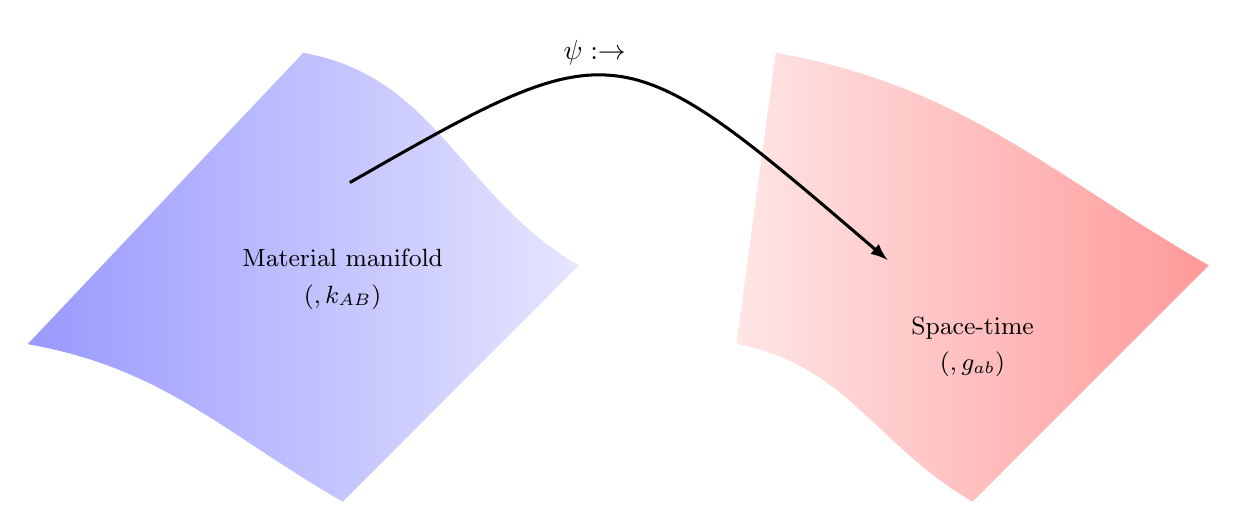
\begin{tikzpicture}
\shade[right color=blue!10,left color=blue!40] 
  (-1,0) to[out=-10,in=150] (3,-2) -- (6,1) to[out=150,in=-10] (2.5,3.7) -- cycle;
  \shade[left color=red!10,right color=red!40] 
  (8,0) to[out=-10,in=150] (11,-2) -- (14,1) to[out=150,in=-10] (8.5,3.7) -- cycle;
  % draw the map
\draw[line,black,line width=1.1pt,shorten >= 3pt,shorten <= 3pt] 
  (3,2) .. controls (6.5,4)   .. (10,1);
 
% we add some labels
\node[font=\color{black}] at (3,1.1) {{\small Material manifold}};
\node[font=\color{black}] at (3,0.6) {{\small $(\matmanif, k_{AB})$}};
\node[font=\color{black}] at (11,0.2) {{\small Space-time}};
\node[font=\color{black}] at (11,-0.25) {{\small$(\stmanif, g_{ab})$}};
\node[font=\color{black}] at (6.2,3.7) {$\psi:\stmanif \rightarrow \matmanif$}; 
\end{tikzpicture}
\caption{Schematic depiction of the  map $\psi$ that associates a point in the material space $\matmanif$ with a point in space-time $\stmanif$. We have also shown which metric is associated with which manifold (and the associated labelling of the indices).}\label{fig:shem_map}
\end{centering}
\end{figure}

\begin{itemize}
\item In Bucher and Spergel, \cite{Bucher:1998mh}, the linearized theory is constructed in detail.
\item See Carter and Quintana \cite{Carter21111972, Carter:1977qf}, Karlovini \cite{Karlovini:2002fc, Karlovini:2003xi, Karlovini:2004gq, Karlovini:2007ut} and \cite{Beig:2002pk, Frauendiener:2007yx, Brito:2009jj, Pourtsidou:2013nha}; \cite{Battye:2005ik}
\cite{Balthazar:2014oza} and \cite{Dubovsky:2011sj}
\item Elasticity and ``hyper -elasticity'' have been further developed in \cite{Carter:1982xm}, \cite{Carter:2006cw}
\item The pull-back idea is very similar to the restoration of non-linear diffeomorphism invariance utilised by massive gravity theories \cite{deRham:2014zqa}.
\item See effective field theory of perfect fluids, \cite{Ballesteros:2012kv}
\item Note that \cite{Karlovini:2002fc} take the tensor $k_{AB}$ to be fixed on the material space.
\item see \cite{Bel:1996pb} \cite{Polak:2007dm}
\item Solids in inflation context \cite{Gruzinov:2004ty, Endlich:2012pz, Bartolo:2014xfa}
\item see \cite{Skovran:2014dka} for exact analytic solutions for perturbed single-component cosmology 
\item \cite{Frauendiener:2007yx}, \cite{Kijowski:1994eq}
\end{itemize}

\subsection{Deformation theory and cosmology}
The current state of affairs in cosmology is that the Universe is accelerating in its expansion, with many avenues being pursued in order to explain this observation. The summary is that the prediction obtained from General Relativity (GR) for how the Universe should look doesn't match up with observations of how the Universe does look (unless, for example, some form of exotic matter is included). One popular way of understanding how to tackle this mis-match is to write the gravitational field equations that actually describes the Universe as
\bea
G_{ab} = 8 \pi G \left(T_{ab} + U_{ab}\right).
\eea
The tensor $U_{ab}$ contains all the deviations or deformations (to begin using the terminology we aim to develop) of the field equations which describe the actual Universe away from the GR (+ standard matter content) predictions. 

The modern cosmology community is busy with developing candidate theories which could provide the components of the tensor $U_{ab}$, and with working out the observation consequences of their given form of the tensor.  We would like to suggest a different approach (or at least, a different philosophy for attacking the problem). Explaining this approach, and showing how it can be used, is the subject of this paper.

In the theory of deformations (in particular, we have in mind   theories of relativistic elasticity) one imagines two states of a material. The first state is a relaxed configuration, and the second is a strained configuration. The deformation which was imparted on the material to take it from being relaxed to being strained isn't necessarily small (if it was small, one would  speak about linear elasticity theory). The theory of deformations prescribes a tool-kit for writing down terms in the field equations which are allowed, given classes or forms of deformation. For example, if the deformation is performed ``on'' some perfect fluid or perfect solid, then it is known that the quantities $U_{ab}$ takes on the form
\bea
\qsuprm{U}{fluid}_{ab} = \rho u_au_b + P\gamma_{ab},\qquad \qsuprm{U}{solid}_{ab} = \rho u_au_b + P_{ab}.
\eea
The energy-momentum tensors written above \textit{become} those for a fluid or solid when some extra theoretical structure is used. Namely, an \textit{equation of state}. For readers who are used to the literature in modern cosmology, this phrase is often used to describe the link between the dark energy pressure $P$ and density $\rho$, via an equation of the form $P(t) = w(t) \rho(t)$. In the context of material models, an equation of state is the Lagrangian density.

When one constructs ``conventional'' models of dark energy or modified gravity, one has a some freedom to choose various types of quantities: these are, e.g., functional forms of the potential, or the kinetic terms which appear in the Lagrangian density. This may seem like an obvious point, but the choice of a restriction on a theory can have implications for (a) its applicability, and (b) its physical naturalness/interpretation. 


\subsection{Fluids and solids}
The distinction between a \textit{fluid} and a \textit{solid} isn't one of the best explained concepts in the literature. Fluids are commonly used as a   description for the content of the Universe in cosmology: but they are only a sub-class of a more general description for ``content''; or, to perhaps use a  more physically transparent terminology: for materials. A more general  description of material is that of a solid; obviously, we won't go so far as to say \textit{the}  general material description. Below we will outline some of the salient pieces to the construction of a material model: full explanations are given in the rest of this paper.

In the descriptions of both solids and fluids  one has a notion of a \textit{material metric} ${k^a}_b$ on a \textit{material space}, whose determinant is related to the particle number density, $n$. A convenient decomposition of this metric is ${k^a}_b = n^{2/3}{\eta^a}_b$. With this decomposition of   ${k^a}_b$, the conformal metric ${\eta^a}_b$ is uni-modular, i.e., it has unit determinant. The action for both a fluid and a solid is of the form 
\bea
\label{eq:intro-solid-action}
S = \int \dd^4x\, \sqrt{-g}\, \ld\left(n, \left[ \gbm{\eta}\right],\left[\gbm{\eta}^2\right]\right).
\eea
Since this is the ``answer'' from which everything else is obtained  it is worth taking a little time to explain the interpretation of various terms. Firstly, $n$ is the number density of particles and is identified with the determinant of the material metric $n = \sqrt{\det k_{AB}}$ on the material manifold (the coordinates $\phi^A$ specify the locations of the particles on the material manifold). The square-braces in (\ref{eq:intro-solid-action}) denote traces of the mixed components of the uni-modular tensor, ${\eta^a}_b = \gamma^{ac}\eta_{cb}$. That is, the action (\ref{eq:intro-solid-action}) is dependant upon the two independent invariants of the tensor
\bea
\eta_{ab} = n^{-2/3}k_{AB}\partial_a\phi^A\partial_b\phi^B.
\eea
It is useful to split up the Lagrangian density   as $\ld = n \epsilon$, where $\epsilon$ is the energy per particle and $n$ retaints its interpretation as the particle number density. In the  cases of   fluids or solids, $\epsilon$ is a function with the following dependencies:
\bea
\qsubrm{\epsilon}{fluid} = \qsubrm{\epsilon}{fluid}(n),\qquad \qsubrm{\epsilon}{solid} = \qsubrm{\epsilon}{solid}(n, {\eta^a}_b).
\eea
This makes the distinction between solids and fluids explicit: it is the dependence of the energy per particle on the uni-modular tensor ${\eta^a}_b$ which makes the description that of a solid rather than a fluid. Later on we will see that the physical consequence of this dependence is that the substance is able to support anisotropic stress (whereas fluids can't): this manifests as \textit{rigidity}. It is worth noting that a fluid is a highly symmetric solid, and a pressureless fluid has $\qsubrm{\epsilon}{fluid}(n) = \overline{\epsilon}_0$, a constant.

In \fref{fig:shem_roadmap} we show how the materials are related.


\tikzstyle{block} = [fill=red!20, draw,rectangle,  text centered, rounded corners, minimum height=2em]
\tikzstyle{block2} = [fill=blue!20,draw,rectangle,  text centered, rounded corners, minimum height=2.5em]
\tikzstyle{block3} = [fill=green!20,draw,rectangle,  text centered, rounded corners, minimum height=2em]
\tikzstyle{block4} = [fill=yellow!5,draw,rectangle,   dotted, text centered, rounded corners, minimum height=2em]

\tikzstyle{line} = [draw,  -latex,   thick]
\tikzstyle{line2} = [draw,  latex-,   thick]
\tikzstyle{cloud} = [ minimum height=2em]

\begin{figure}[!t]
\begin{centering}
\begin{tikzpicture}[node distance = 2cm, auto]
    % Place nodes
    \node [block2] (materialmodels) {{\bf Material models}};
    \node [block3, right of=materialmodels, node distance=5cm] (imperfect) {Viscous};
%    \node [block3, left of=materialmodels, node distance=7cm] (kv) {Visco-elastic solid};
    \node [block3, below right = 1.5cm of materialmodels, node distance=2cm] (solid) {Solid};		
    \node [block3, above left = 1.5cm of materialmodels, node distance=2.5cm] (mixtures) {Mixture};
    \node [block3, above right = 1.5cm of materialmodels, node distance=5cm] (plastic) {Plastic};    
    \node [block3, below left = 1.5cm of materialmodels, node distance=5cm] (fluids) {Fluid};
    \node [block4, below left = 0.5cm of solid, node distance=5cm] (cosmology) {\small Cosmology};
    \node [block4, below right = 0.5cm of solid, node distance=4cm] (nonlinear) {\small Compact objects};
        \node [block, above right = 1.25cm of mixtures, node distance=2cm] (solidscalar) {\small Solid+scalar};
        \node [block, right of=solidscalar, node distance=4cm] (fluidscalar) {\small Fluid+scalar};        
    % Draw edges
    \draw [line] (materialmodels) -- node{\scriptsize perfect}(solid);
    \draw [line] (materialmodels) -- node{\scriptsize example}(fluids);
    \draw [line] (materialmodels) -- node{\scriptsize imperfect}(imperfect);
    \draw [line] (materialmodels) -- node{\scriptsize extra}(mixtures);    
    \draw [line] (materialmodels) -- node{\scriptsize extra}(plastic);        
    \draw [line] (solid) -- node{\scriptsize zero rigidity}(fluids);     
    \draw [line] (solid) -- node{\scriptsize linear}(cosmology);        
    \draw [line] (solid) -- node{\scriptsize non-linear}(nonlinear);           
%    \draw [line] (kv) --  node{\scriptsize Kelvin-Voigt}(cosmology);             
    \draw [line] (mixtures) -- node{\scriptsize hyper-elastic}(solidscalar);             
    \draw [line] (solidscalar) -- node{\scriptsize sub-case}(fluidscalar);         
%    \draw [line] (kv) --  (cosmology);                                
\end{tikzpicture}
\caption{Road-map containing some of the simplest material models. This picture coarsely shows how some of the common classes of materials are related. For example, we see that a fluid is a perfect solid with zero rigidity. We have also shown that the linear theory of solids has been applied to cosmology, and the non-linear theory to compact objects (such as neutron stars).}\label{fig:shem_roadmap}
\end{centering}
\end{figure}
 

{\renewcommand{\arraystretch}{1.4}
\begin{table}%[b] 
%\begin{andptabular}{X[4c]X[4c] }%
\begin{center}
\begin{tabular}{||c |  c ||}
%{Summary  of    commonly used symbols}
\hline
\textbf{Symbol} & \textbf{Meaning} \\
\hline
$\lied{X}$ & Lie derivative operator along the vector $X^{\mu}$\\\hline
$\left(\stmanif, g_{ab}\right)$ & Space-time manifold and metric\\\hline
$\left(\matmanif, k_{ab}\right)$ & Material manifold and metric \\\hline
$u_a$ & Time-like unit-vector; $u^au_a = -1$\\\hline
$\gamma_{ab} = g_{ab} + u_au_b$ & Orthogonal projector; $u^a\gamma_{ab}=0$\\\hline
$n$ & Particle number density; $n^2 = \det k_{AB} $\\\hline
${\eta^a}_b = n^{-2/3}{k^a}_b$ & Uni-modular tensor\\\hline
$\epsilon$ & Equation of state
\\\hline
\end{tabular}\caption{Summary of commonly used symbols}\label{tab:common}
\end{center}
\end{table}
}

Another  concept which is used is that of a \textit{perfect fluid}. This is supposed to be a substance whose energy-momentum tensor can be put into the form
\bea
T_{ab} = \rho u_au_b + P\gamma_{ab},
\eea
in which $\rho$ and $P$ are the  fluid's energy density and pressure respectively, $u^a$ is the velocity of the fluid and $\gamma_{ab} = g_{ab} + u_au_b$ is the orthogonal projection operator. If the energy-momentum tensor for a \textit{fluid} is not of this form (for example, if there is anisotropic stress or heat flux) then the \textit{fluid} is said to be   \textit{imperfect}. We are deliberately being careful about only using the term \textit{fluid}: a solid can be categorised in a similar sense, but a perfect solid manifestly has an anisotropic part to the energy-momentum tensor (this is a distinguishing feature of a solid from a fluid).


In some sense the main result of this review is to obtain an understanding of the theory of a relativistic solid: useful geometric structures on the manifold of particle locations, the action, and energy-momentum tensor. It is rather involved, but is worthwhile since expressions and formulae obtain physical meaning.

\subsection{Conventions}
We use   lower-case latin letters, $a,b,c,\ldots$ to denote space-time indices, and upper-case latin letters, $A, B, C, \ldots$ to denote  indices on the material manifold. The space-time metric is decomposed as
\bea
\label{decomp_g-u-h}
g_{ab} = \gamma_{ab} - u_au_b,
\eea
in which $u_a$ and $\gamma_{ab}$ are the 4-velocity and spatial metric, satisfying
\bea
u^au_a = -1,\qquad u^a \gamma_{ab}=0.
\eea
We use the orthogonally projected derivative
\bea
\label{eq:orth-proj-deri-defn}
\overline{\nabla}_a{A^{b\cdots}}_{c\cdots} = {\gamma^{d}}_a{\gamma^b}_e\cdots {\gamma^f}_c\cdots\nabla_d{A^{c\cdots}}_{f\cdots}
\eea
and the expansion (extrinsic curvature) tensor
\bea
\Theta_{ab} =\overline{\nabla}_{(a}u_{b)}.
\eea
It immediately follows that $\overline{\nabla}_a$ is the connection compatible with $\gamma_{ab}$, since
\bea
\label{eq:sec:overlinenabh=0}
\overline{\nabla}_a \gamma_{cd} =0.
\eea
We will use angular braces to denote the symmetric, trace-free part of a tensor:
\bea
\label{ttls-defin}
A_{\langle ab\rangle} = A_{(ab)} - \tfrac{1}{3}{A^c}_c \gamma_{ab}.
\eea
\subsubsection{First, second, and third fundamental tensors}
Here we briefly review some of Carter's technology \cite{Battye:1995hv, Carter:2000wv, Carter:2011ab} for dealing with branes and imbeddings. 

The idea is that writing ${x^{\mu}}_{,i} = \partial x^{\mu}/\partial \sigma^i$, with $\sigma^i$ the worldsheet coordinates, induces a metric on the world-sheet, $\overline{g}_{ij} = g_{\mu\nu}{x^{\mu}}_{,i}{x^{\nu}}_{,j}$. Instead of working with this quantity (which is written in terms of worldsheet coordinates), it is much more convenient to work with $\overline{g}^{\mu\nu} = \overline{g}^{ij}{x^{\mu}}_{,i}{x^{\nu}}_{,j}$. This invites decomposition of  the space-time metric according to
\bea
\label{eq:sec:decomp_brane_g}
g_{\mu\nu} = \overline{g}_{\mu\nu} + \perp_{\mu\nu}.
\eea
Here $\overline{g}_{\mu\nu}$ is the world-sheet tangential metric: it is the first fundamental form. Also, $\perp_{\mu\nu}$ is orthogonal to the world-sheet. These satisfy
\bea
\overline{g}_{\mu\nu} {\perp^{\mu}}_{\alpha}=0,\qquad \overline{g}_{\beta\nu}\overline{g}^{\alpha\nu} = {\overline{g}^{\alpha}}_{\beta}.
\eea
The  space-time covariant derivative projected into the world-sheet is
\bea
\overline{\nabla}_{\mu} = {\overline{g}^{\alpha}}_{\mu}\nabla_{\alpha}.
\eea
The second fundamental tensor is defined via
\bea
{K_{\mu\nu}}^{\rho} = {\overline{g}^{\sigma}}_{\nu}\overline{\nabla}_{\mu}{\overline{g}^{\rho}}_{\sigma}.
\eea
The first fundamental tensor determines the tangential derivative of the world-sheet metric via
\bea
\label{eq:sec;Kmuab-defn-1}
\overline{\nabla}_{\mu}\overline{g}_{\alpha\beta} = 2 K_{\mu(\alpha\beta)}.
\eea
The second fundamental tensor satisfies
\bea
{\perp^{\mu}}_{\alpha}{K_{\mu\nu}}^{\lambda}=0,\qquad {\overline{g}_{\lambda}}^{\sigma}{K_{\mu\nu}}^{\lambda}=0.
\eea
It is convenient to introduce the extrinsic curvature vector as the trace of the first fundamental tensor,
\bea
K^{\mu} \defn {K^{\alpha}}_{\alpha}{}^{\mu},
\eea
which satisfies
\bea
{\overline{g}^{\mu}}_{\nu}K^{\nu}=0.
\eea

The third fundamental tensor is 
\bea
{\Xi_{\lambda\mu\nu}}^{\rho} \defn {\overline{g}^{\sigma}}_{\mu}{\overline{g}^{\tau}}_{\nu}{\perp^{\rho}}_{\alpha}\overline{\nabla}_{\lambda}{K_{\sigma\tau}}^{\alpha}.
\eea


The more common decomposition of (\ref{eq:sec:decomp_brane_g}) comes in the 3+1 form, via the identifications
\bea
\overline{g}_{\mu\nu} = \gamma_{\mu\nu},\qquad \perp_{\mu\nu} = u_{\mu}u_{\nu}.
\eea
\bea
\nabla_{\mu}\gamma_{\alpha\beta}  =2K_{\mu(\alpha}u_{\beta)}.
\eea
\bea
K_{\mu\alpha\beta} = K_{\mu(\alpha}u_{\beta)}
\eea
It follows that (\ref{eq:sec;Kmuab-defn-1}) evaluates to
\bea
\overline{\nabla}_{\mu}\gamma_{\alpha\beta}.
\eea






\subsection{Perturbed solids}
The majority of this review will be focussed on the general theory of solids: the deformations performed on the solid or medium may be arbitrarily large. Whilst this is very general, it also yields a theory which is complicated to work with. There are a substantial number of physical systems for whom the non-linear theory of elasticity is ``over-kill'': understanding the governing equations that describe small deformations of the solid from its equilibrium configuration is often sufficient. For this reason we shall review the theory of perturbed solids.

Comprehensive reviews, applications, and examples in the relativistic theory have already been presented \cite{Carter:1973zz, Carter:1977qf, Bucher:1998mh, Battye:2005ik, Battye:2007aa, Battye:2013er, Pearson:2014iaa}, as well as the non-relativistic theory being the main subject of a classic book by Landau and Lifshitz \cite{ll_elast}.

The physical picture one should constantly keep in mind is that a continuous medium has ``two states'': relaxed and deformed. The former occurs when there are no forces on the medium, and the latter will induce strains and forces on other surrounding materials and fields (notably the metric). In some sense the ``point'' of a model is to catalogue the possible ways in which a material can influence surrounding media and fields. 

The coordinates of the undeformed medium are represented by $\overline{x}^a$, and those of the deformed medium are by $x^a$. These are related via
\bea
 x^a =  \overline{x}^a+\xi^a(x^b) .
\eea
The crucial piece here is the deformation vector, $\xi^a(x^b)$, which as we explicitly show, is dependent upon the space-time coordinates (different locations can deform by different amounts).

The metric of a space-time which contains a perturbed medium is given by
\bea
\label{metric-perts-elastic}
g_{ab} = \overline{g}_{ab} +h_{ab} + 2 \nabla_{(a}\xi_{b)}.
\eea
The metric of the unperturbed space-time is $\overline{g}_{ab}$, and the metric fluctuations due to ``intrinsic'', or extra-material contents, is given by $h_{ab}$. The presence of the perturbed medium is encapsulated by the term involving the deformation field, 
\bea
\xi^a(x^b) = x^a - \overline{x}^a.
\eea
One may recognise the final term is (\ref{metric-perts-elastic}) as that which arises in standard perturbation theory after one performs the diffeomorphism 
\bea
x^a\rightarrow x^a + \xi^a(x^b).
\eea
Of course, this recognition is accurate. There is an additional concept to appreciate however: interpretation. The $\xi^a$-field describes all the fluctuations of the medium away from its equilibrium configuration. In addition, the deformation field $\xi^a$ is orthogonal,
\bea
u_a\xi^a=0.
\eea

A more elegant, and geometrically intuitive way to write the corrections to the metric is by writing all of the non-background terms in (\ref{metric-perts-elastic}) as
\bea
\lp g_{ab} = \ep g_{ab} + \lied{\xi}g_{ab},
\eea
wherein one can hopefully recognise the usual expression for the Lie derivative of the metric along the vector $\xi^a$,
\bea 
\lied{\xi}g_{ab} = 2\nabla_{(a}\xi_{b)}.
\eea

\subsubsection{Non-relativistic solids}
A non-relativistic solid is one for whom there are no gravitational effects. As examples, one imagines an eraser, rubber band, trampolines: these kinds of materials.

Under a deformation the coordinates of a non-relativistic solid alter according to $x^i \rightarrow x^i + \xi^i(x^j)$. If the line element in the solid before the deformation is $\dd\ell^2 = \delta_{ij} \dd x^i \dd x^j$, then after the deformation the line element has metric  given by
\bea
g_{ij} = \delta_{ij} + 2 \varepsilon_{ij},
\eea
where we defined the strain tensor,
\bea
\label{non-rel-strain-defn}
\varepsilon_{ij}\defn \partial_{(i}\xi_{j)}.
\eea
The components of the strain tensor $\varepsilon_{ij}$ contain all information about the deformation performed on the body. We now require information about the manner in which the body responds to the given deformation. What this actually entails is an understanding of the stress tensor, $\sigma^{ij}$, for a given strain tensor $\varepsilon_{ij}$. If one computes the divergence of the stress tensor one obtains the components of the force, which can be equated to the acceleration of the deformation vectors, to obtain the equation of motion
\bea
\label{nonrela-eom}
F^i = \partial_j\sigma^{ij} = \rho \ddot{\xi}^i.
\eea
In broad-brush-terms there are two possibilities which are useful to consider.
\begin{enumerate}
\item The stress tensor is proportional to the strain tensor:
\bea
\label{e-solid}
\sigma^{ij} = E^{ijkl}\varepsilon_{kl}.
\eea
The components   $E^{ijkl}$ precisely prescribe the strength of certain forces for given deformations (we will have much more to say about this later); they are the components of the elasticity tensor. Materials for whom (\ref{e-solid}) holds are   Hookean elastic solids.
\item The stress tensor is proportional to the rate-of-strain tensor:
\bea
\label{v-solid}
\sigma^{ij} = V^{ijkl}\dot{\varepsilon}_{kl}.
\eea
The components   $V^{ijkl}$ play a similar role to the components of the elasticity tensor for a Hookean solid, except here we are  considering viscous solids and $V^{ijkl}$ are the components of the viscosity tensor.
\end{enumerate}
Of course, the given physical material may require an amalgamation of the two cases, whereby stress is proportional to both strain, and rate-of-strain, in which case
\bea
\label{kv-solid}
\sigma^{ij} = E^{ijkl}\varepsilon_{kl}+ V^{ijkl}\dot{\varepsilon}_{kl}.
\eea
These models describe visco-elastic solids (also known as Kelvin-Voigt solids). Since (\ref{kv-solid}) contains both the elastic (\ref{e-solid}) and viscous (\ref{v-solid}) as sub-cases, we will proceed with the Kelvin-Voigt expression (\ref{kv-solid}). Using (\ref{non-rel-strain-defn}) and (\ref{kv-solid}), the equation of motion (\ref{nonrela-eom}) is
\bea
\label{eom-kv-nonreal}
\rho \ddot{\xi}^i = E^{ijkl}\partial_j\partial_{(k}\xi_{l)} + V^{ijkl}\partial_j\partial_{(k}\dot{\xi}_{l)}. 
\eea

The problem of describing the solid considerably simplifies when one assumes some symmetry of the solid, for example material isotropy. In such cases (other symmetries require more freedom than we are about to introduce), the material tensors only have two independant components each, and decompose completely as
\bse
\label{decomp_iso}
\bea
E^{ijkl} = \left(\beta-\tfrac{2}{3}\mu\right) g^{ij}g^{kl} + 2\mu g^{i(k}g^{l)j},\\
V^{ijkl} = \left(\lambda-\tfrac{2}{3}\nu\right) g^{ij}g^{kl} + 2\nu g^{i(k}g^{l)j}.
\eea
\ese
Using the decompositions (\ref{decomp_iso}), the stress-tensor (\ref{kv-solid}) becomes
\bea
\sigma^{ij} = \left( \beta - \tfrac{2}{3}\mu\right) g^{ij}\partial_k\xi^k + \left( \lambda - \tfrac{2}{3}\nu\right) g^{ij}\partial_k\dot{\xi}^k + 2\mu \partial^{(i}\xi^{j)} + 2 \nu\partial^{(i}\dot{\xi}^{j)},
\eea
and the equation of motion (\ref{eom-kv-nonreal}) becomes
\bea
\label{iso-eom}
\rho \ddot{\xi}^i = \left( \beta + \tfrac{1}{3}\mu\right) \partial^i\partial_k\xi^k + \mu \partial_k\partial^k\xi^i + \left( \lambda + \tfrac{1}{3}\nu\right) \partial^i\partial_k\dot{\xi}^k + \nu \partial_k\partial^k\dot{\xi}^i.
\eea

We shall provide a simple example which highlights the seperate modes of propagation inherent in a material medium. Consider the simple case where the deformation vector has only two components; we can expand $\xi^i$ using two scalars $\phi$ and $\psi$ in an orthonormal basis $(\hat{x}^i, \hat{y}^i)$ via
\bse
\label{iso-eom-ex}
\bea
\xi^i = \phi\hat{x}^i + \psi\hat{y}^i.
\eea
Now suppose that these scalars depend on time, and only one of the two available spatial directions; that is, we set
\bea
\partial_i\phi = \phi'\hat{x}_i,\qquad \partial_i\psi = \psi'\hat{x}_i.
\eea
\ese
Putting the decomposition of the deformation vector (\ref{iso-eom-ex}) into the equation of motion (\ref{iso-eom}) yields an equation with two independant projections (one along $\hat{x}^i$, and one along $\hat{y}^i$); these projections leads to the requirement that the following two equations are satisfied:
\bea
\ddot{\phi} - \frac{\lambda + \frac{4}{3}\nu}{\rho}\dot{\phi}'' = \frac{\beta+\frac{4}{3}\mu}{\rho}\phi'',\qquad
\ddot{\psi} - \frac{\nu}{\rho}\dot{\psi}'' = \frac{\mu}{\rho}\psi''.
\eea
In the purely elastic case (i.e., where all components of the viscosity tensor vanish), it is with relative ease that one realises a plane wave ansatz $\phi \sim e^{\ci\left( \omega t + kx \right)}$ solves the equations of motion, and that $\phi$ and $\psi$ travel with different speeds: these are the  longitudinal and transverse sound speeds
\bea
\qsubrm{c}{L}^2 = \frac{\beta + \frac{4}{3}\mu}{\rho},\qquad \qsubrm{c}{T}^2 = \frac{\mu}{\rho}.
\eea
\subsubsection{Relativistic solids}



\cleardoublepage
\section{Describing non-linear materials}
In this section we will take some time to build a description of a medium. We will introduce the notion of a material manifold, and geometric structures on the material manifold: coordinates, metric, connection, and volume form. There will be an important step where we relate structures in the material manifold to structures in space-time. We will want to obtain fields and energies in space-time due to structures in the material manifold. There will be some instances where we ``mix'' material space and space-time indices; this is   unavoidable in the course of exposing some interesting part of the formalism. That said, all final results (equations of motion etc) will be expressed solely in terms of space-time indicies.
\subsection{The material manifold,  particle number density, and map}
\label{sec:mpnd}
It is important to understand the minimal assumed geometric structure in building a model. We  assume that there is a 3D   manifold $\matmanif$ which is endowed with a particle density form $n_{ABC} = n_{[ABC]}$. This is the material manifold. There will be an associated metric on the material manifold, which we call $k_{AB}$ and will discuss further later on. 

The points of $\matmanif$ are  particles of the medium, and they do not move: the dynamics in space-time comes from the maps from the material manifold to space-time, not the motion of the particles in material space.  We shall let  $\stmanif'$ be the submanifold of the full space-time manifold $\stmanif$  which is the subset of the spacetime that the material passes through. Then invoke a map $\psi$ which takes a location in space-time and points at a location in the material manifold;
\bea
\psi : \stmanif'\longrightarrow \matmanif.
\eea
For all points p in $\matmanif' = \psi(\stmanif')$, the inverse map at that point, $\psi^{-1}({\rm p})$, is a single time-like curve in $\stmanif'$: these are the flow-lines of the particles. 

Let $\phi^A$ be   coordinates in material space. Then their gradients with respect to the space-time coordinates $x^a$ can be computed
\bea
\label{eq:sec:config_gradient}
{\psi^A}_a = \pd{\phi^A}{x^a}.
\eea
The ${\psi^A}_a$ are   the components of the configuration gradient. The time-like projection of these must vanish
\bea
\label{eq:sec:ortho-condition}
u^a{\psi^A}_a =0.
\eea
This is equivalent to setting the Lie derivative of the $\phi^A$ in the time-like direction to zero:
\bea
\lied{u}\phi^A=0,
\eea
which has a more direct physical interpretation of saying that the material coordinates are static with respect to coordinate time. In Section \ref{sec:hyperelasticity} we shall explain what happens when this condition is relaxed: the upshot is that one ends up describing ``scalar field theories'', rather than ``solid theories''.  In that section we also explore the technology required when the material manifolds dimension isn't just three, and where the material lives on some brane in a higher dimensional bulk.

One can conceive of scalars, vectors, forms, and tensors on the material manifold: the material metric and particle density form are examples, as are a few other tensors we introduce later on. Collectively, we call such quantities ``material tensors'', and they have components whose indices are denoted with captial latin letters. We relate tensors in the material and space-time manifolds using the technology of pull-backs and push-forwards:
\begin{itemize}
\item $\psi^{\star}$ is the pull-back of a covariant tensor from $\matmanif'$ to $\stmanif'$ and is denoted to act on a material tensor as
\bea
N_{ab\cdots z} = \psi^{\star} N_{AB\cdots Z}.
\eea
In ``coordinates'' notation the pull-back is
\bea
\label{eq:sec:coord-pull-bacj}
N_{ab\cdots z} = {\psi^A}_a{\psi^B}_b \cdots {\psi^Z}_z N_{AB\cdots Z},
\eea
where ${\psi^A}_a$ are the components of the configuration gradient (\ref{eq:sec:config_gradient}). 
\item $\psi_{\star}$ denotes the push-forward of a contravariant tensor from $\stmanif'$ to $\matmanif'$, and is denoted to act on a space-time tensor as
\bea
M^{AB\cdots Z} = \psi_{\star}M^{ab\cdots z},
\eea
and in coordinates it reads
\bea
\label{eq:sec:pusg-frwad-explanation}
M^{AB\cdots Z}= {\psi^A}_a{\psi^B}_b \cdots {\psi^Z}_z M^{ab\cdots z}.
\eea
\end{itemize}

The most important corollary of (\ref{eq:sec:ortho-condition}) is that any tensor on space-time which was constructed as the pull-back of a tensor on the material space will   automatically be orthogonal. That is, for the schematic example (\ref{eq:sec:coord-pull-bacj}),
\bea
u^aN_{ab\cdots z}  = u^bN_{ab\cdots z}  =\cdots = u^zN_{ab\cdots z}=  0.
\eea

The integral of the particle number density form $n_{ABC}$ over some volume in the material manifold $\matmanif$ is the number of particles in that volume (by definition). The pull-back of the particle volume-form to   space-time   is
\bea
n_{abc} = \psi^\star n_{ABC}.
\eea
Note that the property (\ref{eq:sec:ortho-condition}) makes $n_{abc}$ an orthogonal space-time field.
Using   the space-time volume form $\epsilon_{abcd}$ the particle current $n^a$ is
\bea
\label{eq:sec:na-defin}
n^a = \frac{1}{3!}\epsilon^{abcd}n_{bcd},
\eea
and is manifestly conserved,
\bea
\label{eq:sec:conse-n}
\nabla_an^a = 0.
\eea
This conservation follows since $n_{abc}$ is a closed 3-form due to $n_{ABC}$ being a closed 3-form on material space (an $n$-form in $n$-dimensional space is closed). What this also means is that to break (\ref{eq:sec:conse-n}) and have $\nabla_an^a\neq 0$ one requires $n^a$ not to be related to the volume form on material space: i.e., there is no volume form on material space. Note that the particle current $n^a$ is the dual of the volume form $n_{abc}$.

It follows by orthogonality of $n_{abc}$ that the particle current (\ref{eq:sec:na-defin}) is time-like
\bea
\label{eq:sec:n-u-n}
n^a = nu^a,
\eea
where the particle number density $n$ is given by
\bea
n = \sqrt{-n^an_a}.
\eea
We have
\bea
\label{eq:sec:n-u-n-1}
\epsilon_{abc} = \epsilon_{abcd}u^d ,\qquad n_{abc} = n \epsilon_{abc}.
\eea
A useful invariant is
\bea
n^2 = \frac{1}{3!}n^{abc}n_{abc}.
\eea
Note that from the conservation equation for $n^a$, (\ref{eq:sec:conse-n}), and (\ref{eq:sec:n-u-n}), one obtains an evolution equation for the particle number density,
\bea
\label{ev_n}
\dot{n} = - n\Theta,
\eea
where $\Theta = {\Theta^a}_a$ is the trace of the extrinsic curvature tensor.
 
Another way  of writing down (\ref{eq:sec:na-defin}) is found after combining (\ref{eq:sec:n-u-n}) and (\ref{eq:sec:n-u-n-1}) to give
\bea
\label{eq:sec:nabc_dual_na}
n_{abc} = \epsilon_{abcd}n^d.
\eea
The expression (\ref{eq:sec:nabc_dual_na}) directly shows that the 3-form $n_{abc}$ is the dual to $n^a$, and will highlight the connection to Kalb-Ramond fields. A Kalb-Ramond field is a 2-index object that transforms as a 2-form; its components satisfy
\bea
B_{ab} = B_{[ab]}.
\eea
The  3-form field strength $F_{abc}$ corresponding  to $B_{ab}$ is an exact form constructed by taking the ``derivative''
\bse
\bea
F = \dd B,
\eea
which works out in this case as
\bea
F_{abc} = 3\nabla_{[a}B_{bc]}.
\eea
\ese
Since $F_{abc}$ is an exact form, it is therefore a closed form\footnote{A \textit{closed} form $C$, say, is a form for whom $\dd C=0$. Let $A$ be a $p$-form, then $F = \dd A$ is an \textit{exact} $(p+1)$-form. Since $\dd^2=0$, it follows that $\dd F=0$; in words this statement is: \textit{an exact form is a closed form}.}: the expression of  automatic closure is given by 
\bea
\label{F-closed}
\nabla_{[a}F_{bcd]}=0.
\eea
Related to the 3-form field strength $F_{abc}$  is  its dual $\widetilde{F}^a$, which is constructed via
\bea
F_{abc} = \epsilon_{abcd}\widetilde{F}^d.
\eea
By virtue of the automatic closure (\ref{F-closed}) it follows that $\widetilde{F}^a$ is conserved,
\bea
\nabla_a\widetilde{F}^a=0.
\eea
It should therefore be clear that the particle number density current $n^a$, which is the dual of the number density form $n_{abc}$, is the field strength tensor of some field of Kalb-Ramond type. \comment{It is worth finding \cite{Carter:1994rv}}

\subsection{Material metric}
\label{sec:mat-metric}
We invoke the existence of a metric $k_{AB}$ on the material manifold $\matmanif$ whose volume form is the particle density form $n_{ABC}$ introduced in Section \ref{sec:mpnd}. This metric will enable us to introduce a Levi-Civita connection in the material manifold, which can be pulled-back to space-time to aid the evaluation of derivatives of material tensors. Before we explain this fairly complicated construction we shall elucidate some other useful structures on the material manifold.


Indices on material tensors can be contracted with the indices of other material tensors. Equivalently, indices on space-time tensors    can also be contracted with those of other space-time tensors (a space-time scalar can be formed if contraction leaves no spare indices). Importantly, space-time tensors can be the pulled-back version of a material tensor, as in the discussion in the previous section. As an example, consider an arbitrary material tensor $A_{ABC\cdots}$ which is ``pulled-back'' to give a space-time tensor $A_{abc\cdots}$ according to the usual prescription $A_{abc\cdots} = \psi^{\star}A_{ABC\cdots}$. Then, after contracting some indices with the space-time metric,
\bea
B_{c\cdots} =  g^{ab}A_{abc \cdots} = g^{ab}\psi^{\star} A_{ABC\cdots}
\eea
is a legitimate space-time tensor.  One can also     contract indices of material tensors on the material manifold $\matmanif$, with the push-forward of space-time tensors. As an example, consider the push-forward of the inverse space-time metric tensor 
\bse
\bea
\label{eq:sec:push-fwd-metric}
g^{AB} = \psi_{\star} g^{ab} 
\eea
being contracted with an arbitrary material tensor,
\bea
g^{AB} C_{ABC\cdots} = \psi_{\star} g^{ab}C_{ABC\cdots}.
\eea
 From the orthogonality of the material mappings it follows that 
\bea
g^{AB} = \psi_{\star}\gamma^{ab},
\eea
\ese 
where we remind that $\gamma^{ab}$ is the orthogonal part of the space-time metric as defined in (\ref{decomp_g-u-h}). 

Note that $g^{AB}$ is the push-forward of the space-time metric to the material manifold, and does not necessarily coincide with the material metric $k_{AB}$. Infact, quantifying its non-coincidence is extremely important in quantifying the state of a  material. With this in mind, we define a material tensor  $\eta_{AB}$, which depends on the number density $n$, such that the push-forward of the space-time metric $g^{AB}$ is exactly the inverse of $\eta_{AB}$ when the material is in its unsheared state. That is,  $g^{AC}\eta_{CB} = {\delta^A}_B$ (the Kronecker-delta) when the energy is at its minimum $\epsilon = \check{\epsilon}(n)$. What this means is that $g^{AB} = \eta^{-1AB}$ in what is henceforth defined as the \textit{unsheared state}. Consequently, the deviation of the actual value of $g^{AB}$ from $\eta^{-1AB}$, which we write as
\bea
\label{material-space-s}
s^{AB} =\tfrac{1}{2}\left( g^{AB} - \eta^{-1AB}\right),
\eea
quantifies the shear of the system.  

Writing the volume form of $\eta_{AB}$ as $\epsilon_{ABC}$ it follows that
\bea
n_{ABC} = n \epsilon_{ABC}.
\eea
Note that   $\epsilon_{abc} = \psi^{\star}\epsilon_{ABC}$.
The particle density form $n_{ABC}$ is a fixed material space tensor, and is independent of $n$. 

It is now useful and helps physical insight, to define the material tensor $k_{AB}$ as the metric on the material manifold $\matmanif$. $k_{AB}$ is conformal to $\eta_{AB}$, and has the particle density form $n_{ABC}$  as its volume form. Therefore
\bea
\label{eq:k-eta-n-defn}
k_{AB} = n^{2/3}\eta_{AB}.
\eea
This tells us that the (square-root of the) determinant of $k_{AB}$ is the particle number density, $n$:
\bea
n = \sqrt{\det k_{AB}}.
\eea
See \fref{fig:obj_links} for a cartoon of the relationship between the material metric $k_{AB}$ and particle form $n_{ABC}$.

 
\tikzstyle{block} = [fill=red!20, draw,rectangle,  text centered, rounded corners, minimum height=2em]
\tikzstyle{block2} = [fill=blue!20,draw,rectangle,  text centered, rounded corners, minimum height=2.5em]
\tikzstyle{block3} = [fill=green!20,draw,rectangle,  text centered, rounded corners, minimum height=2em]
\tikzstyle{block4} = [fill=yellow!5,draw,rectangle,   dotted, text centered, rounded corners, minimum height=2em]

\tikzstyle{line} = [draw,  -latex,   thick]
\tikzstyle{line1} = [draw,  dotted, thick]
\tikzstyle{line2} = [draw,  latex-,   thick]
\tikzstyle{cloud} = [ minimum height=2em]

\begin{figure}[!t]
\begin{centering}
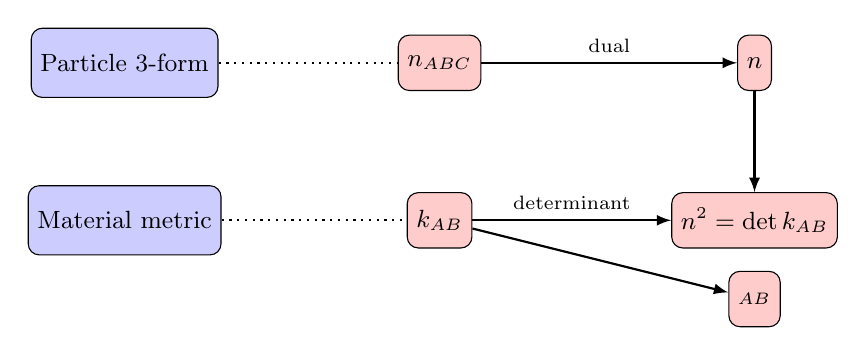
\begin{tikzpicture}[node distance = 2cm, auto]
    % Place nodes
    \node [block2] (form) {{\small Particle 3-form}};
    \node [block, right of=form, node distance=4cm] (form_1) {\small $n_{ABC}$};   
    \node [block, right of=form_1, node distance=4cm] (form_2) {\small $n$};        
    \node [block2, below of=form] (metric) {{\small Material metric}};        
    \node [block, right of=metric, node distance=4cm] (metric_1) {\small $k_{AB}$};     
    \draw [line1] (metric) -- (metric_1);
    \node [block, right of=metric_1, node distance=4cm] (metric_2) {\small $n^2 = \det k_{AB}$};        
    \node [block, below of=metric_2, node distance=1cm] (metric_3) {\small $\unimod_{AB}$};            
    % Draw edges
    \draw [line1] (form) -- (form_1);
    \draw [line] (form_1) -- node{\scriptsize dual}(form_2);
        \draw [line] (metric_1) -- node{\scriptsize determinant}(metric_2);
    \draw [line] (form_2) -- (metric_2);    
       \draw [line] (metric_1) -- (metric_3);        
\end{tikzpicture}
\caption{Explanation of the link between geometrical objects in  the particle 3-form and material-metric formulations of elasticity theory. In the ``particle 3-form'' formulation, the only peice of information about the geometrical structure of the material manifold that is actually used is $n$, the dual of the particle 3-form. In the ``material metric'' formulation, one posits a metric on the material manifold which has more pieces of information which are used: its determinant, $n$, and quantites $\eta_{AB}$ which keep track of the shear-like parts of $k_{AB}$. The point is that the material metric construction keeps track of more information about the material manifold than the particle 3-form construction. In this way the former is more general than the latter.}\label{fig:obj_links}
\end{centering}
\end{figure}
  

The pull-back of $k_{AB}$ gives a space-time tensor,
\bea
\label{eq:sec:k_abdefn}
k_{ab} = \psi^{\star}k_{AB},
\eea
and will play an important role in what follows.  Specifically, using (\ref{eq:sec:coord-pull-bacj}) the pull-back (\ref{eq:sec:k_abdefn}) reads
\bea
\label{pullbackk}
k_{ab} =  {\psi^A}_a{\psi^B}_b k_{AB}.
\eea
An application of   (\ref{eq:sec:ortho-condition}) is that since $k_{ab}$ is a  space-time field, it is orthogonal
\bea
u^ak_{ab}=0.
\eea
We will frequently use the mixed version of the tensor, wherein indices are raised with the space-time metric,
\bea
\label{eq:sec:defn-kmixed-0}
{k^a}_b = g^{ac}k_{bc},
\eea
which is also orthogonal,
\bea
\label{eq:sec:orthn-k}
u^a{k^b}_a=0.
\eea
As a consequence of (\ref{eq:sec:orthn-k}), (\ref{eq:sec:defn-kmixed-0}) can be re-expressed as
\bea
\label{eq:sec:defn-kmixed}
{k^a}_b = \gamma^{ac}k_{bc}.
\eea
From (\ref{eq:sec:defn-kmixed}) it follows that
\bea
\pd{{k^a}_b}{g^{cd}} = {\delta^a}_{(c}k_{d)b}.
\eea
Similarly,  the pull-back of $\eta_{AB}$ gives an orthogonal space-time tensor
\bea
\label{eq:sec:eta_abdefn}
\eta_{ab} = \psi^{\star}\eta_{AB},
\eea
and we also use the mixed version of the tensor,
\bea
\label{eq:sec:etamixed-defn}
{\eta^a}_b = \gamma^{ac}\eta_{cb}.
\eea
From the pull-back of the relationship (\ref{eq:k-eta-n-defn}) we obtain 
\bea
\label{eq:sec:k-eta-n-pb}
{k^a}_b = n^{2/3}{\eta^a}_b.
\eea

Since we have set everything up so that $n^2$ is the determinant of $k_{ab}$, it follows from (\ref{eq:sec:k-eta-n-pb}) that ${\eta^a}_b$ is a uni-modular tensor:
\bea
\det({\eta^a}_b)=1.
\eea 
This property will be useful later on.

We now elucidate some consequences of the $n$-dependence of $k_{AB}$.
In what follows it will be convenient to denote differentiation with respect to $n$ with a prime. Using (\ref{eq:k-eta-n-defn}) to compute $k_{AB}'$ yields
\bea
\label{eq:sec:tobetraced01}
n\eta'_{AB} = - \tfrac{2}{3}\eta_{AB} + \tau_{AB},
\eea
in which
\bea
\label{defn_tauAB}
\tau_{AB} \defn n^{1/3}k'_{AB}.
\eea
Since $n'_{ABC}=0$ (by definition) it follows that $(\det k_{AB})'=0$, and therefore $k^{-1AB}k_{AB}'=0$, and hence
\bea
\eta^{-1AB}\tau_{AB}=0.
\eea
Thus, we see that $\tau_{AB}$ is   traceless; it is called the \textit{compressional distortion tensor}, and measures   deformations of the medium that \textit{aren't} due to conformal rescalings of the material metric upon varying the particle density.
Hence, computing the trace of (\ref{eq:sec:tobetraced01}) with respect to $\eta^{-1AB}$ yields
\bea
n\eta^{-1AB}\eta'_{AB}=-2.
\eea
Note that from (\ref{defn_tauAB}) it follows trivially, but more usefully, $k'_{AB} = n^{-1/3}\tau_{AB}$, and so if the material varies only  conformally (i.e. is uniformly compressed) $k_{AB}$ is independent of $n$ since $\tau_{AB}=0$ for these types of deformations.


The push-forward of (\ref{eq:sec:tobetraced01}) reads
\bea
n\eta_{ab}' = - \tfrac{2}{3}\eta_{ab} + \tau_{ab}.
\eea
And so, in the case where $\eta_{ab} = \eta_{ab}(n)$, it is simple to see that
\bea
[{\eta}_{ab}]^{\cdot} = \eta'_{ab}[n]^{\cdot},
\eea
where $[X]^{\cdot}$ denotes the material derivative of $X$. After using (\ref{ev_n}) to replace $[n]^{\cdot}=\dot{n}$ we obtain the evolution equation:
\bea
[{\eta}_{ab}]^{\cdot} =  \left( \tfrac{2}{3}\eta_{ab} - \tau_{ab}\right)\Theta.
\eea



\subsection{Material covariant derivative}
It is convenient at this point to introduce the covariant derivative on the material manifold which is compatible with the material metric. Let $\overline{\widetilde{\nabla}}_A$ be the Levi-Civita connection for $k_{AB}$; i.e.,
\bea
\overline{\widetilde{\nabla}}_C k_{AB}=0.
\eea
There is a reason for our including two different ``accents'' above the del-symbol.
The pushed-forward version of $\overline{\widetilde{\nabla}}_A$, denoted as $\overline{\widetilde{\nabla}}_a$, is allowed to act on space-time tensors; note that it will be orthogonal, and so is taken to be the orthogonal projection of some space-time derivative $\widetilde{\nabla}_a$ according to
\bea
\overline{\widetilde{\nabla}}_a{A^{b\cdots}}_{c\cdots} = {\gamma^{d}}_a{\gamma^b}_e\cdots {\gamma^f}_c\cdots\widetilde{\nabla}_d{A^{c\cdots}}_{f\cdots}.
\eea
For any space-time vector $Y^a$ the difference between any two connections can be written as
\bea
\label{eq:sec:intro-d-defn-flsdhfkdgh}
\left(\overline{\widetilde{\nabla}}_a- \overline{\nabla}_a\right)Y^c = {\mathfrak{D}^c}_{ab}Y^b
\eea
in which  $ {\mathfrak{D}^c}_{ab}$ is the (symmetric) relativistic   difference tensor \footnote{The conditions required for this definition to hold are} defined as
\bea
\label{eq:sec:defn-D-ela-diff-tensor}
{\mathfrak{D}^c}_{ab} = \tfrac{1}{2}k^{-1cd}\left( \overline{\nabla}_ak_{bd} + \overline{\nabla}_bk_{ad} - \overline{\nabla}_dk_{ab}\right),
\eea
where $k^{-1cd}$ is defined via
\bea
k^{-1cd} k_{ca} = {\gamma^d}_a, 
\eea
and is orthogonal $ k^{-1cd}u_c = 0$. Due to the applications in mind, we actually call ${\mathfrak{D}^c}_{ab}$ the relativistic elasticity difference tensor.

Using this construction, one finds that $\overline{\widetilde{\nabla}}_a$ is the connection which is compatible with $k_{ab}$,
\bea
\label{bartildenabk=0}
\overline{\widetilde{\nabla}}_ak_{cd} =0.
\eea
As an example of using this technology, suppose that ${B^{a\cdots}}_{b \cdots}$ is a tensor function of $g^{ab}$ and $k_{ab}$. Then taking its derivative with $\overline{\widetilde{\nabla}}_a$  yields
\bea
\overline{\widetilde{\nabla}}_a{B^{b\cdots}}_{c \cdots} = \pd{{B^{b\cdots}}_{c \cdots}}{g^{ef}} \overline{\widetilde{\nabla}}_a{g^{ef}} + \pd{{B^{b\cdots}}_{c \cdots}}{k_{ef}}\overline{\widetilde{\nabla}}_a{k_{ef}}= \pd{{B^{b\cdots}}_{c \cdots}}{g^{ef}} \overline{\widetilde{\nabla}}_a{g^{ef}} ,
\eea
where the second equality holds via (\ref{bartildenabk=0}). We can go one step further and realise that
\bea
\overline{\widetilde{\nabla}}_a{B^{b\cdots}}_{c \cdots} = \pd{{B^{b\cdots}}_{c \cdots}}{g^{ef}} \left(\overline{\widetilde{\nabla}}_a{g^{ef}} -\overline{ {\nabla}}_a{g^{ef}} \right) = 2  \pd{{B^{b\cdots}}_{c \cdots}}{g^{ef}} {\mathfrak{D}^{ef}}_a.
\eea
The second term in braces, $\overline{ {\nabla}}_a{g^{ef}}$, vanishes by (\ref{eq:sec:overlinenabh=0}), and the final equality holds by (\ref{eq:sec:intro-d-defn-flsdhfkdgh}). Finally, since
\bea
\overline{{\nabla}}_a{B^{b\cdots}}_{c \cdots} = \overline{\widetilde{\nabla}}_a{B^{b\cdots}}_{c \cdots}  - \left(  \overline{\widetilde{\nabla}}_a-\overline{{\nabla}}_a\right){B^{b\cdots}}_{c \cdots},
\eea
 then it follows by repeated application of (\ref{eq:sec:intro-d-defn-flsdhfkdgh}) on the last term, that orthogonally projected derivative is
\bea
\label{overlineDB}
\overline{{\nabla}}_a{B^{b\cdots}}_{c \cdots} &=& 2 \pd{{B^{b\cdots}}_{c \cdots} }{g^{de}}{\mathfrak{D}^{de}}_a  - {B^{d\cdots}}_{c\cdots} {\mathfrak{D}^{b}}_{ad} - \cdots + {B^{b\cdots}}_{d\cdots} {\mathfrak{D}^{d}}_{ac} + \cdots. 
\eea


\subsection{Constructing the set of scalar invariants}
\label{sec-setscalinvs}
We will formally introduce it later, but we are interested in constructing  the equation of state $\rho$ which will be a scalar function of the state of the system which is integrated to give the action. There are a few different sets of scalar invariants one could use: formally they are identical, but different choices will enhance, or hide,  insight  into the  physical behavior. And so, we are interested in finding  the complete list of scalar invariants which will specify the state of the system.  The invariants are constructed from the pull-back of the material metric, ${k^a}_b$.

As a candidate set of invariants, note that \textit{the} three independent scalar invariants of the mixed components of the pulled-back material metric ${k^a}_b$ are
\bea
I_1 = [\rbm{k}],\qquad I_2 = [\rbm{k}^2],\qquad I_3 = [\rbm{k}^3],
\eea
in which we   denoted   traces with square braces,
\bea
I_n = \Tr(\rbm{k}^n) = [\rbm{k}^n] = {k^a}_b{k^b}_c\cdots{k^f}_a ,
\eea
with ${k^a}_b$ defined from $k_{ab}$ via (\ref{eq:sec:defn-kmixed}). This is a complete list of independent invariants (any other invariants can be computed from these) due to the orthogonality of ${k^a}_b$ (\ref{eq:sec:orthn-k}).
Since $n_{ABC}$ is the volume form of $k_{AB}$, the particle number density $n$ is also a scalar invariant of ${k^a}_b$; by the Cayley-Hamilton theorem, the determinant is related to the other invariants via
\bea
n^2 = \det({k^a}_b) = \tfrac{1}{3!}\left([\rbm{k}]^3 - 3[\rbm{k}][\rbm{k}^2] + 2 [\rbm{k}^3]\right).
\eea

We  could use $\{I_1,I_2,I_3\}$ as the list of invariants which could be the arguments of the equation of state, but we shall instead choose $n$ and  the independent scalar invariants of the uni-modular tensor ${\eta^a}_b$, defined in (\ref{eq:sec:etamixed-defn}) since this will help the comparison between solid and fluid descriptions. The important consequence of   uni-modularity is that     ${\eta^a}_b$   only has two independent invariants (rather than 3 which could be expected from a symmetric rank-2 tensor in 3D).  The invariants are linked via the Cayley-Hamilton theorem as
\bea
\label{eq:sec:eta-link-invariants}
3! = [\gbm{\eta}]^3 - 3 [\gbm{\eta}][\gbm{\eta}^2] + 2 [\gbm{\eta}^3].
\eea
Notice that (\ref{eq:sec:eta-link-invariants}) can be rewritten as
\bea
2\left([\gbm{\eta}^3] -3   \right)= 3[\gbm{\eta}]\left( [\gbm{\eta}^2] - \tfrac{1}{3}[\gbm{\eta}]^2\right).
\eea

To summarise, we have  shown that there are two  equivalent   ways to write the most general equation of state for a solid: both have a maximum of three arguments. They are
\bse
\bea
\rho = \rho\left([\rbm{k}],\left[\rbm{k}^2\right],\left[\rbm{k}^3\right]\right)
\eea 
and
\bea
\rho = \rho\left(n, [\gbm{\eta}],\left[\gbm{\eta}^2\right]\right).
\eea
\ese
We remind that ${k^a}_b$ is the pull-back of a tensor whose volume form is $n_{ABC}$ and (squared) determinant is the particle number density, $n$. Secondly, ${\eta^a}_b$ is a uni-modular tensor whose inverse $\eta^{-1AB}$ co-incides with the push-forward of the space-time metric when the material is in the unsheared state. The latter formulation is somewhat favorable, since it becomes easy to connect to a scenario in which the solid ``becomes'' like a fluid, since $\rho$ becomes independent of $[\gbm{\eta}^n]$.
 
 
Before we continue it is worth noting some useful ways to compute derivatives of functions which depend on quantities which regularly appear in the construction, most notably functions which depend on $n$ or ${\eta^a}_b$.
First of all, the derivative of the number density $n$ with respect to the space-time metric is given by
\bea
\label{eq:sec:dndg}
\pd{n}{g^{ab}} = \half n \gamma_{ab}.
\eea
When $Y = Y({k^a}_b)$ is any quantity that depends only on the ${k^a}_b$,  then its derivative with respect to the space-time metric is
\bea
\label{eq:pd-Y-g-k}
\pd{Y}{g^{ab}} = k_{c(a}\pd{Y}{{k^{b)}}_c}.
\eea
For any quantity $Z = Z(n,{\eta^a}_b)$, and using (\ref{eq:sec:k-eta-n-pb}) as a decomposition of the degrees of freedom in ${k^a}_b$, we obtain
\bea
\label{eq:sec:Zneta}
\pd{Z}{g^{ab}} = \half n\gamma_{ab}\pd{Z}{n} + \eta_{c\langle a}\pd{Z}{{\eta^{b\rangle}}_c},
\eea
where the angular brackets denote the symmetric trace-free part of the tensor, as defined in (\ref{ttls-defin}). For each quantity $n$, $Y$, and $Z$ as defined here,
\bea
u^a\pd{n}{g^{ab}} =0,\qquad u^a\pd{Y}{g^{ab}}=0,\qquad u^a\pd{Z}{g^{ab}}=0.
\eea
 



\subsection{Deformations about a relaxed state}
It is   important to understand how to deal with a deformed medium. Before we give some explicit expressions for  deformations of the solid, we shall illustrate the philosophy via ``non-linear sigma models'' from field theory.
\subsubsection{Example from non-linear sigma models}
One of the important ideas in continuous mechanics is that of the assumed existence of a relaxed state: this is supposed to be some configuration that minimizes some measure of ``energy''. This concept is absolutely vital in the study of solitons. As the simplest example, consider the Lagrangian density for a real scalar field $\phi$ living in a Higgs potential,
\bea
\label{eq:lag-dw-1}
\ld = - \half \partial_{a}\phi\partial^{a}\phi - \frac{\lambda}{4}\left( \phi^2 - \eta^2\right)^2.
\eea
The relaxed configuration of this scalar is when $\phi = \pm \eta$ (commonly known as the vacuum manifold). It is simple to find the Lagrangian density for fluctuations about the relaxed state; substituting $\phi = \eta + \delta\phi$ into (\ref{eq:lag-dw-1}) and expanding to quadratic order in $\delta\phi$ yields
\bea
\ld = - \half \partial_{a}\delta\phi\partial^{a}\delta\phi - \half \lambda \eta^2(\delta\phi)^2.
\eea
The Lagrangian that results is that for a massive scalar field. This example is depressingly simple since there isn't a non-trivial Lagrangian that describes the field \textit{in} the relaxed state. For that we shall move to a more complicated example and think about a multi-scalar field model whose Lagrangian density is
\bea
\label{eq:sec:lag-full}
\ld =- \half \mathfrak{k}_{IJ}\partial_{a}\Phi^I\partial^{a}\Phi^J- V(\Phi^I).
\eea
There are supposed to be $n$ fields here, and so $I = 1, \ldots, n$, and the set of symmetric quantities $ \mathfrak{k}_{IJ}$ are supposed to play the role of a  metric in field space.
Before we continue we want to make it plainly clear that this isn't the most general Lagrangian density that can be constructed out of single derivatives. 

 Suppose that the energy gets minimized when the fields $\Phi^I$ are consigned to live on a sub-manifold, $\mathcal{V}$ say, of dimension $q \leq n$. The ``vacuum manifold'' $\mathcal{V}$ can be coordinatized by $q$ scalars $\phi^A$, say, with $A = 1, \ldots, q$. Hence, the original set of fields $\Phi^I$ are some function of the fields $\phi^A$,
\bea
\label{eq:sec:relaxed-config}
\Phi^I = \Phi^I(\phi^A),
\eea
when the configuration is in its relaxed state. From (\ref{eq:sec:relaxed-config}) it is clear that
\bea
\label{eq:sec:parti-phiI-phiA}
\partial_{a}\Phi^I = \pd{\Phi^I}{\phi^A}\partial_{a}\phi^A.
\eea
Putting (\ref{eq:sec:parti-phiI-phiA}) into (\ref{eq:sec:lag-full}) gives 
\bea
\label{eq:lag-eff-phiA}
\ld = - \half \mathfrak{g}_{AB}(\phi)\partial_{a}\phi^A\partial^{a}\phi^B,
\eea
in which we defined
\bea
\label{eq:sec:GAB-met}
\mathfrak{g}_{AB}(\phi) \defn  \mathfrak{k}_{IJ}\pd{\Phi^I}{\phi^A}\pd{\Phi^J}{\phi^B},
\eea
which is interpreted as the metric on the field submanifold $\mathcal{V}$.   The field equations for the $\phi^A$ derived from (\ref{eq:lag-eff-phiA})   are given by
\bea
g^{ ab}\nabla_{a}\nabla_{b}\phi^A + \cs{A}{B}{C}\nabla_{a}\phi^B\nabla^{a}\phi^C=0,
\eea
where
\bea
\label{eq:cs-sigmamodel}
\cs{A}{B}{C} = \tfrac{1}{2} \mathfrak{g}^{AD}\left( \partial_B\mathfrak{g}_{CD} + \partial_C\mathfrak{g}_{BD} - \partial_D\mathfrak{g}_{BC} \right)
\eea
are the Christoffel symbols for   the metric in the field submanifold.

One of the simplest ways (we can think of, at least) to see how study fluctuations or deformations  away from the relaxed state  is to first imagine that the relaxed state is specified by the condition
\bea
\label{eq:sec:relxed-cond}
\pd{\Phi_0^I}{\phi_0^A} = {\mathfrak{J}^I}_A ,
\eea
where   the ``0'' subscripts are used to specify that the configuration is relaxed, and the gothic-J is used to denote the relaxed Jacobian. Using (\ref{eq:sec:relxed-cond}) to compute (\ref{eq:sec:GAB-met}) gives a simple expression for the submanifolds metric in the relaxed state,
\bea
\overline{\mathfrak{g}}_{AB} = \mathfrak{k}_{IJ}{\mathfrak{J}^I}_A{\mathfrak{J}^J}_B .
\eea
It should be evident that the Christoffel symbols in the field submanifold (\ref{eq:cs-sigmamodel}) are   zero for this relaxed state if $\mathfrak{k}_{IJ}$ is flat and the Jacobians ${\mathfrak{J}^I}_A={\delta^I}_A$. We have denoted $\overline{\mathfrak{g}}_{AB}$ as the field submanifolds metric in the relaxed state. In a deformed state the derivatives of $\Phi^I$ with respect to the $\phi^A$ must differ from their values in the relaxed state by some amount which can be packaged into a rank-2 tensor ${\mathfrak{d}^I}_A$ (this is a gothic-d, for ``deformation'') via
\bea
\label{eq:strainfksgkfhgfmhgdf-12}
\pd{\Phi^I}{\phi^A} = {\mathfrak{J}^I}_A + {\mathfrak{d}^I}_A,
\eea
where we will not make any assumptions about the size of the ${\mathfrak{d}^I}_A$.  Putting (\ref{eq:strainfksgkfhgfmhgdf-12}) into (\ref{eq:sec:GAB-met}) gives
\bea
\mathfrak{g}_{AB} =\overline{\mathfrak{g}}_{AB} + 2 \mathfrak{d}_{AB} + {\mathfrak{d}^I}_A\mathfrak{d}_{IB}.
\eea
This expression is very similar to what is used in  the non-linear Stuckelberg trick in the massive gravity literature (see, e.g., \cite{Hinterbichler:2011tt, deRham:2014zqa}). It is therefore apparent that the deviation of $\mathfrak{g}_{AB}$ from $\overline{\mathfrak{g}}_{AB}$ is contained within the tensor
\bea
s_{AB} = \mathfrak{d}_{AB} + \tfrac{1}{2}{\mathfrak{d}^I}_A\mathfrak{d}_{IB},
\eea
so that
\bea
s_{AB} = \tfrac{1}{2} \left(\mathfrak{g}_{AB} -\overline{\mathfrak{g}}_{AB} \right).
\eea
Hence, we now have a measure on how deformed the material is: when $s_{AB}=0$ one has $\mathfrak{g}_{AB} = \overline{\mathfrak{g}}_{AB}$ which is the relaxed metric, and any $s_{AB}\neq 0$ means that the material is deformed in some way. If the deformations are small then one can safely assume that $\mathfrak{d}_{AB}$ is a small quantity and so $S_{AB}  = \mathfrak{d}_{AB}$.
\subsubsection{Deformations of the material}
To make more explicit contact to the construction we gave in section \ref{sec:mpnd}, suppose that the $\phi^A$ are given by an ``expansion'' (which isn't necessarily small) about some fiducial state,
\bea
\phi^A = \overline{\phi}{}^A + \pi^A.
\eea
Then the configuration gradient (\ref{eq:sec:config_gradient}) can be evaluated 
\bea
\label{eq:configu_deformed}
{\psi^A}_a = {\overline{J}}{}^A{}_a + \partial_a\pi^A,
\eea
in which the configuration gradient computed in the fiducial state is
\bea
{\overline{J}}{}^A{}_a = \pd{\overline{\phi}{}^A }{x^a}.
\eea
Using (\ref{eq:configu_deformed}) to provide an expression for the configuration gradient to compute the pull-back $k_{ab}$ of the material metric $k_{AB}$  via (\ref{pullbackk}) yields
\bea
k_{ab} = \overline{k}_{ab}+2\partial_{(a}\xi_{b)}+ \Pi_{ab},
\eea
in which we defined
\bse
\bea
\overline{k}_{ab}&\defn& k_{AB} {\overline{J}}{}^A{}_a{\overline{J}}{}^B{}_b ,\\
\partial_a\xi_b &\defn& k_{AB}{\overline{J}}{}^A{}_a\partial_b\pi^B ,\\
\Pi_{ab} &\defn& k_{AB} \partial_a\pi^A\partial_b\pi^B. 
\eea
\ese
The $\Pi_{ab}$-term is neglected if the deformations are small. The quantity $\overline{k}_{ab}$ is the pull-back of the material metric when the material is in its unstrained state (i.e. when the $\pi^A=0$ identically). 

The state of the system is the contained within the tensor
\bea
S_{ab} \defn \half \left( k_{ab} - \overline{k}_{ab}\right),
\eea
quantifying the difference between the actual value of $k_{ab}$ and its value in the fiducial state.

\cleardoublepage
\section{Quantifying the state of the material}
Armed with the map, material metric, and set of scalar invariants, it remains to understand how to quantify the state of the material in terms of its effects on space-time. This quantification is acheived by constructing a material action which can be appended to the Einstein-Hilbert action, and from which one can derive the energy-momentum tensor which sources the gravitational field equations. 

Along the way there are various useful auxiliary quantities, and useful pieces of technology that can be used to help understand what is going on.

\subsection{Constant volume shear tensor}
We define the \textit{constant  volume shear tensor}
\bea
\label{eq:sec:cons-vol-shear-tenor}
{s^a}_b = \tfrac{1}{2}\left( {\gamma^a}_b-{\eta^a}_b \right).
\eea
This is a space-time tensor which quantifies the difference between the actual value of ${\gamma^a}_b$ and the unsheared value ${\eta^a}_b$ as described in Section \ref{sec:mat-metric}. The definition (\ref{eq:sec:cons-vol-shear-tenor}) follows from the pull-back of (\ref{material-space-s}), which was defined in the material manifold.
\subsection{The equation of state and material action}
\label{sec:eos-introd}
The idea is to compute everything from a ``master function'' (to use Carter's terminology). This master function will be the piece of freedom which corresponds to the specification of the type or class of materials under consideration (much like a potential function $V(\phi)$ controls what types of canonical scalar field theories one is studying). 

It is  the energy density $\rho$  which plays the role of the master function; in what follows we will refer to $\rho$ as the \textit{equation of state}. On a first pass  we write down a material action given by the integral of the equation of state which has, as its sole arguments, the components of the pulled-back material metric:
\bea
\label{material-action-k-no-invaraints-1}
\qsubrm{S}{M} =  \int \dd^4x\,\sqrt{-g}\, \rho\left( {k^a}_b\right).
\eea 
However, our discussion in Section \ref{sec-setscalinvs} has shown that we can go further, and we can realise that $\rho$ is a  function of any possible scalar invariants discussed in Section \ref{sec-setscalinvs}, and so the material action is given by the general expression
\bea
\label{eq:matter-action-material}
\qsubrm{S}{M} = \int \dd^4x\,\sqrt{-g}\, \rho\left([\rbm{k}],\left[\rbm{k}^2\right],\left[\rbm{k}^3\right]\right).
\eea
We should note that the assumption of $\rho$ being a function of the invariants of ${k^a}_b$ is akin to asking that the material is isotropic. 
The energy-momentum tensor is   derived from varying $\qsubrm{S}{M}$ using the usual expression,
\bea
T_{ab} = - \frac{2}{\sqrt{-g}}\frac{\delta \qsubrm{S}{M}}{\delta g^{ab}},
\eea
which gives
\bea
\label{eq:sec:EMT-defn}
T_{ab} = -\rho g_{ab} + 2 \pd{\rho}{g^{ab}}.
\eea
It is convenient to re-express the equation of state in terms of the particle number density $n$ and the energy per particle, $\epsilon$, via
\bea
\label{eq:decomp_n_rho_ep}
\rho = n\epsilon.
\eea
And so, rather than ask for the form of $\rho$, we ask for the form of $\epsilon$, and then write the matter action (\ref{eq:matter-action-material}) as
\bea
\qsubrm{S}{M} = \int \dd^4x\,\sqrt{-g}\, n \epsilon\left([\rbm{k}],\left[\rbm{k}^2\right],\left[\rbm{k}^3\right]\right).
\eea

\subsection{Variation of the material action and measure-weighted variation}
Varying the action (\ref{eq:matter-action-material}) yields
\bea
\label{eq;deltaS-material-Diamond-intro}
\delta S = \int \dd^4x\,\sqrt{-g}\, \Diamond\rho.
\eea
We have used the ``diamond derivative'' notation to denote measure-weighted variations, defined to act on a quantity $Q$ via
\bea
\Diamond^nQ \defn \frac{1}{\sqrt{-g}} \lp^n\left(\sqrt{-g} Q\right),
\eea
in which $\lp$ is the \textit{Lagrangian variation} operator. The role of $\lp$ is to encorporate both intrinsic variations of a field, and variations due to some other process (such as symmetry transformations).
Before we  evaluate (\ref{eq;deltaS-material-Diamond-intro}) we want to explain some interesting properties and uses for the first measure-weighted variation $\Diamond Q$.

The first measure-weighted variation of this quantity $Q$ is
\bea
\Diamond Q = \lp Q - \tfrac{1}{2}Qg_{ab}\lp g^{ab}.
\eea
When $Q$ is a function of a set of scalars $\chi^A$ and their derivatives $\partial_a\chi^A$, say, and the metric $g_{ab}$, then it is a simple exercise to observe that
\bea
\Diamond Q = \pd{Q}{\chi^A}\delta\chi^A + \pd{Q}{\partial_a\chi^A}\partial_a\delta\chi^A + \left(\pd{Q}{g^{ab}}  - \frac{1}{2}Qg_{ab}\right)\delta g^{ab}.
\eea
The second term can be rearranged by integrating by parts (without neglecting any total derivatives) to give
\bea
\label{eq:diamond-Q-E-T-vatheta]}
\Diamond Q = \mathcal{E}_A\lp \chi^A +\tfrac{1}{2} T_{ab}\lp g^{ab} + \nabla_a\vartheta^a,
\eea
where we defined
\bse
\bea
\label{eq:eom_scalars-hkjdfhdkj73982-1-33}
\mathcal{E}_A \defn   \pd{Q}{\chi^A} - \nabla_a\pd{Q}{\partial_a\chi^A},
\eea
\bea
T_{ab} \defn  2\pd{Q}{g^{ab}}  - Qg_{ab} ,
\eea
\bea
\vartheta^a\defn \pd{Q}{\partial_a\chi^A}\lp \chi^A.
\eea
\ese
The $\vartheta^a$-term in (\ref{eq:diamond-Q-E-T-vatheta]}) only contributes to the boundary and can be made to vanish by choice of boundary conditions: it won't play a role in what follows. 

Suppose the variations $\lp$ are   due to diffeomorphisms generated by the vector $\xi^a$ and intrinsic arbitrary variations (of the type usually considered when using variational principles), then the variations $\lp$ in (\ref{eq:diamond-Q-E-T-vatheta]}) should be replaced with
\bea
\lp = \ep + \lied{\xi},
\eea
in which the  Lie derivatives are
\bea
\lied{\xi} \chi^A =\xi^a\nabla_a\chi^A,\qquad \lied{\xi} g^{ab} = - 2\nabla^{(a}\xi^{b)}.
\eea
so that
\bea
\label{eq:diamondQ-fhdfjgdkhfd-field-gen}
\Diamond Q =\mathcal{E}_A\ep \chi^A +\tfrac{1}{2} T_{ab}\ep g^{ab}+ \xi^a\left( \mathcal{E}_A \nabla_a\chi^A+ \nabla^{b}T_{ab}  \right)- \nabla^{(a}\left(\xi^{b)}T_{ab}\right) .
\eea
Note that the final term only contributes to the boundary.
And so, we can read off from (\ref{eq:diamondQ-fhdfjgdkhfd-field-gen}) that diffeomorphism invariance is ensured when the coefficient of the diffeomorphism generating field $\xi^a$ vanishes, namely
\bea
\label{eq:eom_scalars-hkjdfhdkj73982-1}
\mathcal{E}_A \nabla_a\chi^A+ \nabla^{b}T_{ab}=0.
\eea
We can also read off from (\ref{eq:diamondQ-fhdfjgdkhfd-field-gen}) that the condition for the theory is stationary under arbitrary variations in the scalars $\chi^A$ (this is the usual statement of the variational principle) is that the coefficient $\mathcal{E}_A$ of the arbitrary variations $\ep \chi^A$ should vanish:
\bea
\label{eq:eom_scalars-hkjdfhdkj73982}
\mathcal{E}_A =0.
\eea
It is immediately clear from its definition (\ref{eq:eom_scalars-hkjdfhdkj73982-1-33}) that the conditions (\ref{eq:eom_scalars-hkjdfhdkj73982}) are just the equations of motion of the scalars $\chi^A$. By inspecting (\ref{eq:eom_scalars-hkjdfhdkj73982-1}) it is manifest   that when the equations of motion (\ref{eq:eom_scalars-hkjdfhdkj73982}) are satisified, the energy-momentum tensor is conserved 

Let us now return to the   problem at hand: evaluation of (\ref{eq;deltaS-material-Diamond-intro}) for the material medium. At the top of Section \ref{sec:eos-introd} we stated that the equation of state $\rho$ (i.e. the integrand of the material action) is a function of the pulled-back metric ${k^a}_b$ alone, (\ref{material-action-k-no-invaraints-1}). This means that $\lp\rho$ can be written as
\bea
\label{eq:sec:vary-rho-1}
\lp\rho = \pd{\rho}{g^{ab}}\lp g^{ab},
\eea
which can be used to obtain
\bea
\label{eq:eom_scalars-hkjdfhdkj73982-4637}
\Diamond\rho = \half \left( - \rho g_{ab} + 2\pd{\rho}{g^{ab}}\right)\lp g^{ab},
\eea
which we remind is the integrand of the first variation of the action. 

\subsection{The energy-momentum tensor}
The quantity in braces in (\ref{eq:eom_scalars-hkjdfhdkj73982-4637}) is precisely the definition of the energy-momentum tensor
\bea
\label{eq:sec:TAB_material-pre-ortho}
T_{ab} = - \rho g_{ab} + 2\pd{\rho}{g^{ab}}.
\eea
We are able to further evaluate this expression, and in particular we can deduce   the ``types'' of contributions to $T_{ab}$ from knowledge of what $\rho$ is a function of.
Since $\rho = \rho\left({k^a}_b\right)$, using (\ref{eq:pd-Y-g-k}) gives
\bea
\pd{\rho}{g^{ab}} = k_{c(a}\pd{\rho}{{k^{b)}}_c},
\eea
which, by virtue of (\ref{eq:sec:orthn-k}), means that
\bea
\label{eq:eom_scalars-hkjdfhdkj73982-4637-1}
u^a\pd{\rho}{g^{ab}} =0.
\eea
And so, assuming an equation of state $\rho$ has been given as a function of the invariants of the pulled-back material metric ${k^a}_b$, the energy-momentum tensor of the solid (\ref{eq:sec:TAB_material-pre-ortho}) is given by
\bea
\label{eq:sec:emt-solid}
T_{ab} = \rho u_au_b + P_{ab},
\eea
in which the pressure tensor $P_{ab}$ is given by
\bea
\label{pressuretensor}
P_{ab} = 2 \pd{\rho}{g^{ab}} - \rho \gamma_{ab}.
\eea
By virtue of (\ref{eq:eom_scalars-hkjdfhdkj73982-4637-1}) the pressure tensor (\ref{pressuretensor}) is orthogonal,
\bea
 u^aP_{ab}=0.
\eea
The important thing to note is that there is no heat flux term in $T_{ab}$: this a consequence of the orthogonality of the mapping between the material manifold and spacetime. 

After using the solid form of the energy-momentum tensor (\ref{eq:sec:emt-solid}), the variation of the energy density (\ref{eq:sec:vary-rho-1}) can be written as
\bea
\lp\rho = \tfrac{1}{2}\left( \rho \gamma_{ab} + P_{ab}\right)\lp g^{ab}.
\eea


After rewriting the equation of state $\rho$ in terms of an energy per particle, $\epsilon$, via (\ref{eq:decomp_n_rho_ep}),  the pressure tensor (\ref{pressuretensor}) takes on  the more compact form
\bea
\label{eq:sec:pab-eps}
P_{ab} = 2n\pd{\epsilon}{g^{ab}}.
\eea
When the energy per particle $\epsilon$ is written in a (still general) way to only depend on the number density $n$ and uni-modular tensor ${\eta^a}_b$, i.e., $\epsilon = \epsilon(n, {\eta^a}_b)$, we can use (\ref{eq:sec:Zneta}) to further evaluate the pressure tensor (\ref{eq:sec:pab-eps}), yielding the rather attractive expression
\bea
\label{eq:sec:press-scal-aniso}
P_{ab} = p \gamma_{ab} + \pi_{ab} ,
\eea
in which  we have identified the pressure scalar $p$,
\bse
\bea
\label{iso-ess}
p = n^2\pd{\epsilon}{n},
\eea
and the (traceless) anisotropic stress tensor
\bea
\label{anso-press}
\pi_{ab} = 2 n \eta_{c\langle a}\pd{\epsilon}{{\eta^{b\rangle}}_c}.
\eea
\ese
This highlights that dependence of $\epsilon$ on the number density $n$ is linked to isotropic pressure $p$, and dependence of $\epsilon$ on the uni-modular tensor ${\eta^a}_b$ is linked to anistropic stress $\pi_{ab}$.

There is nothing ``imperfect'' about the construction of the substance so far: there is no dissipation,   everything is conserved, and is constructed from a very geometrical point of view. However, the pressure tensor (\ref{eq:sec:press-scal-aniso}) has anisotropic stress (\ref{anso-press}). For a \textit{fluid} this would signal an imperfection, but it is exactly this anisotropic stress which makes the theory  that of a  \textit{solid}.

It has recently become popular to suggest that an observation of anisotropic stress would point towards modified gravity rather than dark energy \cite{Bellini:2014fua, Saltas:2014dha, Amendola:2014wma, Linder:2014fna}. What we are about to state is not a comment on a claim made by any of these articles, but it is worth pointing out. Whilst it is true that modified gravity models have anisotropic stress, it is also true that material models can contribute towards anisotropic stress. Infact, material models constitute the simplest and physically ``most intuitive'' additions to the Einstin-Hilbert and standard matter content gravitational model.

\subsection{Example equation of state}
It is instructive to specify an example equation of state and obtain the energy-momentum tensor. We will make the same choice as described in \cite{Karlovini:2002fc}.    To begin with it is useful to recall the covariant form of the constant volume shear tensor (\ref{eq:sec:cons-vol-shear-tenor}), which we repeat here for completeness:
\bea
s_{ab} = \tfrac{1}{2}(\gamma_{ab} - \eta_{ab}).
\eea
There are two methods to raise indices (and thus construct traces). These methods are
\bea
{s^a}_b = \gamma^{ac}s_{cb},\qquad {\hat{s}^a}{}_b = \eta^{-1ac}s_{cb}.
\eea
In matrix form these respectively read
\bea
\rbm{s} = \tfrac{1}{2}(\rbm{1} - \gbm{\eta}),\qquad \hat{\rbm{s}} = \tfrac{1}{2}(\gbm{\eta}^{-1} - \rbm{1}).
\eea
In \cite{Karlovini:2002fc} the equation of state  $\epsilon$ is picked  to be a function of the particle number density $n$ and only one invariant of ${\eta^a}_b$. The explicit form of $\epsilon$ is
\bea
\label{eq:sec:epsilon-pick-form-example}
\epsilon = \check{\epsilon}_0(n) + \frac{\check{\mu}(n)}{n}\overline{s}^2,
\eea
and where $\overline{s}^2$ is the shear scalar,
\bea
\label{eq:sec:s2-choice-1}
\overline{s}^2 \defn \tfrac{1}{36}\left( [\gbm{\eta}]^3 -[\gbm{\eta}^3] - 24\right).
\eea
Notice that by using (\ref{eq:sec:eta-link-invariants}), the choice of shear scalar (\ref{eq:sec:s2-choice-1}) is equivalent to
\bea
\overline{s}^2 = \tfrac{1}{24}\left( [\gbm{\eta}]^2 - [\gbm{\eta}^2] \right)[\gbm{\eta}] - \tfrac{3}{4}.
\eea
Using (\ref{eq:sec:epsilon-pick-form-example}) matter action is therefore given by
\bea
\qsubrm{S}{M} = \int \dd^4x\,\sqrt{-g}\,  \bigg\{ n\check{\epsilon}_0 +  \tfrac{1}{36}{\check{\mu}}{ }\left( [\gbm{\eta}]^3 -[\gbm{\eta}^3] - 24\right)\bigg\}.
\eea
Using (\ref{eq:sec:epsilon-pick-form-example})  the pressure tensor is given by (\ref{eq:sec:press-scal-aniso}) where the isotropic pressure (\ref{iso-ess}) is  
\bse
\bea
\label{example_isotp-jfghdkhfgdj}
p = \check{p} + (\check{\Omega}-1)\sigma,
\eea
and the anisotropic stress (\ref{anso-press}) is given by
\bea
\pi_{ab} = \tfrac{1}{6}\check{\mu}\left([\gbm{\eta}]^2 \eta_{\langle ab\rangle} - \eta^{cd}\eta_{c\langle a}\eta_{b\rangle d} \right),
\eea
\ese
and where the three quantities appearing in the pressure (\ref{example_isotp-jfghdkhfgdj}) are
\bea
 \check{p} = n^2\frac{\dd \check{\epsilon}}{\dd n},\qquad \check{\Omega} = \frac{n}{\check{\mu}}\frac{\dd\check{\mu}}{\dd n},\qquad\sigma = \check{\mu}s^2.
\eea


\cleardoublepage
\section{Equation of motion}
Obtaining the equation of state and energy-momentum tensor is clearly only part of the story. One must also obtain equations of motion: these come from the conservation equation
\bea
\label{eq:sec:cons-eq-gen}
\nabla_aT^{ab}=0.
\eea
If the material is the only source to the gravitational field equations, then (\ref{eq:sec:cons-eq-gen}) follows by diffeomorphism invariance, and also by the Bianchi identity.
Using the solid form (\ref{eq:sec:emt-solid}) for $T_{ab}$ the two independent (i.e., time-like and orthogonal) projections of (\ref{eq:sec:cons-eq-gen}) are
\bse
\bea
\label{eq:sec:density-cons}
\dot{\rho} + (\rho \gamma^{ab} + p^{ab})\Theta_{ab}=0,
\eea
\bea
\label{eq:sec:pressure-cons}
(\rho \gamma^{ab} + p^{ab})\dot{u}_b + \overline{\nabla}_bp^{ab}=0.
\eea
\ese
We used the orthogonally projected derivative $\overline{\nabla}_b$, as defined in (\ref{eq:orth-proj-deri-defn})

If the energy per particle $\epsilon$ is a function only of the scalar invariants of ${k^a}_b$ (regardless of what the invariants are), then using (\ref{eq:sec:pab-eps}) in conjunction with (\ref{overlineDB}), the orthogonally projected derivative of the pressure tensor is
\bea
\label{eq:sec:overlineP}
\overline{\nabla}_bp^{ab} = \left({E^{ab}}_{cd} - {\gamma^{a}}_c{p^b}_d\right){\mathfrak{D}^{cd}}_b,
\eea
in which we used the elasticity difference tensor ${\mathfrak{D}^{cd}}_b$ as defined in (\ref{eq:sec:defn-D-ela-diff-tensor}), and introduced     the relativistic \textit{elasticity tensor},  ${E^{ab}}_{cd}$, defined via
\bea
{E^{ab}}_{cd} \defn 2\pd{p^{ab}}{\gamma^{cd}} - p^{ab}\gamma_{cd}.
\eea  
Using (\ref{eq:sec:dndg}) and (\ref{eq:sec:pab-eps}),   the elasticity tensor can be written  as the second derivative of the energy per particle $\epsilon$ via
\bea
E^{abcd} = 4n \pd{^2\epsilon}{\gamma_{ab}\partial \gamma_{cd}}.
\eea
At a later stage it will be convenient to use the relativistic \textit{Hadamard elasticity tensor},  ${A^{ab}}_{cd}$, defined via
\bea
\label{eq:defn-rel-hadamard-1}
{A^{ab}}_{cd} \defn {E^{ab}}_{cd} - {\gamma^{a}}_c{p^b}_d,
\eea
in which case (\ref{eq:sec:overlineP}) becomes
\bea
\overline{\nabla}_bp^{ab} ={A^{ab}}_{cd}{\mathfrak{D}^{cd}}_b.
\eea
Using (\ref{eq:sec:overlineP}) and the Hadamard tensor (\ref{eq:defn-rel-hadamard-1}), the orthogonal projection (\ref{eq:sec:pressure-cons}) can be written as
\bea
(\rho \gamma^{ab} + p^{ab})\dot{u}_b +A^{abcd}\mathfrak{D}_{cbd}=0.
\eea


A rather convenient form of the equations of motion is given in \cite{Carter21111972, Carter:1973zz}; in terms of the material derivative the pressure tensor satisfies
\bea
\left[p^{ab}\right]^{\cdot} = - p^{ab}\theta - E^{abcd} \theta_{cd}.
\eea
In the more usual notation of ``time-like'' derivatives, the equations of motion for the materials energy density and pressure tensor are given by
\bse
\bea
\label{eq:sec:time-cons-shfkds-prof}
u^a\rho_{;a}= - \rho {u^a}_{;a} - p^{ab}u_{a;b},
\eea
\bea
\label{eq:sec:time-cons-shfkds-prof-b}
u^c{p^{ab}}_{;c} = 2 p^{c(a}{u^{b)}}_{;c} + 2 p^{c(a}u^{b)}\dot{u}_c - p^{ab}{u^c}_{;c}  - E^{abcd}u_{c;d},
\eea
\ese
where we defined  the acceleration vector $\dot{u}_a = u^b\theta_{ab}$.
\subsection{Speed of sound}
Here we review how to compute the speed of sound of the medium \cite{Carter:1973zz}.

Sound wavefronts are characteristic hypersurfaces across which the acceleration vector $\dot{u}^a$ has a jump discontinuity (the velocity $u^a$ and the metric remain continuous). Following Carter, we denote discontinuities across the wavefront with square braces; and so we set
\bea
\label{eq:sec:dot-u-disc}
\left[\dot{u}^a\right] = \alpha \iota^a,
\eea 
in which $\alpha$ is the amplitude of the wavefront and $\iota^a$ is the polarization vector satisfying the space-like normalization condition
\bea
\iota^a\iota_a=1.
\eea
Since the acceleration and velocity vectors are mutually orthogonal,
\bea
u_a\dot{u}^a=0
\eea
it follows that the polarization vector and the velocity vector are orthogonal
\bea
u_a\iota^a=0.
\eea
The \textit{propagation direction vector} $\nu^a$ is specified with the same orthonormality conditions as the polarization vector, namely
\bea
\nu^a\nu_a = 1,\qquad \nu^au_a=0.
\eea
The normal to the characteristic hypersurface is in the direction of the vector $\lambda_a$, defined via
\bea
\lambda_a = \nu_a - vu_a.
\eea
The scalar 
\bea
v = \lambda^au_a
\eea
is the speed of propagation.

The derivatives of the density, pressure tensor, and velocity fields on the characteristic hypersurface are given in terms of quantities $\sigma, \kappa^a, \tau^{ab}$ via
\bse
\label{sos_hfdhfkd_abc}
\bea
\label{sos_hfdhfkd_a}
\left[ \rho_{;a}\right] = \sigma \lambda_a,
\eea
\bea
\label{sos_hfdhfkd_b}
\left[ {u^a}_{;b}\right] = \kappa^a\lambda_b,
\eea
\bea
\left[ {p^{ab}}_{;c}\right] = \tau^{ab}\lambda_c.
\eea
\ese
We now show how to determine the values of $\sigma, \kappa^a, \tau^{ab}$ in terms of $v, \alpha$, and $\iota^a$. First, contracting (\ref{sos_hfdhfkd_b}) with $u^b$ gives (\ref{eq:sec:dot-u-disc}) on the left-hand-side, and $v\kappa^a$ on the right-hand-side, and thus one obtains
\bse
\label{eq:sec:found-stuff-dhskjdk-1}
\bea
v\kappa^a = \alpha \iota^a.
\eea
Taking the discontinuity of the   projections of the conservation equation (\ref{eq:sec:time-cons-shfkds-prof}) and (\ref{eq:sec:time-cons-shfkds-prof-b}), and then multiplying by $v$ respectively yields
\bea
v^2\sigma = - \alpha \left( \rho \iota^a\lambda_a + p^{ab}\iota_a\lambda_b \right),
\eea
\bea
v^2\tau^{ab} = \alpha\left( 2vu^{(a}p^{b)c}\iota_c + 2p^{c(a}\iota^{b)}\lambda_c - p^{ab}\iota^c\lambda_c - E^{abcd}\iota_c\lambda_d \right).
\eea
\ese

Putting the general form of the energy-momentum tensor (\ref{eq:sec:emt-solid}) into the conservation equation (\ref{eq:sec:cons-eq-gen})
\bea
\label{eq:sec:gen_disc}
\left( u^b\rho_{;b} + \rho{u^b}_{;b} \right)u^a + \rho \dot{u}^a + {p^{ab}}_{;b}=0.
\eea
Taking the discontinuity of the general formula (\ref{eq:sec:gen_disc}) and using (\ref{sos_hfdhfkd_abc}) yields
\bea
\left( v\sigma + \rho \kappa^b\lambda_b\right)u^a + \rho \alpha \iota^a + \tau^{ab}\lambda_b=0.
\eea
Now using (\ref{eq:sec:found-stuff-dhskjdk-1}) for $\kappa^a, \sigma$, and $\tau^{ab}$ yields
\bea
\label{character-1}
v^2\left( \rho \gamma^{ab} + p^{ab}\right)\iota_b + p^{bc}\lambda_b\lambda_c\iota^a - E^{abcd}\lambda_b\iota_c\lambda_d=0.
\eea
By using the relativistic Hadamard tensor $A^{abcd}$, defined in (\ref{eq:defn-rel-hadamard-1}),  the equation (\ref{character-1}) becomes
\bea
\label{eq:sec:characteriztif-khgdj-1}
\left[v^2\left( \rho \gamma^{ab} + p^{ab}\right)  - Q^{ab}\right]\iota_b=0.
\eea
where we have introduced the Fresnel tensor $Q^{ab}$ which is defined in terms of the Hadamard tensor and the propagation vector $\nu_a$ via
\bea
Q^{ac} \defn A^{abcd}\nu_b \nu_d,
\eea
after noting that the Hadamard tensor is orthogonal on all indices. Orthogonality of the Hadamard tensor carries over to give orthogonality of the Fresnel tensor,
\bea
u_aQ^{ab}=0.
\eea
Since every term in the characterstic equation (\ref{eq:sec:characteriztif-khgdj-1}) is orthogonal, it is essentially a 3-dimensional  equation. The eigenvalues $v^2$ are the squared sound speed (in general there will be three values).


Although we will show where this comes from later on, it is worth our providing an example of the explicit computation of the sound speed. In the case of an isoptropic elastic solid close to a ground state, the pressure tensor is specified in terms of the isotropic pressure scalar as $p^{ab} = p \gamma^{ab}$, and the elasticity tensor is given by
\bea
\label{eq:sec:per-solid-e-kfdkfh-ss}
E^{abcd} = \left( \beta - \tfrac{1}{3}p\right)\gamma^{ab}\gamma^{cd} + 2 \left( \mu + p\right) \left( \gamma^{a(c}\gamma^{d)b} - \tfrac{1}{3}\gamma^{ab}\gamma^{cd}\right);
\eea
the coefficients $p, \beta$, and $\mu$, are repectively the isotopic pressure, bulk modulus, and  modulus of rigidity. The Hadamard tensor in this case is given by
\bea
A^{abcd} = \beta \gamma^{ab}\gamma^{cd} + 2 p\gamma^{a[d}\gamma^{b]c} + 2 \mu\left( \gamma^{a(c}\gamma^{d)b} - \tfrac{1}{3}\gamma^{ab}\gamma^{cd}\right),
\eea
and the Fresnel tensor works out as
\bea
Q^{ab} = \left( \beta + \tfrac{1}{3}\mu\right) \nu^a\nu^b + \mu \gamma^{ab}.
\eea
Hence, the characteristic equation (\ref{eq:sec:characteriztif-khgdj-1}) becomes
\bea
\left[ v^2\left(\rho + p \right) \gamma^{ab} - \mu \gamma^{ab} - \left( \beta + \tfrac{1}{3}\mu\right)\nu^a\nu^b \right]\iota_b=0.
\eea
There are two solutions: the first is where the polarization   and propagation vectors are aligned, $\nu_a = \iota_a$ in which case the eigenvalue is
\bea
v^2 = \frac{\beta + \tfrac{4}{3}\mu}{\rho+p}\defn \qsubrm{c}{L}^2.
\eea
Secondly, where the polarization and propagation vectors are orthogonal: $\nu_a\iota^a=0$, in which case the eigenvalue is
\bea
v^2 = \frac{\mu}{\rho+p}\defn \qsubrm{c}{T}^2.
\eea
We therefore have two sound speeds; $\qsubrm{c}{L}^2$ which is the speed of propagation of longitudinal modes, and $\qsubrm{c}{T}^2$ which is the speed of propagation of transverse modes.
\subsection{Equations of motion from the action}
The   action will be a function of the metric $g^{ab}$, and a set of scalars $\phi^A$ and their derivatives $  \partial_a\phi^A$ (and possibly other material space tensors; we leave that out for now). Thus,
\bea
\qsubrm{S}{M} = \int \dd^4x\,\sqrt{-g}\, \rho\left( g^{ab}, \phi^A, \partial_a\phi^A\right).
\eea
Under Lagrangian variations $\lp$ in $g^{ab}$ and $\phi^A$, the variation in the action is
\bea
\lp \qsubrm{S}{M}  = \int \dd^4x\,\sqrt{-g}\, \left[ \half T_{ab} \lp g^{ab} - \mathcal{E}_A\lp \phi^A \right],
\eea
where $T_{ab}$ is the energy-momentum tensor defined in the usual manner, 
\bea
T_{ab} = - \frac{2}{\sqrt{-g}}\frac{\delta \qsubrm{S}{M}}{\delta g^{ab}} = 2\pd{\rho}{g^{ab}} - \rho g_{ab},
\eea
and
\bea
\mathcal{E}_A = \nabla_a\left( \pd{\rho}{\partial_a{\phi^A}}\right)- \pd{\rho}{\phi^A} .
\eea
To make it clear, $\lp$ simply stands for ``some'' variation: we have not yet specified what generates it; however, this has given us a clear notational method for imposing general covariance. We will, without loss of generality, assume that $\lp$ has two parts:
\bea
\lp = \ep + \delta_{\xi}.
\eea
The first part, $\ep$, will be due to intrinsic variations, and $\delta_{\xi}$ will be the variation induced by changes in the coordinates $x^a\rightarrow x^a + \xi^a(x^b)$. For the metric $g^{ab}$ and the set of scalars $\phi^A$,
\bea
\delta_{\xi} g^{ab} = - 2 \nabla^{(a}\xi^{b)},\qquad  \delta_{\xi} \phi^A = \xi^a\partial_a\phi^A.
\eea
After integrating by parts, the resulting variation in the action is
\bea
\delta_{\xi} \qsubrm{S}{M} = \int \dd^4x\,\sqrt{-g} \bigg[ \xi^a\left( \nabla_bT^{ab} - \mathcal{E}_A\partial_a\phi^A \right) \bigg].
\eea
The variation in the action due to the intrinsic variations of the fields is
\bea
\ep \qsubrm{S}{M}  = \int \dd^4x\,\sqrt{-g}\, \left[ \half T_{ab} \ep g^{ab} - \mathcal{E}_A\ep \phi^A \right].
\eea
In particular,
\bea
\label{eq:eom_EA}
\frac{\ep \qsubrm{S}{M} }{\ep \phi^A} = - \mathcal{E}_A,
\eea
which must vanish via the variational principle.
General covariance requires the action to be invariant under changes in the coordinates, and so $\delta_{\xi} \qsubrm{S}{M} =0$ when
\bea
\label{eq:sec:cons_eom}
\nabla^bT_{ab} = \mathcal{E}_A\partial_a\phi^A.
\eea
Therefore, energy-momentum conservation only holds if the equations of motion of the $\phi^A$ are satisfied. Put another way: conservation of energy-momentum implies the equations of motion of the elastic medium are satisfied. Note from the orthogonality of the mapping (\ref{eq:sec:ortho-condition}) that the time-like projection of (\ref{eq:sec:cons_eom}) is automatically satisfied:
\bea
u^a\nabla^bT_{ab}=0.
\eea
It then follows that the orthogonal projection of (\ref{eq:sec:cons_eom}) implies the vanishing of (\ref{eq:eom_EA}).
 

\cleardoublepage
\section{The Carter-Quintana perfect solid}
Carter and Quintana conclude their paper with an exposition of the equations for a \textit{perfect elastic solid}.  Before we give their equation of state and energy-momentum tensor, we shall discuss physical issues regarding the existence (or otherwise) of locally relaxed states of the material.
\subsection{Strain and shear tensors}
The strain tensor is linked to the assumption about the existence of a locally relaxed state of a material -- this is the unstrained state. In the unstrained state the energy per particle $\epsilon$ is supposed to be minimum when $\gamma_{ab}$ takes on a particular value, $k_{ab}$ say. This invites a quantification of the state of strain of the material by measuring the difference between the actual value of $\gamma_{ab}$ and its unstrained value $k_{ab}$ via the \textit{strain tensor}, $e_{ab}$, defined as
\bea
e_{ab} = \tfrac{1}{2}\left( \gamma_{ab} - k_{ab}\right).
\eea
Recalling that the energy per particle is denoted as $\epsilon$, we define $\epsilon_0$ to be the energy per particle in the unstrained state. The Hookean idealization takes the energy per particle to be of quadratic form in the strain tensor
\bea
\epsilon = \epsilon_0 + \tfrac{1}{2}K^{abcd}e_{ab}e_{cd}.
\eea
The elasticity tensor $E^{abcd}$ relates to $K^{abcd}$ via
\bea
E^{abcd} = n K^{abcd}.
\eea
Hence the energy density can be written as
\bea
\rho = \frac{n}{n_0}\rho_0 + \tfrac{1}{2}E^{abcd}e_{ab}e_{cd},
\eea
and the pressure tensor is related to the strain tensor via
\bea
p^{ab} = - E^{abcd}e_{cd}.
\eea
The tensor $k_{ab}$ can be thought of as a Riemannian metric on material space; the pull-back formalism means that $u^ak_{ab}=0$. 
Associated with the  value $\epsilon_0$ of $\epsilon$  in the unstrained state are the values $\rho_0$ of the energy density $\rho$, and $n_0$ of the particle number density $n$.
 
The complication which Carter invites is that not all physical systems of interest will have a state which is locally relaxed, thus negating the existence of $k_{ab}$ and rendering this construction impotent. This leads to the introduction of the shear tensor.

Rather than ask for the relaxed state to be a state where the energy per particle is minimum, we ask for a state in which $\epsilon$ is minimized subject to the restriction of constant particle number density. This is the unsheared state, and motivates the introduction of $\eta_{ab}(n)$ which is the value of $\gamma_{ab}$ in the unsheared state with particle number density $n$. Again, to quantify the state of shear we define the \textit{constant volume shear tensor} via
\bea
s_{ab} = \tfrac{1}{2}\left( \gamma_{ab} - \eta_{ab}\right),
\eea
which (to reinforce the point) is the difference between the actual value of $\gamma_{ab}$ and its value in the unsheared state.

We define $\check{\rho}(n)$ to be the energy density in the unsheared state, and hence
\bea
\check{\rho} = n \check{\epsilon}.
\eea
When $\epsilon$ does have an absolute minimum, at some particle number density $n_0$, one can keep the previous notions of the strain tensor; indeed
\bse
\bea
\eta_{ab}(n_0) &=& k_{ab},\\
\check{\rho}(n_0) &=& \rho_0,\\
\check{\epsilon}(n_0) &=& \epsilon_0.
\eea
\ese

\subsection{The equation of state}
The compressional distortion tensor is supposed to vanish, $\tau_{ab}=0$,  the reference tensors satisfy
\bse
\bea
[\eta_{ab}]^{\cdot} = \tfrac{2}{3}\eta_{ab}\Theta,
\eea
\bea
[\eta^{-1ab}]^{\cdot} = - \tfrac{2}{3}\eta^{-1ab}\Theta,
\eea
and the strain tensor satisfies
\bea
[s_{ab}]^{\cdot} = \tfrac{2}{3}s_{ab}\Theta + \sigma_{ab}.
\eea
\ese
Here, $[X]^{\cdot}$ denotes the \textit{material derivative} of $X$ (this is explained the first half of Carter and Quintana, and we will do so later on).
One can obtain
\bea
\eta_{ab} = (n/n_0)^{-2/3}k_{ab},
\eea


The solid is supposed to be isotropic with respect to its unsheared states. Hence, the energy per particle (recall, $\rho = \epsilon n$, and $\epsilon$ is the energy per particle) is a function only of invariants. There are a maximum of three invariants: they are taken to be the particle number density $n$ and the two independent invariants of the shear tensor ${s^a}_b$. The particular combination of these are taken to be
\bse
\bea
s^2 &\defn& \left( \eta^{-1ad}\eta^{-1bc} - \tfrac{1}{3}\eta^{-1ab}\eta^{-1cd}\right)s_{ab}s_{cd}=  \lceil\rbm{s}^2\rceil - \tfrac{1}{3}\lceil\rbm{s}\rceil^2,
\eea
\bea
l &\defn&\eta^{-1ab}\eta^{-1cd}\eta^{-1ef}s_{bc}s_{de}s_{fa}= \lceil\rbm{s}^3\rceil.
\eea
\ese
We used the   notation $\lceil\rbm{X}\rceil$ for traces which are taken with $\eta^{-1ab}$ (as opposed to $[\rbm{X}]$ which was used to denote traces with $g^{ab}$): this choice is for simplicity of the resulting formulae and does not lose generality.  
Hence, the most general form of the equation of state is a function with three arguments:
\bea
\epsilon = F(n,s^2,l).
\eea
The action for Einsteinian gravity with the CQ  solid is thus
\bea
S = \int \dd^4x\,\sqrt{-g}\, \left[ \frac{R}{16\pi G} - n F(n,s^2,l)\right].
\eea
\subsection{The energy-momentum tensor}
The energy density $\rho$,  and pressure tensor $p^{ab}$ are given by
\bse
\bea
\label{CQPF-rho}
\rho = nF,
\eea
\bea
\label{CQPF-press-tens}
p^{ab} &=& \left\{n^2F_{,n} + ns^2\left( \frac{4}{3}F_{,s^2} + F_{,l}\right) - n \left( 2l+ \tfrac{1}{3}\lceil\rbm{s}\rceil^2\right)F_{,l} \right\}\gamma^{ab}\nonumber\\
&& - 2n F_{,s^2}\left(\eta^{-1a(c}\eta^{-1d)b} - \tfrac{1}{3}\eta^{-1ab}\eta^{-1cd} \right)s_{cd}\nonumber\\
&& - 3nF_{,l}\eta^{-1a(c}\eta^{-2d)b}\eta^{-1ef}s_{ce}s_{df}.
\eea
\ese
These expressions contain the corrections to the typos which were present in \cite{Carter21111972}, and which were pointed out (by the same authors) in \cite{Carter:1977qf}. The isotropic pressure is found from the trace of (\ref{CQPF-press-tens}), and is given by
\bea
\label{CQPF:eq:press-scal}
p = n^2F_{,n} + 2n\left( \frac{2}{3}s^2F_{,s^2}- l F_{,l}\right).
\eea

\subsection{The quasi-Hookean solid}
We will make use of the notation 
\bse
\bea
\check{\epsilon}(n) &=& F(n,0,0),\\
\check{\rho}(n) &=& nF(n,0,0),\\
\check{p}(n) &=& n^2\pd{F}{n}(n,0,0),\\
\beta(n) &=& n^3\pd{^2F}{n^2}(n,0,0) + 2n^2\pd{F}{n}(n,0,0),\\
\mu(n) &=& n\pd{F}{s^2}(n,0,0).
\eea
\ese
The quantities $\check{\rho}, \check{p}, \beta, \mu$ are the unsheared energy density, bulk  and rigidity moduli.
The value of the elasticity tensor in the state of zero shear strain is
\bea
\check{E}^{abcd}(n) = (\beta - \tfrac{1}{3}\check{p})\eta^{-1ab}\eta^{-1cd} + 2(\mu + \check{p})( \eta^{-1a(c}\eta^{-1b)d} - \tfrac{1}{3}\eta^{-1ab}\eta^{-1cd}).
\eea
Note that this is the elasticity tensor we computed the sound speeds for just after equation (\ref{eq:sec:per-solid-e-kfdkfh-ss}).


The Lagrangian for the Carter-Quintana solid in the  quasi-Hookean limit (which we shall refer to as a ``quasi-Hookean solid'') is linear in $s^2$, and independent of $l$:
\bea
\qsubrm{F}{qHs} = \check{\epsilon} + \tfrac{\mu(n)}{n}s^2.
\eea
For this quasi-Hookean solid the energy density and pressure tensor are respectively given by
\bse
\bea
\rho = \check{\rho} + \mu s^2,
\eea
\bea
p^{ab} = \left\{ \check{p} + \left( n\mu' + \tfrac{1}{3}\mu\right)s^2 \right\}\gamma^{ab} - 2 \mu\left\{  \eta^{-1a(c}\eta^{-1b)d} - \tfrac{1}{3}\eta^{-1ab}\eta^{-1cd}\right\}s_{cd}.
\eea
\ese
\subsection{Exact non-linear equations of motion}
This is based on the discussion in \cite{Carter:1977qf}, and the aim is to compute the equations of motion for General Relativity sourced by a non-linear elastic solid.

Start off with the matter flow velocity
\bea
u^a = \frac{\dd x^a}{\dd\tau},
\eea
normalised via
\bea
u^au_a = -c^2.
\eea
Now introduce the flow gradient tensor $v_{ab}$ via
\bea
u_{a;b} = v_{ab} - \tfrac{1}{c^2}\dot{u}_au_b,
\eea
where
\bea
\dot{u}_a = u^bu_{a;b}
\eea
is the acceleration vector. The flow gradient tensor is orthogonal to the flow,
\bea
u^av_{ab}=0.
\eea
Let $f_{ab}$ be an orthogonal covariant tensor. Then the Lie derivative of $f_{ab}$ along the direction of the flow velocity is
\bea
\lied{u}f_{ab} = {\gamma^c}_a{\gamma^d}_b u^ef_{cd;e} + f_{cb}{v^c}_a + f_{ac}{v^c}_b.
\eea
One has
\bea
\label{eq:liedu-gamma-theta}
\lied{u}\gamma_{ab} = 2\theta_{ab},
\eea
where $\theta_{ab}$ is related to the flow gradient $v_{ab}$ via 
\bea
v_{ab} = \theta_{ab} + \omega_{ab},
\eea
with
\bea
\theta_{[ab]} = 0,\qquad \omega_{(ab)}=0.
\eea
From the Ricci identity
\bea
u_{a;[b;c]} = \tfrac{1}{2}u_d{R^d}_{abc}
\eea
one obtains the Lie derivative of the flow gradient  in the direction of $u^a$,
\bea
\label{LiedV}
\lied{u}v_{ab} = {\gamma^c}_a{\gamma^d}_b\dot{u}_{c;d} +{v^c}_a v_{cb} + \tfrac{1}{2}\dot{u}_a\dot{u}_b - u^cu^dR_{acbd}.
\eea
The anti-symmetric portion of (\ref{LiedV}) gives
\bea
\label{lied-u-omega}
\lied{u} \omega_{ab} = {\gamma^c}_a{\gamma^d}_b \dot{u}_{[c;d]},
\eea
and the symmetric portion of (\ref{LiedV}) gives
\bea
\tfrac{1}{2}\lied{u}\lied{u}\gamma_{ab} =  {\gamma^c}_a{\gamma^d}_b\dot{u}_{(c;d)} + {v^c}_av_{cb} + \tfrac{1}{c^2}\dot{u}_a\dot{u}_b - u^cu^dR_{acbd}.
\eea
We also use the Weyl tensor
\bea
{C^{ab}}_{cd} = {R^{ab}}_{cd} - 2 {g^{[a}}_{[c}\left({R^{b]}}_{d]} -\tfrac{1}{6}R{g^{b]}}_{d]}\right).
\eea

The \textit{relative strain tensor} is
\bea
e_{ab} = \tfrac{1}{2}\left(\gamma_{ab} - \kappa_{ab}\right),
\eea
where the \textit{strain reference tensor} is $\kappa_{ab}$ and satisfies
\bea
\lied{u}\kappa_{ab}=0.
\eea
Hence, from (\ref{eq:liedu-gamma-theta}),
\bea
\theta_{ab} = \lied{u}e_{ab},
\eea
meaning that the expansion tensor $\theta_{ab}$ quantifies the rate of relative strain. Carter sets $\kappa_{ab}=0$. Hence
\bea
\label{eq:sec:lied-u-e}
\lied{u}\lied{u}e_{ab} &=&  {\gamma^c}_a{\gamma^d}_b\dot{u}_{c;d}+ {v^c}_av_{cb} + \tfrac{1}{c^2}\dot{u}_a\dot{u}_b\nonumber\\
&& -u^cu^dC_{acbd} - \tfrac{1}{2}\gamma_{ab}\left( u^cu^dR_{cd} + \tfrac{1}{3}Rc^2\right) + \tfrac{1}{2}{\gamma^c}_a{\gamma^d}_b R_{cd}c^2 .
\eea

Now we set  the energy-momentum tensor to be that for a perfect elastic solid,
\bea
T^{ab} = \rho u^au^b + p^{ab}.
\eea
One can compute $p^{AB}$ from the energy as a function of strain, $\epsilon(\gamma_{AB})$ via
\bea
p^{AB} = - \epsilon \gamma^{AB} - 2\pd{\epsilon}{\gamma_{AB}}.
\eea
This is valid for any linear or non-linear function of strain, for which the conservation law
\bea
{T^{ab}}_{;b}=0
\eea
holds. 

We now specify the gravitational theory, which we take to be General Relativity for whom the Ricci tensor is given by
\bea
R_{ab} = \frac{8\pi G}{c^4}\left( T_{ab} - \tfrac{1}{2}Tg_{ab}\right),
\eea
where
\bea
T = {T^a}_a = {p^a}_a - \rho c^2
\eea
is the trace of the energy-momentum tensor. In General Relativity the Weyl tensor satisifies
\bea
C_{abcd} = C_{cdab} = C_{[ab][cd]},\qquad {C^a}_{[bcd]}=0,\qquad {C^{ab}}_{ac}=0,
\eea
and the Bianchi identities impose
\bea
{C^{abcd}}_{;d} = \frac{8\pi G}{c^4}\left( T^{c[a;b]} - \tfrac{1}{3}g^{a[a}T^{;b]} \right).
\eea
We denote
\bea
C_{ab} = u^cu^dC_{acbd} 
\eea
for the electric part of the the Weyl tensor.

From the conservation equation one obtains
\bea
\rho\dot{u}^a = - {p^{ab}}_{;b} + \tfrac{1}{c^2}u^ap^{bc}\theta_{bc}.
\eea
Hence (\ref{lied-u-omega}) and (\ref{eq:sec:lied-u-e}) become
\bse
\bea
\lied{u}\omega_{ab} =\frac{1}{\rho^2} \gamma_{c[a}{\gamma^d}_{b]}\left( \rho_{,d}{p^{ce}}_{;e} - \rho {p^{ce}}_{;e;d}\right)+ \frac{1}{\rho c^2}\omega_{ab}p^{cd}\lied{u}e_{cd}.
\eea
\bea
\lied{u}\lied{u}e_{ab} &=& \frac{1}{\rho^2}\gamma_{c(a}{\gamma^d}_{b)} \left( \rho_{,d}{p^{ce}}_{;e} - \rho {p^{ce}}_{;e;d}\right) - C_{ab} - \frac{4\pi G}{3}\rho \gamma_{ab}\nonumber\\
&& + \omega_{ca}{\omega^c}_b + 2 {\omega^c}_{(a}\lied{u}e_{b)c} + g^{cd}\left( \lied{u}e_{ac}\right) \left( \lied{u}e_{bd}\right)+\frac{4\pi G}{c^2}\left( P_{ab} - \tfrac{2}{3}{p^c}_c\gamma_{ab}\right)\nonumber\\
&& + \frac{1}{c^2\rho^2}\left[ \gamma_{ac}\gamma_{bd}{p^{ce}}_{;e} {p^{df}}_{;f} + \rho p^{cd}\left( \lied{u}e_{cd}\right)\left(\lied{u}e_{ab}\right) \right].
\eea
\ese
\subsection{Slow roll parameter}
We take this opportunity to recall that for inflating an FLRW Universe one requires smallness of the slow-roll parameter $\qsubrm{\epsilon}{slow}$, defined as
\bea
\label{slow-roll-defn}
\qsubrm{\epsilon}{slow} \defn - \frac{\dot{H}}{H^2} = \frac{3(\rho+P)}{2\rho}.
\eea
Using (\ref{CQPF-rho}) and (\ref{CQPF:eq:press-scal}) the slow-roll parameter (\ref{slow-roll-defn}) evaluates for the CQ perfect solid to give
\bea
\label{eq:sec:sr-eval-1}
\qsubrm{\epsilon}{slow} = \frac{3}{2}\left[ 1+\pd{\log F}{\log n}+ \frac{4}{3}\pd{\log F}{\log s^2} - 2\pd{\log F}{\log l} \right].
\eea
The structure of (\ref{eq:sec:sr-eval-1}) suggests a separable ansatz for the functional form of $F$:
\bea
F(n,s^2,l) = x(n)y(s^2)z(l),
\eea
since (\ref{eq:sec:sr-eval-1}) becomes
\bea
\qsubrm{\epsilon}{slow} = \frac{3}{2}\left[ 1 + nx' + \frac{4}{3}s^2y' - 2 lz'\right],
\eea
in which a prime is used to denote derivative with respect to the sole argument of the given function.

\cleardoublepage
\section{General isotropic configurations of elastic solids}
The aim of this section is to understand the physics of elastic solids in isotropic configurations. We will study (a) elastic stars, (b) stars immersed in an elastic solid. The former problem has been studied before, but under the guise of ``anisotropic stars'', without mention of the anisotropy coming from elasticity. The latter problem is relevant for understanding how an elastic ``bath'' could affect the properties of compact objects (specifically, we will be looking out for some analogue of a ``screen''). 

See \cite{Frauendiener:2007yx}. There are some axially symmetric solutions in \cite{GRG_giulio_1993, Brito:2014hra, 1742-6596-314-1-012028, brito_thesis}.

\subsection{Eigenvalue decomposition}
Here we review the technology laid out in \cite{Karlovini:2002fc, Andersson:2006ze, Brito:2009jj} for dealing with isotropic elastic solids. The main point is to identify the maximum number of eigenvalues and eigenvectors, and to use a common eigenvector basis with which space-time and  material quantities can be expanded. In this section we make no assumption about symmetries like  spherical, axial, or static; in the next section we will, and consequently a lot of the expressions simplify from the general case.

The eigenvalues of the pulled-back material metric ${k^a}_b$ are written as $n^2_{\mathbb{A}}$, where $\mathbb{A} = 1, 2, 3$ label each of the ``principle'' directions. The particle density $n$ is given in terms of the eigenvalues as
\bea
n = n_1n_2n_3,
\eea
which are interpretable as the principle linear particle densities.
In an orthonormal basis $\{{e^a}_{\mathbb{A}}\}$ it follows that the space-time metric decomposes as
\bea
g_{ab} = - u_au_b + \sum_{\mathbb{A}=1}^3e_{a\mathbb{A}}e_{b\mathbb{A}},
\eea
and the pulled-back material metric decomposes as
\bea
k_{ab} =  \sum_{\mathbb{A}=1}^3n_{\mathbb{A}}^2e_{a\mathbb{A}}e_{\mathbb{A}}.
\eea
Hence, $\pd{}{g^{ab}}$ acting on a quantity $X$ which is a function of scalar invariants of ${k^a}_b$, is
\bea
\pd{X}{g^{ab}} = \half  \sum_{\mathbb{A}=1}^3e_{a\mathbb{A}}e_{b\mathbb{A}}n_{\mathbb{A}}\pd{X}{n_{\mathbb{A}}}.
\eea
Using this, the pressure tensor is given by
\bea
P_{ab} =  \sum_{\mathbb{A}=1}^3P_{\mathbb{A}}e_{a\mathbb{A}}e_{b\mathbb{A}},
\eea
in which the principle values of the pressure tensor are given by
\bea
P_{\mathbb{A}} = nn_{\mathbb{A}}\pd{\epsilon}{n_{\mathbb{A}}}.
\eea
Using ${k^a}_b = n^{2/3}{\eta^a}_b$ naturally splits the pressure tensor into the pressure scalar and anisotropic pressure as we now show. Denoting the eigenvalues of ${\eta^a}_b$ as $\alpha_{\mu}^2$, and are related to the $n_{\mu}$ via
\bea
\alpha_{\mathbb{A}} = \frac{n_{\mathbb{A}}}{n^{1/3}} = \left(\frac{z_{\mathbb{A}+2}}{z_{\mathbb{A}+1}} \right)^{1/3},
\eea
in which
\bea
z_{\mathbb{A}} = \frac{n_{\mathbb{A}+1}}{n_{\mathbb{A}+2}} = \frac{\alpha_{\mathbb{A}+1}}{\alpha_{\mathbb{A}+2}}.
\eea 
It follows that
\bse
\bea
n_{\mathbb{A}}\pd{}{n_{\mathbb{A}}} = n\pd{}{n} + z_{\mathbb{A}+2}\pd{}{z_{\mathbb{A}+2}} - z_{\mathbb{A}+1}\pd{}{z_{\mathbb{A}+1}},
\eea
and furthermore that
\bea
\eta_{c\langle a}\pd{}{{\eta^{b\rangle}}_c} = \half  \sum_{\mathbb{A}=1}^3e_{a\mathbb{A}}e_{b\mathbb{A}}\left( z_{\mathbb{A}+2}\pd{}{z_{\mathbb{A}+2}} - z_{\mathbb{A}+1}\pd{}{z_{\mathbb{A}+1}}\right).
\eea
\ese 
The principle pressures are given by the sum
\bse
\bea
p_{\mathbb{A}} = p + \pi_{\mathbb{A}},
\eea
where the eigenvalues $\pi_{\mathbb{A}}$ are
\bea
\pi_{\mathbb{A}} = n\left( z_{\mathbb{A}+2}\pd{\epsilon}{z_{\mathbb{A}+2}} - z_{\mathbb{A}+1}\pd{\epsilon}{z_{\mathbb{A}+1}}\right),
\eea
\ese
which satisfy
\bea
\sum_{\mathbb{A}=1}^3\pi_{\mathbb{A}}=0.
\eea
In terms of the $\pi_{\mathbb{A}}$, the anisotropic pressure tensor is 
\bea
\pi_{ab} =  \sum_{\mathbb{A}=1}^3\pi_{\mathbb{A}}e_{a\mathbb{A}}e_{b\mathbb{A}}.
\eea


\subsection{Static spherically symmetric configurations}
We continue to review \cite{Karlovini:2002fc, Andersson:2006ze, Brito:2009jj}, and use the technology outlined in the previous section to construct the relevant equations to describe static spherically symmetric configurations. 

The metric for static spherically symmetric space-time   decomposes as
\bse
\label{gen-sph-summ-schem-decomp-fldhfkd}
\bea
g_{ab} = - u_au_b +\gamma_{ab},
\eea
where the orthogonal metric $\gamma_{ab}$ splits up into a ``radial'' vector and ``angular'' metric via
\bea
\label{gen-sph-summ-schem-decomp-fldhfkd-gamma}
\gamma_{ab} =  r_ar_b + t_{ab}.
\eea
The velocity vector $u_a$, radial vector $r_a$, and totally orthogonal metric $t_{ab}$ are given by
\bea
u_a = - e^{\nu(r)}\left( \dd t\right)_a,\qquad r_a = e^{\lambda(r)}\left( \dd r\right)_a,\qquad t_{ab} = r^2\left( \dd\Omega^2\right)_{ab}
\eea
and $\lambda(r)$ is specified by the ``Schwarzschild mass'' function $m(r)$ via
\bea
e^{-2\lambda(r)} = 1 - \frac{2m(r)}{r}.
\eea
\ese
The gravitational field equations set the Einstein tensor  equal to the usual form of the solid energy-momentum tensor 
\bse
\label{gen-sph-summ-schem-decomp-fldhfkd-12}
\bea
T_{ab} = \rho u_au_b + P_{ab},
\eea
in which the only  pressure tensor compatible with the spherical symmetry decomposes as
\bea
P_{ab} = \qsubrm{p}{r}r_ar_b + \qsubrm{p}{t}t_{ab}.
\eea
\ese
One should interpret $\qsubrm{p}{r}$ as the radial pressure, and $\qsubrm{p}{t}$ as the tangential pressure. 

In all generality  (i.e., for any static spherically symmetric configuration) the Einstein equations ${G^a}_b = \kappa {T^a}_b$ for the metric (\ref{gen-sph-summ-schem-decomp-fldhfkd}) and energy-momentum tensor (\ref{gen-sph-summ-schem-decomp-fldhfkd-12}) are given by
\bse
\bea
\frac{\dd \nu}{\dd r} = \frac{m + \tfrac{1}{2}\kappa r^3\qsubrm{p}{r}}{r\left(r-2m\right)},
\eea
\bea
\label{gen-ela-feb}
\frac{\dd m}{\dd r} = \half \kappa r^2\rho,
\eea
\bea
\label{gen-ela-fec}
\frac{\dd \qsubrm{p}{r}}{\dd r} = - \left( \rho + \qsubrm{p}{r}\right) \frac{m + \tfrac{1}{2}\kappa r^3\qsubrm{p}{r}}{r\left(r-2m\right)} + 6\frac{q}{r},
\eea
\ese
where the difference between the radial and tangential pressures is quantified via 
\bea
q \defn \tfrac{1}{3}\left(\qsubrm{p}{t} -\qsubrm{p}{r}\right).
\eea
Since the metric variable $\nu$ does not appear in (\ref{gen-ela-feb}) or (\ref{gen-ela-fec}), we do not need to consider it in what follows, if all we are interested in is the profiles of the elastic matter fields.

The crucial part of making the source to the field equations that due to an elastic solid, is to compute $\rho, \qsubrm{p}{r}$, and $\qsubrm{p}{t}$ from the equation of state. For that we must decompose the material metric, and pull it back to space-time. Symmetry dictates that the equation of state $\epsilon$ has only two arguments,
\bea
\epsilon = \epsilon(\qsubrm{n}{r},\qsubrm{n}{t}),
\eea
and the particle number density $n$ is given by
\bea
\label{eq:sec:n-nr-nt-decomp}
n = \qsubrm{n}{r}\qsubrm{n}{t}^2.
\eea
Note that $\qsubrm{n}{r}$ and $\qsubrm{n}{t}$ are interpretable as the radial and tangential linear number densities.
The material metric must have  symmetries similar to the space-time metric to preserve isotropy; in the material space the material metric takes on the form
\bea
k_{AB} = \tilde{r}_A\tilde{r}_B + \tilde{t}_{AB}.
\eea
The basis vector and tangential tensor in the material manifold are given by
\bea
\tilde{r}_A = e^{\tilde{\lambda}}\left( \dd\tilde{r}\right)_A,\qquad \tilde{t}_{AB} = \tilde{r}^2\left( \dd\tilde{\Omega}^2\right)_{AB}.
\eea
The pulled back material metric is given by
\bea
\label{eq:nr-nt-kab-defn}
k_{ab} = \qsubrm{n}{r}^2r_ar_b + \qsubrm{n}{t}^2t_{ab},
\eea
where the two space-time components of the pulled-back material metric (\ref{eq:nr-nt-kab-defn}) are given by
\bea
\qsubrm{n}{r} = e^{\tilde{\lambda} - \lambda}\frac{\dd \tilde{r}}{\dd r},\qquad \qsubrm{n}{t} = \frac{\tilde{r}}{r}.
\eea
The mapping between the material and space-time manifolds is thus defined through the relationship between the radial coordinate in the material manifold, and that in space-time $\tilde{r} = \tilde{r}(r)$: this is entirely encapsulated by the two space-time functions $\qsubrm{n}{r}$ and $\qsubrm{n}{t}$. The constant volume shear tensor, defined in (\ref{eq:sec:cons-vol-shear-tenor}) is given by
\bea
s_{ab} = \tfrac{1}{2}\left( \gamma_{ab} - n^{-2/3}k_{ab} \right),
\eea
where we used (\ref{eq:sec:k-eta-n-pb}) to replace the uni-modular tensor $\eta_{ab}$ with $n$ and $k_{ab}$. Using (\ref{gen-sph-summ-schem-decomp-fldhfkd-gamma}), (\ref{eq:sec:n-nr-nt-decomp}), and (\ref{eq:nr-nt-kab-defn}) we thus obtain
\bea
s_{ab} = \tfrac{1}{2} \left( \left[ 1 - \left( \frac{\qsubrm{n}{r}}{\qsubrm{n}{t}}\right)^{4/3} \right]r_ar_b + \left[1 -  \left( \frac{\qsubrm{n}{t}}{\qsubrm{n}{r}}\right)^{4/3} \right]t_{ab} \right).
\eea
Hence, we observe that $s_{ab}=0$ when, and only when, the radial and tangential number densities are identical:
\bea
s_{ab} = 0\qquad \Longleftrightarrow\qquad  \qsubrm{n}{r} = \qsubrm{n}{t}.
\eea
Thus, $s_{ab}=0$ when the solid ``becomes'' a fluid.

Rather than work with $n_r$ and $n_t$, it is useful to work with the combinations
\bse
\label{eq:defn-soh-sym-n-z}
\bea
n \defn \qsubrm{n}{r}\qsubrm{n}{t}^2 = \left(\frac{\tilde{r}}{r} \right)^3z,
\eea
\bea
\label{eq:defn-soh-symz}
z \defn \frac{\qsubrm{n}{r}}{\qsubrm{n}{t}} = e^{\tilde{\lambda} - \lambda} \frac{r}{\tilde{r}}\frac{\dd\tilde{r}}{\dd r}.
\eea
\ese
One should keep in mind that $n$ is the particle number density. Also, note that $z=1$ when $\qsubrm{n}{r}=\qsubrm{n}{t}$: this is the fluid limit. In terms of $(n,z)$ as defined in (\ref{eq:defn-soh-sym-n-z}) the field equations (\ref{gen-ela-feb}, \ref{gen-ela-fec}) can be written as
\bse
\label{eq:fiedeqns-elast-general-1}
\bea
\frac{\dd m}{\dd r}= \half \kappa r^2\rho,
\eea
\bea
\frac{\dd n}{\dd r} = \frac{n}{r\qsubrm{\beta}{r}}\left[ - \left( \rho + \qsubrm{p}{r}\right) \frac{m+\frac{1}{2}\kappa r^3\qsubrm{p}{r}}{r-2m} + 6q + 3z\pd{\qsubrm{p}{r}}{z}\left( ze^{\lambda - \tilde{\lambda}}-1\right) \right],
\eea
\bea
\frac{\dd z}{\dd r} = z\left[\frac{1}{n}\frac{\dd n}{\dd r} - \frac{3}{r}\left( ze^{\lambda - \tilde{\lambda}}-1\right) \right],
\eea
\ese
in which $\tilde{\lambda}$ parameterizes the curvature of the material manifold (which can   be set to zero), and where $\left\{\rho, \qsubrm{p}{r},q,\qsubrm{\beta}{r}\right\}$ are given in terms of the two-parameter equation of state $\epsilon = \epsilon(n,z)$ via
\bse
\bea
\rho = n \epsilon,\qquad
\qsubrm{p}{r} = n^2\pd{\epsilon}{n}-2q,
\eea
\bea
q= - \half nz\pd{\epsilon}{z},\qquad
\qsubrm{\beta}{r} = n \pd{\qsubrm{p}{r}}{n}+z\pd{\qsubrm{p}{r}}{z}.
\eea
\ese
Explicitly,
\bea
\qsubrm{\beta}{r} = n \left( 2n\pd{\epsilon}{n}+n^2\pd{^2\epsilon}{n^2} + 2 z\pd{\epsilon}{z} + 2 nz\pd{^2\epsilon}{n\partial z} + z^2\pd{^2\epsilon}{z^2} \right).
\eea

By way of  a ``fiducial'' example, consider the quasi-Hookean ansatz for the equation of state,
\bea
\epsilon = \check{\epsilon} + \frac{1}{n}\check{\mu}s^2,
\eea
where a quantity with an overhead ``check'' symbol denotes that the quantity only depends on $n$, and
\bea
s^2= \tfrac{1}{6}\left(z^{-1}-z\right)^2
\eea 
is the shear scalar we defined in (\ref{eq:sec:s2-choice-1}), although there we used the symbol $\overline{s}^2$, and we have now expressed it in terms of $z$ as defined in (\ref{eq:defn-soh-symz}). Note that in the fluid limit $z=1$, the shear scalar $s^2=0$. The Einstein equations (\ref{eq:fiedeqns-elast-general-1}) can be formulated in the independant variables $\left(m,\check{p},z\right)$, and become
\bse
\bea
\frac{\dd m}{\dd r} = \half \kappa r^2\rho,
\eea
\bea
\frac{\dd\check{p}}{\dd r} = \frac{\check{\beta}}{r\qsubrm{\beta}{r}}\left[- \left( \rho + \qsubrm{p}{r}\right) \frac{m+\half \kappa r^3 \qsubrm{p}{r}}{r-2m} + 6q + 4 \left(ze^{\lambda - \tilde{\lambda}}-1\right) \left(\check{\mu} + 3 \sigma + \tfrac{3}{2}\left(1-\check{\Omega}\right)q \right) \right],\nonumber\\
\eea
\bea
\frac{\dd z}{\dd r} = \frac{z}{r}\left[ \frac{r}{\check{\beta}}\frac{\dd \check{p}}{\dd r} - 3\left(ze^{\lambda - \tilde{\lambda}}-1\right)  \right],
\eea
\ese
in which
\bse
\bea
\sigma = \check{\mu}s^2,\qquad q = \check{\mu}\chi,\qquad \rho = \check{\rho} + \sigma,
\eea
\bea
 \qsubrm{p}{r} = p - 2 q,\qquad p = \check{p} + \left( \check{\Omega}-1\right)\sigma,
\eea
\bea
\chi = \tfrac{1}{6}\left(z^{-2}-z^2\right),\qquad \check{\beta} = \left( \check{\rho} + \check{p}\right) \frac{\dd \check{p}}{\dd\check{\rho}},\qquad \check{\Omega} = \frac{\check{\beta}}{\check{\mu}}\frac{\dd \check{\mu}}{\dd\check{p}},
\eea
\bea
\qsubrm{\beta}{r} = \beta+4\left[ \sigma + \left( \check{\Omega} - \half \right) \right],\qquad \beta = \check{\beta} + \frac{4}{3}\check{\mu} + \left[ \check{\Omega} \left( \check{\Omega} - 1 \right) + \check{\beta} \frac{\dd \check{\Omega}}{\dd\check{p}}\right].
\eea
\ese
One now requires two functions of state to complete the system of equations: $\check{\rho}\left( \check{p}\right)$ and $\check{\mu}\left( \check{p}\right)$. One may be slightly uncomfortable with this idea: if that is the case, then one should recall that in the more familiar ``scalar field models'' one needs to pick parameterizations of the Lagrangian density (even the canonical theory has one free function, the potential $V(\phi)$). 
An explicit relationship between $\check{\rho}$, $\check{\mu}$ and $\check{p}$ is provided by 
\bea
\check{\rho} = \frac{\qsubrm{p}{c}}{\check{\Gamma}-1} \left[ w\frac{\check{p}}{\qsubrm{p}{c}} + \left( \frac{\check{p}}{\qsubrm{p}{c}}\right)^{1/\check{\Gamma}}\right],\qquad \check{\mu} = k \check{p}.
\eea
This is a modified polytropic equation of state. The parameter $\qsubrm{p}{c}$ indicates the pressure scale at which the transition between the linear and polytropic behavior occurs. The parameter $k$ quantifies the rigidity, and vanishes in the fluid limit.

\subsubsection{My spherical symmetry calculations}
Here we use the metric
\bea
\label{eq:metric-sph-symm-gen}
\dd s^2 = - e^{2\nu(r)} \dd t^2 + \left( 1 - \frac{2m(r)}{r}\right)^{-1} \dd r^2 + r^2\dd\Omega^2,
\eea
and the total energy-momentum tensor
\bea
{T^a}_b = \diag\left( -\rho(r),  \qsubrm{p}{r}(r), \qsubrm{p}{t}(r), \qsubrm{p}{t}(r)\right).
\eea
The components are: energy density $\rho$, radial pressure $ \qsubrm{p}{r}$, and tangential pressure $ \qsubrm{p}{t}$. One should bear in mind that these components could be formed from multiple constituents (although we will come back to that case later on).


The non-zero components of the Einstein tensor  computed from the metric (\ref{eq:metric-sph-symm-gen}) are given by
\bse
\bea
\label{my-G00}
{G^0}_0 = -\frac{2 m'}{r^2},
\eea
\bea
\label{my-Grr}
{G^r}_r = -\frac{2}{r^3} \left(m+r\left(2  m-r\right) \nu '\right)
\eea
\bea
{G^{\theta}}_{\theta}  = {G^{\phi}}_{\phi}&=& \frac{1}{r^3}\bigg(-m \left(-1+r \nu '+2 r^2 \nu '^2+2 r^2 \nu ''\right)\nonumber\\
&&+r \left(-m' \left(1+r \nu '\right)+r \left(\nu '+r \nu '^2+r \nu ''\right)\right)\bigg).
\eea
\ese



The 00- and $rr$-Einstein field equations ${G^a}_b = \kappa {T^a}_b$ thus read
\bse
\label{eq:gen-TVO-aniso}
\bea
\label{eq:gen-TVO-aniso-1}
m' = \tfrac{1}{2}\kappa r^2\rho,
\eea
\bea
\nu' = \frac{m+\half \kappa r^3\qsubrm{p}{r}}{r\left(r-2m\right)}.
\eea
The only non-zero entry of the conservation equation $\nabla_a{T^a}_b=0$ is
\bea
\label{eq:gen-TVO-aniso-3}
\qsubrm{p}{r}' = - \left( \rho + \qsubrm{p}{r}\right) \frac{m+\half \kappa r^3\qsubrm{p}{r}}{r\left(r-2m\right)} + \frac{2}{r}\left(\qsubrm{p}{t} - \qsubrm{p}{r}\right).
\eea
\ese
The system of three equations (\ref{eq:gen-TVO-aniso}) constitute the \textit{generalized Tolman-Oppenheimer-Volkov} equations, where a star is constructed from an anisotropic fluid. Notice that there are three equations for five unknowns (i.e., $m(r), \nu(r), \rho(r), \qsubrm{p}{r}(t)$, and $\qsubrm{p}{t}(r)$). And so, two ``equations of state'' must be given: these are typically taken to relate the pressures to the density. Note that the metric variable $\nu$ does not appear in (\ref{eq:gen-TVO-aniso-1}) or (\ref{eq:gen-TVO-aniso-3}): it does not need to be solved for at the same time as $m$ and $\qsubrm{p}{r}$ (this is statement which helps computations).

There are some simple circumstances under which the generalized TOV equations become analytically soluble \cite{1974ApJ...188..657B}. When the density is taken to be constant throughout the star, $\rho = \rho_0$, it is simple to integrate (\ref{eq:gen-TVO-aniso-1}) to obtain 
\bea
m(r) = \frac{4\pi G}{3}\rho_0 r^3.
\eea
 We now assume an equation of state (which is the final piece of information required to close the system of equations) in the form
\bse
\bea
\qsubrm{p}{t} = \qsubrm{p}{r} + Af(\qsubrm{p}{r},r) \left( \rho + \qsubrm{p}{r}\right)r^n,
\eea
with the function $f$ given by
\bea
f(\qsubrm{p}{r},r) = \frac{\rho + 3 \qsubrm{p}{r}}{1 - 2m/r},
\eea
\ese
and where there are two free parameters, $A$ and $n$. Using this,  (\ref{eq:gen-TVO-aniso-3}) can be written as
\bea
\qsubrm{p}{r}' = - \left( \rho_0 + \qsubrm{p}{r}\right) \left( \rho_0 + 3\qsubrm{p}{r}\right)  \frac{ \frac{4\pi G}{3} - 2Ar^{n-2}}{1-\frac{8\pi G \rho_0}{3}r^2}r.
\eea
When $n=2$, this can be integrated to give
\bea
\qsubrm{p}{r}(r) = \rho_0 \left[ \frac{\left( 1-2m/r \right)^Q - \left(1 - 2M/R\right)^Q}{3\left(1-2M/R\right)^Q - \left( 1 - 2m/r\right)^Q}\right]
\eea
with
\bea
\qsubrm{p}{r}(r=R)=0,\qquad m(R) = M,\qquad Q = \half - \frac{3A}{4\pi G}.
\eea
The pressure at the centre of the configuration is given by
\bea
\qsubrm{p}{c} = \rho_0\frac{1 - \left(1-2M/R\right)^Q}{3\left( 1 - 2M/R\right)^Q-1}.
\eea
The critical combination of $M$ and $R$ for which the central pressure becomes infinite is found  by noting when the denominator of $\qsubrm{p}{c}$ becomes zero; i.e., when
\bea
\qsubrm{\left(2M/R\right)}{crit} = 1- \left(\frac{1}{3}\right)^{1/Q} .
\eea
One requires $\qsubrm{\left(2M/R\right)}{crit}\geq 0$ for physical systems. This is known as \textit{Buchdahl's inequality} \cite{PhysRev.116.1027, 1964ApJ...140..434T} (although it also exists for more general setups than that which we are considering here). In the perfect-fluid case there is no anisotropy, $A = 0$, and so $Q= 1/2$, and so
\bea
\qsubrm{\left(2M/R\right)}{crit} = 8/9.
\eea
When $A = 2\pi G /3$, one has $Q=0$ and thus
\bea
\qsubrm{\left(2M/R\right)}{crit} = 1,
\eea
which is the Schwarzschild value.

Note that 
\bea
\sqrt{-g} = \left(1-\frac{2m}{r}\right)^{-1/2}e^{\nu} r^2\sin\theta.
\eea
The total mass in a volume is given by
\bea
M \defn \int \dd^3x\, \sqrt{-g}\, m(r) 
\eea

\subsection{Stars immersed in an elastic solid}
It should be clear from our presentation so far that an elastic solid is an anisotropic fluid. In \cite{1974ApJ...188..657B, Dev:2000gt, Mak:2001eb, Dev:2003qd, Das:2003wm} anisotropic stars are studied. See also \cite{Gorini:2008zj, Gorini:2009em}, which study stars (i.e., solutions to the TOV equations) immersed in Chaplygin-gas; also, \cite{Folomeev:2013hoa} study stars in a Chameleon scalar-field background. Also, \cite{Dzhunushaliev:2014mza} look at stars in anisotropic fluids, but in the context of wormholes. In non of these papers is any mention made of the link between anisotropy and elasticity.

We would like to understand
\begin{enumerate}
\item Stars in vacuum
\item Stars in fluids
\item Stars in solids
\end{enumerate}
Point 1. is about solving the Tolman-Oppenheimer-Volkov equations (usually studied with a model neutron-star equation of state). The second is about solving the TOV equations, but in a non-empty space-time.

\subsubsection{Example model}
A simple example of a model of a star immersed in a ``cosmological'' background is
\bea
S = \int \dd^4x\,\sqrt{-g} \, \left[ \frac{R}{16\pi G} + \qsubrm{\ld}{star}+\qsubrm{\ld}{cosm} \right],
\eea
wherein $R$ is the Ricci scalar,  $\qsubrm{\ld}{star}$ is the Lagrangian density of the matter which gives rise to the ``star'', and $\qsubrm{\ld}{cosm}$ is the Lagrangian density of the ``cosmological'' dark energy. The field equations are given by
\bea
{G^a}_b = \kappa \left( {T^a}_b + {U^a}_b\right),
\eea
in which ${T^a}_b$ is the energy-momentum tensor for the ``star Lagrangian'', and ${U^a}_b$ is the energy-momentum tensor for the cosmological dark energy (to be in-keeping with some of our other work, we call ${U^a}_b$ the dark energy-momentum tensor). If the model is minimally coupled then the two energy-momentum tensors are separately conserved; else, they have a coupling current which transfers energy between the cosmological and stellar matter fields.

Typical examples of the dark energy Lagrangians are
\bea
\qsubrm{\ld}{cosm} \in \left\{ \begin{array}{c} \mbox{scalar field} , \\ \mbox{solid} , \\ \mbox{perfect fluid}. \end{array}\right. 
\eea
It is to be remarked that the perfect fluid is a particular limit of the solid (a solid with vanishing rigidity is a perfect fluid).
In each case, the components of the dark energy-momentum tensor   are given respectively by
\bea
 {U^a}_b\in \left\{ \begin{array}{c}     \partial^a\phi\partial_b\phi +{g^a}_b\left(\tfrac{1}{2}\partial_c\phi\partial^c\phi - V(\phi) \right), \\    \rho u^au_b + p{\gamma^a}_b + {\pi^a}_b,  \\  \rho u^au_b + p{\gamma^a}_b.  \end{array}\right.
\eea

The total source to the gravitional field equations can be written as
\bea
{\qsubrm{T}{tot}^a}{}_b = {T^a}_b + {U^a}_b.
\eea
This will engender the following decomposition for the total energy density $\qsuprm{\rho}{tot}$,   the radial pressure $\qsupbrm{p}{tot}{r}$, and tangential pressure $\qsupbrm{p}{tot}{t}$ components,
\bse
\bea
\qsuprm{\rho}{tot} = \qsuprm{\rho}{m} + \qsuprm{\rho}{d},
\eea
\bea
\qsupbrm{p}{tot}{r}= \qsupbrm{p}{m}{r} + \qsupbrm{p}{d}{r}
\eea
\bea
\qsupbrm{p}{tot}{t} = \qsupbrm{p}{m}{t} + \qsupbrm{p}{d}{t}
\eea
\ese
Components with an ``m'' super-script label correspond to the component of the stellar energy-momentum tensor, and those with a ``d'' super-script to the components of the dark energy-momentum tensor. This will mean that the field equations (in the minimally coupled case) are given by an appropriately modified version of (\ref{eq:gen-TVO-aniso}). To be specific,
\bse
\bea
\nu' = \frac{m+\half \kappa r^3\qsupbrm{p}{tot}{r}}{r\left(r-2m\right)},
\eea
\bea
\label{mult-comp-a}
m' = \half \kappa r^2\qsuprm{\rho}{tot},
\eea
\bea
\label{mult-comp-c}
\qsupbrm{p}{i}{r}{}' = -  \left( \qsuprm{\rho}{i} + \qsupbrm{p}{i}{r}\right) \frac{m+\half \kappa r^3\qsupbrm{p}{tot}{r}}{r\left(r-2m\right)} + \frac{2}{r}\left( \qsupbrm{p}{i}{t}- \qsupbrm{p}{i}{r} \right),
\eea
\ese
where there is a copy of (\ref{mult-comp-c}) for each ${\rm i} \in \left\{ \rm{m}, \rm{d}\right\}$.
For a perfect  fluid model of the star, the matter components satisfy
\bea
\qsupbrm{p}{m}{r}= \qsupbrm{p}{m}{t},\qquad \qsupbrm{p}{m}{r}(R_0) = 0,\qquad \qsuprm{\rho}{m}(r>R_0)=0.
\eea
That is, the radial and tangential pressures are identical,  the pressure vanishes at the radius $R_0$, which is supposed to be the surface of the star, and the stellar density vanishes outside of the star.


Integrating (\ref{mult-comp-a}) from $r = 0$ to $r = R_{\infty}$ yields a total mass $M_{\infty}$, which can be broken up into three contributions as
\bea
M_{\infty} =  \qsuprm{M}{m}_{\star} + \qsuprm{M}{d}_{\star} + \qsuprm{M}{d},
\eea
where
\bse
\bea
\qsuprm{M}{m}_{\star} \defn \half \kappa\int_0^{R_0} \dd r \, r^2\, \qsuprm{\rho}{m},
\eea
\bea
\qsuprm{M}{d}_{\star} \defn \half \kappa\int_0^{R_0} \dd r \, r^2\, \qsuprm{\rho}{d},
\eea
\bea
\qsuprm{M}{d} \defn \half \kappa\int_{R_0}^{R_{\infty}} \dd r \, r^2\, \qsuprm{\rho}{d}
\eea
\ese
These can be interpreted as the mass of the star, the mass of the dark substance inside the star, and the mass of the dark substance outside of the star (i.e., in the cosmology).

\cleardoublepage
\section{Mixing solids, fluids, and scalar fields}
We may also be interested in composite descriptions where there are solids interacting with scalar fields or fluids.
\subsection{Solids and fluids}
We are interested in constructing the action for a fluid coupled to a solid. It is useful to note that in Alkistis et al \cite{Pourtsidou:2013nha} consider a fluid coupled to a scalar field.

See \cite{Langlois11071998}, \cite{Haskell:2012vp}, \cite{Andersson:2005pf}, \cite{Andersson:2006nr}.

Suppose one had two fluids; each fluid have currents $a^{\mu}$ and $b^{\mu}$. The allowed invariants are
\bea
a\defn (-a^{\mu}a_{\mu})^{1/2},\qquad x \defn (-a^{\mu}b_{\mu})^{1/2},\qquad b = (-b^{\mu}b_{\mu})^{1/2}.
\eea
\subsection{Solids and scalar fields}
The theory of a solid was constructed from all invariants of the elements of the set $\{n, u^a, {\eta^a}_b\}$. Note that in \cite{Pourtsidou:2013nha} a similar question was asked, but for a fluid; thus, they formed all invariants out of $\{n, u^a,\phi, \nabla_a\phi\}$. Thus, the Lagrangian for a scalar+fluid mixture has at most four scalar arguments, and can be written as
\bea
\qsubrm{\ld}{s+f} =\qsubrm{\ld}{s+f}\left( n, \phi, u^a\nabla_a\phi,\nabla_a\phi\nabla^a\phi\right).
\eea

 Suppose we now had a scalar field in the matter action: we now want to form all invariants from the set $\{n, u^a, {\eta^a}_b, \phi, \nabla_a\phi\}$. See Section \ref{sec:hyperelasticity} for a discussion on hyper-elasticity which may be more helpful.

It seems that for the solid+scalar mixture, the invariants are
\bea
\bigg\{ n, \quad [\gbm{\eta}],\quad [\gbm{\eta}^2],\quad u^a\nabla_a\phi,\quad\nabla^a\phi\nabla_a\phi,\quad {\eta^a}_b\nabla_a\phi\nabla^b\phi,\quad {\eta^a}_b{\eta^b}_c\nabla_a\phi\nabla^c\phi,\qquad \ldots\bigg\}
\eea
Define
\bea
{C^a}_b{}^c \defn {\eta^a}_b\nabla^c\phi.
\eea
Then we can form
\bea
\mathcal{I} = \bigg\{ {C^a}_a{}^c\nabla_c\phi,\qquad\ldots \bigg\}.
\eea

We cannot (or at least, we are not aware of how to) construct all invariants out of these fields. Infact, it does not seem that this construction is the most elegant one can envisage -- for that one should turn to our review of hyper-elasticity, which we save for the next subsection. However, we can still obtain field equations. Let us begin from a statement about the field content of the scalar+solid theory
\bea
\ld = \ld(g_{ab},n^a, {\eta^a}_b,\phi, \partial_a\phi).
\eea
In a cosmological context, one can isolate the projections of the relevant quantities, at the level of the  background:
\bse
\label{cosm-bg-info-mix-1}
\bea
g_{ab} = \gamma_{ab} - u_au_b,\qquad \partial_a\phi = - \dot{\phi}u_a,\qquad n^a = n u^a,\qquad {\eta^a}_b = {\gamma^a}_c{\gamma_b}^d {\eta^c}_d.
\eea
Note that by orthogonality
\bea
{\eta^a}_b\partial_a\phi= n^a{\eta^b}_a=0.
\eea
Also, on the background, the uni-modular tensor ${\eta^a}_b$ is strictly isotropic, and so completely decomposes as
\bea
{\eta^a}_b = \omega{\gamma^a}_b.
\eea
Thus,
\bea
[\gbm{\eta}] = 3\omega,\qquad [\gbm{\eta}^2] = 3\omega^2.
\eea
\ese
By combining (\ref{cosm-bg-info-mix-1}) we find that on the cosmological background there are only 5 scalar invariants, and so the Lagrangian for the background is a function with 5 arguments:
\bea
\ld = \ld\left(\phi, n, \omega, u^a\partial_a\phi, \partial^a\phi\partial_a\phi\right).
\eea



The variation in the function $\ld$ is given by
\bea
\delta \ld = \pd{\ld}{g_{ab}}\lp g_{ab} + \pd{\ld}{n^a}\lp n^a + \pd{\ld}{{\eta^a}_b} \lp {\eta^a}_b + \pd{\ld}{\phi}\lp \phi + \pd{\ld}{\partial_a\phi}  \partial_a\lp\phi.
\eea
Since
\bea
\lp n^a = - \tfrac{1}{2}n^ag^{cd}\lp g_{cd},
\eea
one can find
\bea
\ep n^a = - \tfrac{1}{2}n^ag^{cd}\ep g_{cd} + n^b\nabla_b\xi^a - \nabla_b\left( n^a\xi^b\right)
\eea
Note that 
\bea
\ld = \ld(\phi, \partial_a\phi, {k^a}_b)
\eea

\subsection{Hyper-elasticity as a road to mixing scalars and solids}
\label{sec:hyperelasticity}
The idea of hyper-elasticity \cite{Carter:2006cw} may give an elegant insight as to how to incorporate general coupling between a solid and a scalar field.
\subsubsection{Hyper-elasticity}
Suppose the theory can be constructed from a Lagrangian density $\ld$ formed as a function of $(p+1)$ scalar fields and their gradients,
\bea
\label{eq:sec:lag-gen-hyper-nsjk}
\ld = \ld \left(\phi^0, \phi^1, \ldots, \phi^p,\partial_a\phi^0,\partial_a \phi^1, \ldots,\partial_a \phi^p\right)
\eea
 where the derivatives are with respect to worldsheet coordinates $\overline{x}^a$, with $a = 0, \ldots, p$. The background has a metric $g_{\mu\nu}$ with $\mu = 0, \ldots, p+q$. Note that the worldsheet has co-dimension $q$. The background induces a metric on the worldsheet 
\bea
\label{eq:induces-met-hyper}
\overline{g}_{ab} = g_{\mu\nu} {x^{\mu}}_{,a}{x^{\nu}}_{,b}.
\eea
The determinant $\overline{g}$ of the worldsheet metric is used as the measure with which to integrate the Lagrangian density to give the action:
\bea
S = \int \dd^{p+1}\overline{x}\sqrt{|\overline{g}|}\,\ld.
\eea
The worldsheet metric must have Lorentzian signature, and the field gradients must be independant. This means that the fields can be used as a set of coordinates on the worldsheet, 
\bea
\label{hyoer-coord-phi}
\overline{x}^a = \phi^a,
\eea
and thus the Lagrangian density $\ld$ will depend on just the undifferentiated values $\phi^a$ and on the set of induced metric components $\overline{g}_{ab}$ (there will be $\tfrac{1}{2}p(p+1)$ of these).

The worldsheet energy-momentum tensor will always be given by
\bea
\label{hyper-EMT}
T^{ab} = \frac{2}{\sqrt{-\overline{g}}} \pd{\sqrt{-\overline{g}}\ld}{\overline{g}_{ab}},
\eea
and the corresponding hyper-elasticity tensor on the world-sheet is
\bea
\label{hyper-ET}
\mathfrak{C}^{abcd} = \frac{1}{\sqrt{-\overline{g}}}\pd{\sqrt{-\overline{g}}T^{ab}}{\overline{g}_{cd}}.
\eea
We should note that the hyper-elasticity tensor is related to the elasticity tensor $E^{abcd}$, but it is not exactly the same. There is a  minor, and one major difference: first, $\mathfrak{C}^{abcd}  \sim - 2E^{abcd}$. Secondly, the elasticity tensor is purely orthogonal (i.e., purely spatial in the sense that $u_aE^{abcd}=0$), whereas the hyper-elasticity tensor is not.
These worldsheet tensors can be pulled back to give  background space-time tensors via
\bse
\bea
T^{\mu\nu} = T^{ab} {x^{\mu}}_{,a}{x^{\nu}}_{,b} = 2\pd{\ld}{\overline{g}_{\mu\nu}} + \ld \overline{g}^{\mu\nu},
\eea
\bea
\mathfrak{C}^{\mu\nu\alpha\beta} = \mathfrak{C}^{abcd}  {x^{\mu}}_{,a}{x^{\nu}}_{,b}{x^{\alpha}}_{,c}{x^{\beta}}_{,d} = \pd{T^{\mu\nu}}{\overline{g}_{\alpha\beta}} + \tfrac{1}{2}T^{\mu\nu}\overline{g}^{\alpha\beta}.
\eea
\ese
The first fundamental tensor of the worldsheet, $\overline{g}^{\mu\nu}$, is constructed from the induced metric $\overline{g}^{ab}$ via
\bea
\overline{g}^{\mu\nu}= \overline{g}^{ab}{x^{\mu}}_{,a}{x^{\nu}}_{,b}.
\eea
When the codimension $q=0$, $\overline{g}^{\mu\nu} = g^{\mu\nu}$, and $\overline{g}{^{\mu}}_{\nu} = {\delta^{\mu}}_{\nu}$. In general, $\overline{g}{^{\mu}}_{\nu}$ is a projector, giving rise to a worldsheet derivative operator
\bea
\overline{\nabla}_{\nu} = \overline{g}{^{\mu}}_{\nu}\nabla_{\mu}.
\eea

In addition to the energy-momentum, first fundamental, and hyper-elasticity tensors, there is another tensor which plays an important role in governing the dynamics: the hyper-Hadamard tensor, given by
\bea
\mathfrak{H}^{\mu\nu\rho\sigma} = g^{\mu\rho}T^{\nu\sigma} + 2 \mathfrak{C}^{\mu\nu\rho\sigma}.
\eea
The standard decomposition of the metric into tangential and orthogonal parts
\bea
g_{\mu\nu} = \overline{g}_{\mu\nu} + \perp_{\mu\nu}
\eea
implies an associated decomposition of the hyper-Hadamard tensor into worldsheet tangential and orthogonal parts,
\bea
\mathfrak{H}^{\mu\nu\rho\sigma} = \overline{\mathfrak{H}}{}^{\mu\nu\rho\sigma} + {^{\perp}\mathfrak{H}}^{\mu\nu\rho\sigma} .
\eea
The worldsheet tangential part is
\bea
\overline{\mathfrak{H}}{}^{\mu\nu\rho\sigma} =  \overline{\mathfrak{H}}{}^{abcd}{x^{\mu}}_{,a}{x^{\nu}}_{,b}{x^{\rho}}_{,c}{x^{\sigma}}_{,d} ,
\eea
with the components of the worldsheet hyper-Hadamard tensor given by
\bea
\label{eq:wthht}
\overline{\mathfrak{H}}{}^{abcd} = \overline{g}^{ac}T^{bd} + 2 \mathfrak{C}^{abcd}.
\eea
The worldsheet orthogonal part is
\bea
{^{\perp}\mathfrak{H}}^{\mu\nu\rho\sigma}  = \perp^{\mu\rho}T^{\nu\sigma}.
\eea

The full space-time metric decomposes first into a piece which is confined to the world sheet, and one which is perpendicular; the confined piece then decomposes into the spatial part and time-like part in the usual fashion:
\bea
g_{\mu\nu} &=& \overline{g}_{\mu\nu} + \perp_{\mu\nu},\\
&=& \gamma_{\mu\nu} - u_{\mu}u_{\nu} + \perp_{\mu\nu}.
\eea

For the system to ``be'' classified as hyper-elastic, the system should include a sub-system of ordinary elastic type. That is, all scalar fields except one ($\phi^0$, say) only have space-like gradients; i.e., their configuration gradients satisfy the orthogonality condition (\ref{eq:sec:ortho-condition}). What this means is that
\bse
\bea
\label{eq:sec:single-out-phi0}
u^a{\phi^A}_{,a}=0,\qquad \mbox{with}\qquad A= 1,\ldots, p,
\eea
with $\overline{g}_{ab}u^au^b=-1$, but
\bea
u^a{\phi^0}_{,a}\neq 0.
\eea
\ese
We will use this notation: the small letters ``$a,b,\ldots$'' denote arbitrary worldsheet coordinates, but the larger letters ``$A,B,\ldots$'' denote the coordinate system specified in terms of (\ref{hyoer-coord-phi}) by
\bea
\label{eq:worldsheet-special-1}
\overline{x}^0 = \phi^0,\qquad \overline{x}^A = \phi^A.
\eea
Using (\ref{eq:worldsheet-special-1}) it is apparent that there are  three ``types'' of components of the induced metric (\ref{eq:induces-met-hyper}):
\bse
\label{eq:sec:things-for-lag-to-depend-on-hyper}
\bea
\label{eq:sec:g00}
\overline{g}^{00} &=& \overline{g}^{ab}{\phi^0}_{,a}{\phi^0}_{,b},\\
\overline{g}^{A0} &=& \overline{g}^{ab}{\phi^A}_{,a}{\phi^0}_{,b},\\
\overline{g}^{AB} &=& \overline{g}^{ab}{\phi^A}_{,a}{\phi^B}_{,b}.
\eea
\ese
Setting
\bea
\mu_a = {\phi^0}_{,a},\qquad {\psi^A}_a = {\phi^A}_{,a},
\eea
the components (\ref{eq:sec:things-for-lag-to-depend-on-hyper}) become
\bse
\bea
\overline{g}^{00} &=& \overline{g}^{ab}\mu_a\mu_b,\\
\overline{g}^{A0} &=& \overline{g}^{ab}{\psi^A}_{a}\mu_b,\\
\overline{g}^{AB} &=& \overline{g}^{ab}{\psi^A}_{a}{\psi^B}_{b}.
\eea
\ese
These are the components of the induced metric on which the Lagrangian $\ld$ can depend. The Lagrangian $\ld$ will be a function of
\bea
\ld = \ld\left(\overline{g}^{00},\overline{g}^{A0},\overline{g}^{AB}\right).
\eea
Since $\overline{g}^{AB}$ are the components of a $p\times p$ matrix there are $p$ invariants that can be formed from $\overline{g}^{AB}$ alone. There is one invariant that can be formed from $\overline{g}^{A0}$ alone, and $\overline{g}^{00}$ is already an invariant. This is just something to bear in mind before we explicitly give the catalogue of invariants.

By (\ref{eq:sec:single-out-phi0}), it follows that
\bea
\label{eq:sec:overlineg-gamma}
\overline{g}^{AB} = \gamma^{ab}{\psi^A}_{a}{\psi^B}_{b}= \gamma^{AB},
\eea
after writing the worldsheet metric in the usual way,
\bea
\overline{g}^{ab} = \gamma^{ab} - u^au^b.
\eea


Since the Lagrangian only depends on the field gradients ${\phi^a}_{,b}$ via the induced metric components, the generic variation in the Lagrangian density (\ref{eq:sec:lag-gen-hyper-nsjk}) will be given by
\bea
\label{eq"lag-var-x-g}
\delta\ld = \pd{\ld}{\phi^a}\delta\phi^a+\pd{\ld}{\overline{g}^{ab}}\delta\overline{g}^{ab}.
\eea
After separating out the coordinates (\ref{eq:worldsheet-special-1}), this variation becomes
\bea
\label{var-lag-hyper}
\delta\ld = \pd{\ld}{\phi^0}\delta\phi^0 + \pd{\ld}{\phi^A}\delta\phi^A + L_{00}\delta\overline{g}^{00} +2L_{A0}\delta\overline{g}^{A0} +L_{AB}\delta\overline{g}^{AB},
\eea
in which we defined the partial derivatives of $\ld$ with respect to $\overline{g}^{ab}$ as
\bse
\bea
\label{L_ab_under-one}
L_{ab} = \pd{\ld}{\overline{g}^{ab}} .
\eea
The contravariant components of $L^{ab}$ are given by
\bea
 L^{ab}=-\pd{\ld}{\overline{g}_{ab}} .
\eea
\ese
The tensor $L_{ab}$ is a worldsheet tensor.

These are the required ingredients for computing the energy-momentum tensor (\ref{hyper-EMT}). One finds
\bea
\label{eq:sec:etm-hyper-general}
T^{ab} = -2L^{ab} + \overline{g}^{ab}\ld.
\eea
One should note that the energy-momentum tensor (\ref{eq:sec:etm-hyper-general}) is not of the form of a perfect solid which we gave in (\ref{eq:sec:emt-solid}). Writing the energy-momentum tensor in terms of the energy density $\rho$, heat flux $q^a$, and pressure tensor $p^{ab}$ without loss of generality,
\bea
T^{ab} = \rho u^au^b + 2q^{(a}u^{b)} + p^{ab}
\eea
one obtains
\bse
\bea
\label{eq:sec:hyper-en-hfdkhfg}
\rho = - \left( \ld + 2 u_au_bL^{ab}\right),
\eea
\bea
\label{eq:sec:hyer-heat}
q^a = {\gamma^a}_bu_cL^{bc},
\eea
\bea
p^{ab} = \gamma^{ab}\ld - 2 {\gamma^a}_c{\gamma^b}_dL^{cd}.
\eea
\ese
The existence of the $L_{A0}$ term in (\ref{var-lag-hyper})   gives rise to the heat flux contribution (\ref{eq:sec:hyer-heat}). Later on we will give an example where the Lagrangian density separates into  ``scalar'' and ``solid'' terms with no interaction between the two: this will switch off the heat flux. The $L_{00}$ term also gives rise to the extra contribution to the energy density (\ref{eq:sec:hyper-en-hfdkhfg}) compared to the equivalent expression for a perfect solid which we gave in (\ref{CQPF-rho}). 

To be able to compute the hyper-elasticity tensor (\ref{hyper-ET}) one also needs
\bea
L_{abcd} = \pd{L_{ab}}{\overline{g}^{cd}} = \pd{^2\ld}{\overline{g}^{ab}\partial\overline{g}^{cd}},
\eea
which gives
\bea
\pd{^2\ld}{\overline{g}_{ab}\partial\overline{g}_{cd}} = L^{abcd} +L^{a(c}\overline{g}^{d)b}+\overline{g}^{a(c}L^{d)b}.
\eea
Using these ingredients, the hyper-elasticity tensor  (\ref{hyper-ET}) is given by
\bea
\label{hyper-elast-gen}
\mathfrak{C}^{abcd} &=& 2\left(L^{abcd} +L^{a(c}\overline{g}^{d)b}+\overline{g}^{a(c}L^{d)b}\right) \nonumber\\
&&\qquad- \left( L^{ab}\overline{g}^{cd} + \overline{g}^{ab}L^{cd} \right) + \tfrac{1}{2}\ld \left(\overline{g}^{ab}\overline{g}^{cd} - 2 \overline{g}^{a(c}\overline{g}^{d)b} \right). 
\eea
Using (\ref{hyper-elast-gen}) the hyper-Hadamard tensor (\ref{eq:wthht}) is given by
\bea
\label{eq:hyper-hadamar-1}
\overline{\mathfrak{H}}{}^{abcd} = 4L^{abcd} + 2 L^{ac}\overline{g}^{bd} + 2 L^{a[d}\overline{g}^{b]c} + 2 \overline{g}^{a[d}L^{b]c} + L\overline{g}^{a[d}\overline{g}^{b]c}.
\eea

When we computed the generic variation of the Lagrangian density (\ref{eq"lag-var-x-g}) we already used the fact that Lagrangian density only depends on the field gradients via the induced metric components. Reversing this gives the Eulerian variation of the Lagrangian, which is the variation with respect to fixed values of the background coordinates $x^{\mu}$ and metric $g_{\mu\nu}$. The variation is
\bea
\ep \ld = \pd{\ld}{\phi^a}\delta\phi^a + {J^a}_b \delta{\phi^b}_{,a},
\eea
where the currents are given in terms of the $L_{ab}$, defined in (\ref{L_ab_under-one}), via
\bea
\label{eq:sec:currents-hype}
{J^a}_b = 2 \overline{g}^{ac} L_{bd}{\phi^b}_{,c}.
\eea
The variational field equations are therefore
\bea
\overline{\nabla}_b{J^b}_a = \pd{\ld}{\phi^a}.
\eea
If we again separate out the coordinates as in (\ref{eq:worldsheet-special-1}) then the currents (\ref{eq:sec:currents-hype}) read
\bse
\bea
{J^a}_0 = 2 \overline{g}^{ab}\left(L_{00}{\phi^0}_{,b} + L_{A0}{\phi^A}_{,b}\right),
\eea
\bea
{J^a}_A = 2 \overline{g}^{ab}\left(L_{A0}{\phi^0}_{,b} + L_{AB}{\phi^B}_{,b}\right).
\eea
\ese

\subsubsection{The symplectic current, and evaluation of sound speeds}
Let $\delta x^{\mu} = \xi^{\mu}$ specify the background coordinate displacements, for whom conservation of the energy-momentum tensor is a consequence. Now suppose that $\delta x^{\mu} = \eta^{\mu}$ is another solution, for example that which results from a symmetry. Then the equation of motion of the generic perturbation vector $\xi^{\mu}$ is given by an expression
\bea
\overline{\nabla}_{\mu}\Omega^{\mu}=0.
\eea
The symplectic current $\Omega^{\mu}$ is given by
\bea
\Omega^{\mu}\left\{\xi,\eta \right\} = \eta^{\mu}{\mathfrak{O}^{\nu}}_{\mu}\left\{\eta\right\} - \xi^{\mu}{\mathfrak{O}^{\nu}}_{\mu}\left\{\eta\right\}
\eea
in which the ``hyper-Hadamard operator'' is defined via
\bea
{\mathfrak{O}^{\nu}}_{\mu}\left\{\xi\right\} = {\mathfrak{H}_{\mu}}^{\nu}{}_{\rho}{}^{\sigma}\overline{\nabla}_{\sigma}\xi^{\rho},
\eea
and the hyper-Hadamard tensor is given in terms of the hyper-elasticity tensor via
\bea
 {\mathfrak{H}_{\mu}}^{\nu}{}_{\rho}{}^{\sigma}=  g_{\mu\rho}T^{\nu\sigma} + 2  {\mathfrak{C}_{\mu}}^{\nu}{}_{\rho}{}^{\sigma}
\eea


Consider the worldsheet hypersurface which has normal vector
\bea
\lambda_a = \lambda_{\mu}{x^{\mu}}_{,a},\qquad \lambda^{\mu}{\perp^{\mu}}_{\nu}=0.
\eea
Then the characteristic equation governing the second derivative of the perturbation vector $\xi^{\mu}$ is given by
\bea
\left[\overline{\nabla}_{\mu}\overline{\nabla}_{\nu}\xi^{\rho} \right]^+_- = \lambda_{\mu}\lambda_{\nu}\zeta^{\rho},
\eea
in which $\zeta^{\mu}$ is a measure of the discontinuity  whose speed we are about to measure: these are the speeds of the wavefronts. The discontinuity of the divergence of the symplectic current is
\bea
\left[\overline{\nabla}_{\mu}\Omega^{\mu} \left\{\xi,\eta\right\}\right]^+_- = \eta^{\mu} {\mathfrak{H}_{\mu}}^{\nu}{}_{\rho}{}^{\sigma}\lambda_{\nu}\lambda_{\sigma}\zeta^{\rho}.
\eea
When $\overline{g}_{\mu\nu}\zeta^{\nu}=0$, i.e., $\zeta^{\mu}$ is worldsheet orthogonal, then the characteristic vector $\lambda_{\mu}$ must be a null eigenvector of $T^{\mu\nu}$:
\bea
\lambda_{\mu}\lambda_{\nu}T^{\mu\nu}=0.
\eea
When $\zeta^{\mu}$ is tangential to the worldsheet, the characteristic equation is expressible in terms of worldsheet tensors via
\bea
\zeta^{\mu} = \zeta^a{x^{\mu}}_{,a},
\eea
with
\bea
\mathcal{Q}_{ab}\zeta^b=0
\eea
and where $\mathcal{Q}_{ab}$ is called the characteristic matrix, defined via
\bea
\mathcal{Q}_{ac} = \overline{\mathfrak{H}}{_a}^b{}_c{}^d\lambda_b\lambda_d.
\eea
The condition for $\zeta^b$ to be an intrinsic characteristic vector is therefore that $\det(\mathcal{Q}_{ab})=0$.
Using (\ref{eq:hyper-hadamar-1}) for the hyper-Hadamard tensor, the characteristic matrix is given by
\bea
\label{characterisic-matrix-defn}
\mathcal{Q}_{ac} = 2 \left( L_{ac}\overline{g}^{bd} + 2 {L_a}^b{}_c{}^d\right) \lambda_b\lambda_d.
\eea
\subsubsection{Separable case}
A simplified example is where the Lagrangian splits as
\bea
\ld(\phi^0,\ldots, \phi^p,{\phi^0}_{,a},\ldots,{\phi^p}_{,a})  = \qsubrm{\ld}{s}(\phi^0,{\phi^0}_{,a}) + \qsubrm{\ld}{e}(\phi^1, \ldots, {\phi^p}_{,a},{\phi^1}_{,a},\ldots,{\phi^p}_{,a}).
\eea
That is,  $\qsubrm{\ld}{s}$ is only dependent on $\phi^0$ and its space-time gradient (which includes its time-like gradient), and $\qsubrm{\ld}{e}$ is only dependent of the scalars which don't have a time-like gradient (that makes $\qsubrm{\ld}{e}$ the action for an elastic solid). With this setup, $\qsubrm{\ld}{s}$ is   the Lagrangian for a ``normal'' scalar field (generically of $k$-essence type), since it depends only on $\phi^0$ and
\bea
\mu_a = {\phi^0}_{,a},
\eea
the gradient 1-form.
Hence, (\ref{eq:sec:g00}) becomes
\bea
\overline{g}^{00} = \overline{g}^{ab}\mu_a\mu_b = - \mu^2.
\eea

Since we are working in the separable case, neither $\qsubrm{\ld}{s}$ or $\qsubrm{\ld}{e}$ will depend on $\overline{g}^{0A}$; this means that the ``entrainment'' effect vanishes, and 
\bea
L_{A0}=0
\eea
 in (\ref{var-lag-hyper}). For the other terms in the variation of the Lagrangian (\ref{var-lag-hyper}) one   obtains
\bse
\bea
L_{00} = \pd{\ld}{\overline{g}^{00}} = - \pd{\qsubrm{\ld}{s}}{\mu^2},
\eea
and
\bea
\label{eq:sec:sep-press-find}
L_{AB} = \pd{\qsubrm{\ld}{e}}{\overline{g}^{AB}} = \tfrac{1}{2}\left( \qsubrm{\ld}{e} \gamma_{AB} - P_{AB}\right),
\eea
\ese
where $P_{AB}$ is the pressure tensor of the medium, definable as
\bea
P^{AB} = \frac{2}{\sqrt{|\gamma|}}\pd{\sqrt{|\gamma|}\qsubrm{\ld}{e}}{\gamma_{AB}},
\eea
in clear analogy with the worldsheet energy-momentum tensor (\ref{hyper-EMT}). Note that we have used (\ref{eq:sec:overlineg-gamma}) to set $\overline{g}_{AB} = \gamma_{AB}$.
One then obtains the elasticity tensor
\bea
{E^{AB}}_{CD} = 2\pd{P^{AB}}{\overline{g}^{CD}} - P^{AB}\gamma_{CD}.
\eea
Hence, since $P_{ab} = P_{AB}{\phi^{A}}_{,a}{\phi^B}_{,b}$, one obtains from (\ref{eq:sec:sep-press-find}) the contravariant components of the pressure tensor on the worldsheet in arbitrary coordinates,
\bea
\label{hyoer-sep-P}
P^{ab} = \qsubrm{\ld}{e}\gamma^{ab} - 2 \gamma^{ac}\gamma^{bd}L_{cd},
\eea
and the elasticity tensor
\bea
E^{abcd} = \left( \gamma^{ab}\gamma^{cd} - 2 \gamma^{a(c}\gamma^{d)b}\right)\qsubrm{\ld}{e} + P^{a(c}\gamma^{d)b} + \gamma^{a(c}P^{d)b} - 4 \gamma^{ae}\gamma^{bf}\gamma^{cg}\gamma^{dh}L_{efgh}.
\eea

The total worldsheet energy-momentum tensor can   be written in separated form as
\bea
\label{eq:sec:sep-emt}
T^{ab} = \qsubrm{T}{s}^{ab} + \qsubrm{T}{e}^{ab},
\eea
in which  the scalar field contribution is
\bse
\bea
\label{eq:sec:sep-emt-scal}
\qsubrm{T}{s}^{ab}  = \qsubrm{\ld}{s}\overline{g}^{ab} - 2 \qsubrm{L}{s}^{ab},
\eea
and the contribution due to the elastic medium is
\bea
\qsubrm{T}{e}^{ab} =\qsubrm{\rho}{e}u^au^b + P^{ab},
\eea
\ese
with $\qsubrm{\rho}{e} =  - \qsubrm{\ld}{e}$, $P^{ab}$ as given by (\ref{hyoer-sep-P}) and
\bea
\qsubrm{L}{s}^{ab} = -\qsubrm{L}{s}'\mu^a\mu^b,\qquad \qsubrm{L}{s}' = - L_{00}.
\eea
The energy density $\qsubrm{\rho}{s}$ and isotropic pressure $\qsubrm{P}{s}$ of the scalar contribution can be read off from (\ref{eq:sec:sep-emt-scal}) as
\bea
\qsubrm{\rho}{s} = 2 \mu^2\qsubrm{L}{s}' - \qsubrm{\ld}{s},\qquad \qsubrm{P}{s} = \qsubrm{\ld}{s}.
\eea

In analogue with the separated energy-momentum tensor (\ref{eq:sec:sep-emt}), the hyper-elasticity tensor can also be expressed in separated form,
\bea
\mathfrak{C}^{abcd} = \qsubrm{\mathfrak{C}}{s}^{abcd}+\qsubrm{\mathfrak{C}}{e}^{abcd}.
\eea
The scalar and elastic contributions are
\bse
\bea
\qsubrm{\mathfrak{C}}{s}^{abcd} &=&  2\left(\qsubrm{L}{s}^{abcd} +\qsubrm{L}{s}^{a(c}\overline{g}^{d)b}+\overline{g}^{a(c}\qsubrm{L}{s}^{d)b}\right) \nonumber\\
&&\qquad- \left( \qsubrm{L}{s}^{ab}\overline{g}^{cd} + \overline{g}^{ab}\qsubrm{L}{s}^{cd} \right) + \tfrac{1}{2}\qsubrm{\ld}{s} \left(\overline{g}^{ab}\overline{g}^{cd} - 2 \overline{g}^{a(c}\overline{g}^{d)b} \right),
\eea
\bea
\qsubrm{\mathfrak{C}}{e}^{abcd} &=& - \tfrac{1}{2}E^{abcd} + 2u^{(a}P^{b)(c}u^{d)} - \tfrac{1}{2}\left( P^{ab}u^cu^d + P^{cd}u^au^b\right) \nonumber\\
&&\qquad+ \tfrac{1}{2}\qsubrm{\rho}{e} \left( \overline{g}^{ab}\overline{g}^{cd} - 2 \overline{g}^{a(c}\overline{g}^{d)b}\right),
\eea
\ese
in which
\bea
\qsubrm{L}{s}^{abcd} = \qsubrm{L}{s}''\mu^a\mu^b\mu^c\mu^d,\qquad \qsubrm{L}{s}'' = \pd{\qsubrm{L}{s}'}{\mu^2}.
\eea



In this separated case the cross-component of the characteristic matrix (\ref{characterisic-matrix-defn}) vanishes
\bea
\mathcal{Q}_{0A}=0.
\eea
This gives a decoupling of the characteric modes $\zeta^a$ for the scalar and elastic parts.
\subsubsection{Remark on fluids}
We would like to remark about perfect fluids. A perfect fluid is characterised by the Lagrangian only being a function of the determinant of the material metric: in the language of this section, that is $\qsubrm{\ld}{e} = \qsubrm{\ld}{e}(|\gamma_{AB}|)$, where $|\gamma_{AB}|$ is supposed to be the determinant of $\gamma_{AB}$.
It is useful to recall the identity
\bea
\pd{|\gamma|}{\gamma^{AB}} = - |\gamma|\gamma_{AB}.
\eea
In this case the spatial parts of (\ref{L_ab_under-one}) evaluate to
\bea
L_{AB} = - \qsubrm{L}{F}\gamma_{AB},\qquad \qsubrm{L}{F} \defn |\gamma|\pd{\qsubrm{\ld}{e}}{|\gamma|},
\eea
and the pressure tensor becomes
\bea
P^{ab} = \qsubrm{P}{F} \gamma^{ab},
\eea
with
\bea
\qsubrm{P}{F} = \qsubrm{\ld}{e} + 2 \qsubrm{L}{F}.
\eea

We would like to offer a generalization, and consider the Lagrangian density
\bea
\ld = \ld\left( \overline{g}^{00},\overline{g}^{0A},|\overline{g}^{AB}|\right).
\eea
We remember that we can still write $\overline{g}^{00} = - \mu^2$.
One then obtains for the components (\ref{L_ab_under-one})
\bse
\bea
L_{00} &=&- \pd{\ld}{\mu^2},\\
L_{0A}&=& \pd{\ld}{\overline{g}^{0A}},\\
L_{AB} &=&-\qsubrm{L}{F}\overline{g}_{AB},
\eea
\ese
where we set
\bea
\mu^2 = - \overline{g}^{00},\qquad \qsubrm{L}{F}\defn  |\overline{g}^{CD}|\pd{\ld}{|\overline{g}^{CD}|}.
\eea
\subsubsection{Non-separable case}
In the general case, $\ld$ will be a function of all invariants formed out of the components (\ref{eq:sec:things-for-lag-to-depend-on-hyper}) of the induced metric (\ref{eq:induces-met-hyper}). And so, regarding $\overline{g}^{ab}$ as a rank-2 tensor in $p+1$ dimensions, there are $p+1$ invariants that can be constructed. The first few such invariants are
\bse
\bea
I_0 &=& \det \rbm{\overline{g}},\\
I_1 &=& \left[\rbm{\overline{g}}\right],\\
I_2 &=&\frac{1}{2!}\left( \left[\rbm{\overline{g}}\right]^2 -  \left[\rbm{\overline{g}}^2\right]\right),\\
I_3 &=&\frac{1}{3!}\left( \left[\rbm{\overline{g}}\right]^3 -  3\left[\rbm{\overline{g}}^2\right]\left[\rbm{\overline{g}}\right]+2\left[\rbm{\overline{g}}^3\right]\right),\\
I_4 &=& \frac{1}{4!}\left( \left[\rbm{\overline{g}}\right]^4+8\left[\rbm{\overline{g}}\right]\left[\rbm{\overline{g}}^3\right] +3\left[\rbm{\overline{g}}^2\right]^2-6\left[\rbm{\overline{g}}\right]^2\left[\rbm{\overline{g}}^2\right]-6\left[\rbm{\overline{g}}^4\right]\right).
\eea
\ese
These are elementary symmetric polynomials.
The Cayley-Hamilton theorem imposes 
\bea
I_{p+1}=I_0, 
\eea
and sets all higher $I_n$ to zero. Note that
\bse
\bea
I_1 =  \overline{g}{^0}_0 + \overline{g}{^A}_A,
\eea
\bea
I_2  =   \overline{g}{}{^0}_0\overline{g}{}{^A}_A-      \overline{g}{}{^A}_0\overline{g}{}{^0}_A +\half \left[ \overline{g}{}{^A}_A\overline{g}{}{^B}_B -  \overline{g}{}{^A}_B\overline{g}{}{^B}_A  \right]
\eea
\ese

\cleardoublepage
\section{Generalization away from orthogonal mappings}
Our aim here is to use the previous sections results and ideas to construct a theory for whom the orthogonality of the mappings (\ref{eq:sec:ortho-condition}) doesn't hold. We will keep to the notion of a material metric, $k_{AB}$, and coordinates $\phi^A$ on the material space; we carry on using (\ref{eq:sec:config_gradient}) to define the configuration gradients:
\bea
{\phi^A}_{,a} = {\psi^A}_a.
\eea
The pull-back of the material metric to space-time is
\bea
k_{ab} = k_{AB}{\phi^A}_{,a}{\phi^B}_{,b}.
\eea
The energy-momentum tensor is
\bea
T_{ab} = \ld g_{ab} - 2L_{ab},
\eea
where
\bea
L_{ab} \defn \pd{\ld}{g^{ab}}.
\eea
It follows that $L_{ab}$ can be thought of as the pull-back of some material-manifold tensor $L_{AB}$
\bea
L_{ab} = L_{AB}{\phi^A}_{,a}{\phi^B}_{,b},\qquad L_{AB} \defn \pd{\ld}{k^{AB}}.
\eea
Hence, the energy-momentum tensor is
\bea
T_{ab} = \ld g_{ab} - 2 L_{AB}{\phi^A}_{,a}{\phi^B}_{,b}.
\eea

Suppose we wanted to compute $u^au^bL_{ab}$. Then
\bea
u^au^bL_{ab} = L_{AB}u^a{\phi^A}_{,a}u^b{\phi^B}_{,b},
\eea
but
\bea
u^A = u^a{\phi^A}_{,a}
\eea
is the push-forward of $u^a$. In coordinate free notation the push-forward takes contravariant tensors in space-time and returns a contravariant tensor on the material space via a schematic expression of the form $B^{AB\cdots} = \psi_{\star} B^{ab\cdots}$, as we explained in the discussion leading up to (\ref{eq:sec:pusg-frwad-explanation}).
Hence
\bea
u^au^bL_{ab} =u^Au^B L_{AB}.
\eea
Similarly, if we errected a vector $l^a$ in space-time that is orthonormal to $u^a$, i.e., $l^au_a=0$ and $l^al_a=1$, then
\bea
l^aL_{ab} = l^AL_{AB}{\phi^B}_{,b}
\eea
where
\bea
l^A = l^a{\phi^A}_{,a}
\eea
is the push-forward of $l^a$. We will also introduece a tensor $\gamma^{AB}$ on the material manifold, to be the tensor for whom $l^A$ is an eigenvector,
\bea
l^A{\gamma^{B}}_A = l^B.
\eea
We can now use this to obtain a complete decomposition of the allowed freedom in $L_{AB}$:
\bea
L_{AB} = \left(u_Cu_DL^{CD}\right)u_Au_B + 2 \left( u_Cl_DL^{CD}\right)u_{(A}l_{B)} + \gamma_{A(C}\gamma_{D)B}L^{CD}.
\eea


In the hyper-elastic category one has the splitting
\bea
\left({\phi^A}_{,a}\right) \longrightarrow \left( {\phi^0}_{,a},{\phi^{\overline{A}}}_{,a}\right)
\eea
in which
\bea
u^a{\phi^0}_{,a} \neq 0,\qquad u^a {\phi^{\overline{A}}}_{,a} = 0.
\eea
This means that the pull-back of the material metric  splits up as
\bea
k_{ab} = k_{00}{\phi^0}_{,a}{\phi^0}_{,b} + 2 k_{\overline{A}0}{\phi^0}_{,a}{\phi^{\overline{A}}}_{,b} +k_{\overline{A}\overline{B}}{\phi^{\overline{A}}}_{,a} {\phi^{\overline{B}}}_{,b} .
\eea
There are three projections of the pulled-back material metric:
\bse
\bea
u^au^bk_{ab} = u^au^bk_{00}{\phi^0}_{,a}{\phi^0}_{,b} ,
\eea
\bea
u^a{\gamma^b}_ck_{ab} = 2u^a{\gamma^b}_c k_{\overline{A}0}{\phi^0}_{,a}{\phi^{\overline{A}}}_{,b} ,
\eea
\bea
{\gamma^a}_c{\gamma^b}_d k_{ab}={\gamma^a}_c{\gamma^d}_b k_{\overline{A}\overline{B}}{\phi^{\overline{A}}}_{,a} {\phi^{\overline{B}}}_{,b}.
\eea
\ese
It is convenient, and does not lose generality, to set
\bea
\mu_a \defn {\phi^0}_{,a},\qquad l_a\defn k_{\overline{A}0}{\phi^{\overline{A}}}_{,a},\qquad \overline{k}_{ab} \defn  k_{\overline{A}\overline{B}}{\phi^{\overline{A}}}_{,a} {\phi^{\overline{B}}}_{,b},
\eea
in which
\bea
u^al_a=0,\qquad u^a\overline{k}_{ab} =0.
\eea
The pull-back of the material metric now naturally splits up as
\bea
k_{ab} = \mu_a\mu_b + 2 \mu_{(a}l_{b)} + \overline{k}_{ab}.
\eea

Suppose we wrote $\overline{k}_{ab}$ as the pull-back with respect to some new map $\widehat{\psi}$ of some new tensor, $\overline{k}_{ab}=\widehat{\psi}^{\star}\overline{k}_{AB}$, where in coordinates
\bea
\overline{k}_{ab} = \overline{k}_{\widehat{A}\widehat{B}}{\widehat{\phi}^{\widehat{A}}}{}_{,a}{\widehat{\phi}^{\widehat{B}}}{}_{,b},
\eea
and the components of this new configuration gradient satisfy
\bea
u^a{\widehat{\phi}^{\widehat{A}}}{}_{,a}=0.
\eea

\cleardoublepage
\section{Skyrmion and ferromagnetic dark energy}
 In this section we want to review some  ``material models'' which have been extensively studied in the literature, albeit within the context of field theory and particularly within the soliton community. When a soliton is constructed in a theory mildly more complicated than a (real) scalar field theory it is usual for the language of ``mappings'' and an ``extra metric'' to be used. The difference in topologies of the space-time and field manifolds ends up introducing interesting topological soliton solutions.

As a first non-trivial example, in the Skyrmion model it is natural to speak of a map $\phi : M \rightarrow N$, where $M$ is the 4D space-time manifold whose (pseudo-Riemannian) metric is $g_{\mu\nu}$ and $N$ is the 3D manifold whose Riemannian metric is $\gamma_{IJ}$. The  Lagrangian density for the Skyrmion model is given by
\bse
\label{eq:sec:lag-sky-model}
\bea
\label{eq:sec:lag-sky}
\qsubrm{\ld}{Sky} = - \half [\rbm{S}] + \frac{1}{4}\alpha^2\left([\rbm{S}^2] -    [\rbm{S}]^2\right),
\eea
where we have used the bracket-notation for the trace, for example $[\rbm{S}] = {S^{\alpha}}_{\alpha}$, and where the rank-2 tensor in question is
\bea
\label{sky-pull-b-metric}
S_{\alpha\beta} = \gamma_{IJ} \partial_{\alpha}\phi^I \partial_{\beta}\phi^J.
\eea
\ese
See \cite{pdes_gr_rendall, Bizon:2007qz} for a presentation of the Skyrmion model written in this way. This is the pull-back of the metric $\gamma_{IJ}$. Note that we are using the mostly-positive signature. One is able to form Skyrmion configurations in space-time: these are topological solitons \cite{dur4361} which have been extensively studied in the field theory literature, mostly for the purposes of modelling atomic nuclei. It is therefore rather clear that this setup produces extended objects in space-time: these are \textit{materials}. 

There exists multi-scalar generalizations of the galileon and Horndeski theories, for example \cite{Deffayet:2010zh, Padilla:2010de, Hinterbichler:2010xn, Padilla:2012dx}. There one of the main building blocks is $X_{IJ}  = \tfrac{1}{2}\nabla_{\alpha}\phi_I \nabla^{\alpha}\phi_J$. \textbf{Is this equivalent to (\ref{sky-pull-b-metric}) or not? I think this is the push-forward of $g$, rather than (\ref{sky-pull-b-metric}) which is the pull-back of $h$ }. There is some related work in \cite{Padilla:2010ir}. Gibbons made a note about energy conditions in the Skyrme model \cite{Gibbons:2003cp}, and concluded that the Skyrme term probably isn't a good dark energy candidate.

A simple sub-model is Lagrangian with $\alpha=0$ and metric $\gamma_{IJ} =  \tfrac{1}{2}\delta_{IJ}$, where $\delta_{IJ}$ is the Kronecker-delta. The Lagrangian density is thus
\bea
\ld = -\tfrac{1}{4}\delta_{IJ} \partial^{\mu}\phi^I\partial_{\mu}\phi^J = - \frac{1}{4}\partial_{\mu}\gbm{\phi}\cdot\partial^{\mu}\gbm{\phi}.
\eea
In the field theory literature this is referred to as an $O(3)$-sigma model. When $\gbm{\phi}$ is a unit vector the theory describes the dynamics of a (non-relativistic) ferromagnet; this unit constraint is usually enforced via a Lagrange multiplier:
\bea
\label{eq:sec_o3-lag}
\ld =  - \frac{1}{4}\partial_{\mu}\gbm{\phi}\cdot\partial^{\mu}\gbm{\phi} + \lambda\left(\eta^2-\gbm{\phi}\cdot\gbm{\phi}\right).
\eea

The ferromagnets described by this theory are known to posess exact analytic solutions which are rational functions in the complex number $z = x + \ci y$, Hopf knots,  isolated and leapfrogging vortex rings (in a modified ``anisotropic'' version of the theory). The equations of motion that follow from the Lagrangian density (\ref{eq:sec_o3-lag}) are
\bea
\square\gbm{\phi} +\eta^{-2} \left( \nabla^{\mu}\gbm{\phi}\cdot\nabla_{\mu}\gbm{\phi}\right)\gbm{\phi}=\rbm{0}.
\eea
We enforce the unit constraint, thus removing $\lambda$ from the equations of motion, by computing the second derivative of $\gbm{\phi}\cdot\gbm{\phi}=\eta^2$, and using the resulting formula in the equation of motion. 

In \cite{Shchigolev:2013gfa} the cosmology of sigma-models are computed.

The solutions of field theories such as the Skyrmion model (\ref{eq:sec:lag-sky-model}) which are generally searched for are  localised objects (they are the topological solitons). These solutions can be thought about as providing some energy-momentum tensor, $T_{\mu\nu}$, which sits on the right-hand-side of the Einstein field equations.

For the perturbations of the two relevant invariants which appear in the Lagrangian we obtain
\bse
\label{eq:sec:per-sky-terms}
\bea
\delta\left({S^{\alpha}}_{\alpha}\right) = g^{\mu\nu} \delta S_{\mu\nu} - S^{\mu\nu} \delta g_{\mu\nu},
\eea
\bea
\delta\left(S^{\alpha\beta}S_{\alpha\beta} \right) = 2 S^{\mu\nu} \delta S_{\mu\nu} - 2{S^{(\mu}}_{\alpha}S^{\nu)\alpha}\delta g_{\mu\nu}.
\eea
Also, the perturbation of the pulled-back metric (\ref{sky-pull-b-metric}) is 
\bea
\delta S_{\mu\nu} = \partial_{\mu}\phi^I\partial_{\nu}\phi^J\delta \gamma_{IJ} + 2\gamma_{IJ}\partial_{(\mu}\phi^I \partial_{\nu)}\delta\phi^J.
\eea
\ese
Using (\ref{eq:sec:per-sky-terms}) the variation of the Skyrmion Lagrangian density (\ref{eq:sec:lag-sky}) can be written as
\bea
\label{eq:sec:var-sky-lah}
\delta \ld = \half \mathcal{E}^{\mu\nu}\partial_{\mu}\phi^I\partial_{\nu}\phi^J\delta \gamma_{IJ} -\nabla_{(\mu} \left(   \mathcal{E}^{\mu\nu} \gamma_{IJ}\partial_{\nu)}\phi^I  \right)\delta\phi^J- \half  T^{\mu\nu} \delta g_{\mu\nu}  ,
\eea
after integrating by parts, and by setting
\bse
\bea
\mathcal{E}^{\mu\nu} \defn      \alpha^2 S^{\mu\nu}  -\left(1+ \alpha^2{S^{\alpha}}_{\alpha}\right)g^{\mu\nu}   ,
\eea
\bea
T^{\mu\nu}\defn \alpha^2 {S^{(\mu}}_{\alpha}S^{\nu)\alpha} -  \left(1+ \alpha^2{S^{\alpha}}_{\alpha}\right)S^{\mu\nu} .
\eea
\ese
The equations of motion of the $\phi^I$ can be read off from (\ref{eq:sec:var-sky-lah}) as
\bea
\nabla_{(\mu} \left(   \mathcal{E}^{\mu\nu} \gamma_{IJ}\partial_{\nu)}\phi^I  \right)=0.
\eea

\cleardoublepage
\section{Higher order perturbations}
This is a quick review of language obtained from some of Carter's notes \cite{Carter:1997pb} on brane dynamics.  We note that a very recent article \cite{Gao:2014ula} obtained some similar expressions, with applications to dRGT massive gravity in mind. There are also papers with higher-order cosmological perturbation theory in mind (see e.g., \cite{Bruni:1996im}).

Let $\xi^{\mu}$ be the components of a vector at a position with coordinates $x^{\mu}$. Then let there be an affinely parameterized geodesic (with affine parameter $\epsilon$) beginning at $x^{\mu}$ and for whom the initial normalised tangent vector is the $\xi^{\mu}$. What this means is that we shall have initial conditions $x^{\mu}_{\{0\}} = x^{\mu}, \dot{x}^{\mu}_{\{0\}} = \xi^{\mu}$ corresponding to the geodesic equation
\bea
\ddot{x}^{\mu}_{\{\epsilon\}} +\cs{\mu}{\alpha}{\beta}{}_{\{\epsilon\}}\dot{x}^{\alpha}_{\{\epsilon\}} \dot{x}^{\beta}_{\{\epsilon\}} =0.
\eea
The solution will be given by an expression of the form
\bea
x^{\mu}_{\{\epsilon\}} = x^{\mu} + \epsilon \$_{\xi} x^{\mu} + \epsilon^2\tfrac{1}{2!} \$_{\xi}^2x^{\mu}+ \epsilon^3\tfrac{1}{3!} \$_{\xi}^3x^{\mu} + \mathcal{O}(\epsilon^4),
\eea
with $\$_{\xi}$ denoting differentiation with respect to the affine parameter given that the initial tangent is $\xi^{\mu}$. For the first, second, and third orders one has
\bse
\label{eq:diff_doll_x}
\bea
\$_{\xi} x^{\mu}  = \xi^{\mu},
\eea
\bea
\$_{\xi}^2 x^{\mu} = - \cs{\mu}{\lambda}{\nu}\xi^{\lambda}\xi^{\nu},
\eea
\bea
\$_{\xi}^3 x^{\mu} = \left( \cs{\mu}{\lambda}{\alpha}\cs{\lambda}{\rho}{\sigma} - \partial_{\sigma}\cs{\mu}{\alpha}{\rho} \right)\xi^{\alpha}\xi^{\rho}\xi^{\sigma}.
\eea
\ese
Carter's plan was to use this to create a systematic calculus which can be used to generalize perturbation theory to higher orders. To explain this further, we are well aware that to first order in the displacement vector,  the infinitesimal Lagrangian $\lp$ and Eulerian $\ep$ perturbations are related via the Lie derivative,
\bea
\lp - \ep = \lied{\xi},
\eea
in which $\lied{\xi}$ denotes the Lie derivative operator along the vector $\xi^{\mu}$.
One then wants to construct finite Lagrangian $\qsubrm{\Delta}{L}$ and Eulerian $\qsubrm{\Delta}{E}$ perturbations in some expansion
\bse
\bea
\qsubrm{\Delta}{L} &=& \lp + \tfrac{1}{2}\qsubrm{\delta}{L}^2 + \ldots,\\
\qsubrm{\Delta}{E} &=& \ep + \tfrac{1}{2}\qsubrm{\delta}{E}^2 + \ldots.
\eea
\ese
The required expansion would be of the form
\bea
\qsubrm{\Delta}{L} - \qsubrm{\Delta}{E} = \$_{\xi} + \tfrac{1}{2}\$_{\xi}^2 + \tfrac{1}{3!}\$_{\xi}^3 + \ldots.
\eea
Notice that to first order in the displacement vectors, $\qsubrm{\Delta}{L} - \qsubrm{\Delta}{E} = \lied{\xi}$.

The form of the ``action'' of the derivatives $\$_{\xi}^n$ on space-time field will be different depending on the types of fields (e.g., scalar, vector, and tensor). The displacement $x^{\mu} \mapsto x^{\mu}_{\{\epsilon\}}$ will determine a pullback mapping of a space-time field. For example, for a scalar, vector, and rank-2 tensor fields, the mapping engenders
\bse
\bea
\phi &\longmapsto& \phi_{\{\epsilon\}}\{x\},\\
A_{\mu} &\longmapsto& A_{\{\epsilon\}}{}_{\mu}\{x\},\\
B_{\mu\nu} &\longmapsto& B_{\{\epsilon\}}{}_{\mu\nu}\{x\},
\eea
\ese
with
\bse
\bea
\phi_{\{\epsilon\}}\{x\} &=& \phi\{x_{\{\epsilon\}}\},\\
A_{\{\epsilon\}}{}_{\mu}\{x\} &=& A_{\{\epsilon\}}{}_{\nu}\{x_{\{\epsilon\}}\}x^{\nu}_{\{\epsilon\},\mu},\\
B_{\{\epsilon\}}{}_{\mu\nu}\{x\} &=& B_{\{\epsilon\}}{}_{\alpha\beta}\{x_{\{\epsilon\}}\}x^{\alpha}_{\{\epsilon\},\mu}x^{\beta}_{\{\epsilon\},\nu}.
\eea
\ese
It is evident that we will need the components of the Jacobians, $x^{\nu}_{\{\epsilon\},\mu}$, which via (\ref{eq:diff_doll_x}) work out as
\bea
x^{\mu}_{\{\epsilon\},\lambda} = {\delta^{\mu}}_{\lambda} + \epsilon{\xi^{\mu}}_{,\lambda} - \tfrac{1}{2}\epsilon^2\left( \cs{\mu}{\nu}{\rho}{}_{,\lambda}\xi^{\nu}\xi^{\rho} + 2 \cs{\mu}{\nu}{\rho}\xi^{(\nu}{\xi^{\rho)}}_{,\sigma}\right) + \mathcal{O}(\epsilon^3)
\eea
In the case of a scalar field $\phi$ the expansion will be of the form
\bea
\phi_{\{\epsilon\}} = \phi + \phi_{,\mu}\left(x^{\mu}_{\{\epsilon\}} - x^{\mu} \right) + \tfrac{1}{2}\phi_{,\mu\nu}\left(x^{\mu}_{\{\epsilon\}} - x^{\mu} \right)\left(x^{\nu}_{\{\epsilon\}} - x^{\nu} \right) + \mathcal{O}(\epsilon^2).
\eea


The expansion  to higher order in the displacement vectors for a scalar $\phi$, vector $A_{\mu}$, and rank-2 tensor $B_{\mu\nu}$, are 
\bse
\label{higher_1st}
\bea
\phi_{\{\epsilon\}} = \phi + \epsilon \$_{\xi}\phi + \tfrac{1}{2}\epsilon^2\$_{\xi}^2\phi + \mathcal{O}(\epsilon^3),
\eea
\bea
A_{\{\epsilon\}}{}_{\mu} = A_{\mu} + \epsilon \$_{\xi}A_{\mu} + \tfrac{1}{2}\epsilon^2\$_{\xi}^2A_{\mu} + \mathcal{O}(\epsilon^3),
\eea
\bea
B_{\{\epsilon\}}{}_{\mu\nu} = B_{\mu\nu} + \epsilon \$_{\xi}B_{\mu\nu} + \tfrac{1}{2}\epsilon^2\$_{\xi}^2B_{\mu\nu} + \mathcal{O}(\epsilon^3).
\eea
\ese
The contributions to first order in $\xi^{\mu}$ are
\bse
\bea
\$_{\xi}\phi = \xi^{\mu}\nabla_{\mu}\phi,
\eea
\bea
\$_{\xi}A_{\mu}  = \xi^{\nu}\nabla_{\nu}A_{\mu} + A_{\nu}\nabla_{\mu}\xi^{\nu},
\eea
\bea
\$_{\xi}B_{\mu\nu} = \xi^{\rho}\nabla_{\rho}B_{\mu\nu} + B_{\rho\nu}\nabla_{\mu}\xi^{\rho} + B_{\mu\rho}\nabla_{\nu}\xi^{\rho};
\eea
\ese
and to second order in $\xi^{\mu}$ are
\bse
\bea
\$_{\xi}^2\phi = \xi^{\mu}\xi^{\nu}\nabla_{\mu}\nabla_{\nu}\phi,
\eea
\bea
\$_{\xi}^2A_{\mu} = \xi^{\nu}\xi^{\rho}\left( \nabla_{\rho}\nabla_{\nu}A_{\mu} - {R_{\mu\nu}}^{\lambda}{}_{\rho}A_{\lambda} \right) + 2 \xi^{\nu}\left( \nabla_{\mu}\xi^{\rho}\right)\nabla_{\nu}A_{\rho},
\eea
\bea
\$_{\xi}^2B_{\mu\nu} &=& \xi^{\rho}\xi^{\sigma}\left( \nabla_{\rho}\nabla_{\sigma}B_{\mu\nu} - {R_{\mu\nu}}^{\lambda}{}_{\sigma}B_{\lambda\nu} - {R_{\nu\rho}}^{\lambda}{}_{\sigma}B_{\mu\lambda} \right)\nonumber\\
&& + 2 \xi^{\rho}\left( \nabla_{\mu}\xi^{\lambda}\nabla_{\rho}B_{\lambda\nu} + \nabla_{\nu}\xi^{\lambda}\nabla_{\rho}B_{\mu\lambda} \right) + 2 B_{\rho\sigma}\nabla_{\mu}\xi^{\rho}\nabla_{\nu}\xi^{\sigma}.
\eea
\ese
The Riemann tensor is defined via
\bea
\left(\nabla_{\mu}\nabla_{\nu}-\nabla_{\mu}\nabla_{\nu}\right)A_{\rho} = - {R_{\mu\nu}}^{\lambda}{}_{\rho}A_{\lambda}.
\eea
We remark that the first order contributions (\ref{higher_1st}) are just the Lie derivatives. However, for example, the second Lie derivative of a scalar does not coincide with the second dollar-derivative of a scalar:
\bea
\lied{\xi}^2\phi = \$_{\xi}^2\phi + \left( \xi^{\mu}\nabla_{\mu}\xi^{\nu}\right)\nabla_{\nu}\phi.
\eea
As an important example of a symmetric rank-2 tensor, the case of the space-time metric works out as
\bea
g_{\{\epsilon\}\mu\nu} = g_{\mu\nu} +\epsilon \$ g_{\mu\nu} + \tfrac{1}{2}\epsilon^2\$^2g_{\mu\nu} + \mathcal{O}(\epsilon^2),
\eea
with
\bse
\bea
\$ g_{\mu\nu}  = 2\nabla_{(\mu}\xi_{\nu)},
\eea
\bea
\$^2 g_{\mu\nu}  = 2 \left( \nabla_{(\mu}\xi^{\rho}\right) \nabla_{\nu)}\xi_{\rho} - 2 \xi^{\rho}\xi^{\sigma}R_{\mu\rho\nu\sigma}.
\eea
\ese

\cleardoublepage
\section{Final discussion}
\begin{itemize}
\item Whats the point?
\item what have we learnt?
\item where next?
\end{itemize}

